\documentclass[a4paper,12pt,twoside,openany]{report}
%
% Wzorzec pracy dyplomowej
% J. Starzynski (jstar@iem.pw.edu.pl) na podstawie pracy dyplomowej
% mgr. inż. Błażeja Wincenciaka
% Wersja 0.1 - 8 października 2016
%
\usepackage{polski}
\usepackage{helvet}
\usepackage[T1]{fontenc}
\usepackage{anyfontsize}
\usepackage[utf8]{inputenc}
\usepackage[pdftex]{graphicx}
\usepackage{tabularx}
\usepackage{array}
\usepackage[polish]{babel}
\usepackage{subfigure}
\usepackage{amsfonts}
\usepackage{verbatim}
\usepackage{indentfirst}
\usepackage[pdftex]{hyperref}
\usepackage{varwidth}
\usepackage{listings}
\lstset{
	basicstyle=\ttfamily,
	columns=fullflexible,
	keepspaces=true,
}

\hypersetup{
	colorlinks   = true, %Colours links instead of ugly boxes
	urlcolor     = black, %Colour for external hyperlinks
	linkcolor    = black, %Colour of internal links
	citecolor   = red %Colour of citations
}
% rozmaite polecenia pomocnicze
% gdzie rysunki?
\newcommand{\ImgPath}{.}

% oznaczenie rzeczy do zrobienia/poprawienia
\newcommand{\TODO}{\textbf{TODO}}


% wyroznienie slow kluczowych
\newcommand{\tech}{\texttt}

% na oprawe (1.0cm - 0.7cm)*2 = 0.6cm
% na oprawe (1.1cm - 0.7cm)*2 = 0.8cm
%  oddsidemargin lewy margines na nieparzystych stronach
% evensidemargin lewy margines na parzystych stronach
\def\oprawa{1.05cm}
\addtolength{\oddsidemargin}{\oprawa}
\addtolength{\evensidemargin}{-\oprawa}

% table span multirows
\usepackage{multirow}
\usepackage{enumitem}	% enumitem.pdf
\setlist{listparindent=\parindent, parsep=\parskip} % potrzebuje enumitem

%%%%%%%%%%%%%%% Dodatkowe Pakiety %%%%%%%%%%%%%%%%%
\usepackage{prmag2017}   % definiuje komendy opieku,nrindeksu, rodzaj pracy, ...


%%%%%%%%%%%%%%% Strona Tytułowa %%%%%%%%%%%%%%%%%
% To trzeba wypelnic swoimi danymi
\title{Aplikacja do zarządzania publikacjami naukowymi z automatyczną analizą PDF}

% autor
\author{Piotr Jeleniewicz}
\nrindeksu{291072}



\opiekun{dr inż. Bartosz Chaber}
%\konsultant{prof. Dzielny Konsultant}  % opcjonalnie
\terminwykonania{1 lutego 2021} % data na oświadczeniu o samodzielności
\rok{2021}


% Podziekowanie - opcjonalne
\podziekowania{\noindent
{\Large Podziękowania}
\bigskip



\bigskip

{\raggedleft
Piotr Jeleniewicz

}

}

% To sa domyslne wartosci
% - mozna je zmienic, jesli praca jest pisana gdzie indziej niz w ZETiIS
% - mozna je wyrzucic jesli praca jest pisana w ZETiIS
%\miasto{Warszawa}
%\uczelnia{POLITECHNIKA WARSZAWSKA}
%\wydzial{WYDZIAŁ ELEKTRYCZNY}
%\instytut{INSTYTUT ELEKTROTECHNIKI TEORETYCZNEJ\linebreak[1] I~SYSTEMÓW INFORMACYJNO-POMIAROWYCH}
% \zaklad{ZAKŁAD ELEKTROTECHNIKI TEORETYCZNEJ\linebreak[1] I~INFORMATYKI STOSOWANEJ}
%\kierunekstudiow{INFORMATYKA}

% domyslnie praca jest inzynierska, ale po odkomentowaniu ponizszej linii zrobi sie magisterska
%\pracamagisterska
%%% koniec od P.W

\opinie{%
  \newpage
\begin{center}
 {\large\bf  Opinia} \\
o pracy dyplomowej magisterskiej wykonanej przez dyplomanta\\
{\bf Zdolnego Studenta i Pracowitego Kolegę} \\
 Wydział Elektryczny, kierunek Informatyka,  Politechnika Warszawska\\
Temat pracy\\
\textit{\bf
TYTUŁ PRACY DYPLOMOWEJ
}\\
\end{center}
\medskip
\noindent
Promotor: {\bf dr inż. Miły Opiekun}\\
Ocena pracy dyplomowej: {\bf bardzo dobry}

\medskip

\centerline{\bf Treść opinii}
   Celem pracy dyplomowej panów dolnego Studenta i Pracowitego Kolegi  było
opracowanie systemu pozwalającego symulować  i opartego o oprogramowanie o
otwartych źródłach (ang. Open Source). Jak piszą Dyplomanci, starali się opracować
system, który łatwo będzie dostosować do zmieniających się dynamicznie wymagań,
będzie miał niewielkie wymagania sprzętowe i umożliwiał dalszą łatwą rozbudowę oraz
dostosowanie go do potrzeb.
Przedstawiona do recenzji praca składa się z krótkiego wstępu jasno i
wyczerpująco opisującego oraz uzasadniającego cel pracy, trzech rozdziałów (2-4)
zawierających opis istniejących podobnych
rozwiązań, komponentów rozpatrywanychjako kandydaci do
tworzonego systemu i wreszcie zagadnień wydajności wirtualnych
rozwiązań. Piąty rozdział to opis przygotowanego przez
Dyplomantów środowiska obejmujący opis konfiguracji
środowiska oraz przykładowe ćwiczenia laboratoryjne. Ostatni
rozdział pracy to opis możliwości dalszego
rozwoju projektu. W ramach przygotowania pracy Dyplomanci zebrali i przedstawili w
bardzo przejrzysty sposób duży zasób informacji, co świadczy o dobrej orientacji
w nowoczesnej i ciągle intensywnie rozwijanej tematyce stanowiącej
zakres pracy i o umiejętności przejrzystego przedstawienia tych
wyników. Praca zawiera dwa dodatki, z których pierwszy obejmuje wyniki
eksperymentów i badań nad wydajnością, a drugi to źródła
skryptów budujących środowisko.

 Dyplomanci dość
dobrze zrealizowali postawione przed nimi zadanie,
wykazali się więc umiejętnością zastosowania w praktyce wiedzy
przedstawionej w rozdziałach 2-4.  Uważam, że cele postawione w założeniach pracy zostały pomyślnie
zrealizowane. Proponuję ocenę bardzo dobrą (5).

\vskip 1cm
{
\raggedleft
(data, podpis)\kern1cm

}
  \newpage
  \newpage
\begin{center}
 {\large\bf  Recenzja } \\
pracy dyplomowej magisterskiej wykonanej przez dyplomanta\\
{\bf Zdolnego Studenta i Pracowitego Kolegę} \\
 Wydział Elektryczny, kierunek Informatyka,  Politechnika Warszawska\\
Temat pracy\\
\textit{\bf
TYTUŁ PRACY DYPLOMOWEJ
}\\
\end{center}
\medskip
\noindent
Recenzent: {\bf prof. nzw. dr hab. inż. Jan Surowy}\\
Ocena pracy dyplomowej: {\bf bardzo dobry}
\medskip


\centerline{\bf Treść recenzji}
   

\vskip 1cm
{
\raggedleft
(data, podpis)\kern1cm

}
}

\streszczenia{
  \newpage
\begin{center}
\large \bf

APLIKACJA DO ZARZĄDZANIA PUBLIKACJAMI NAUKOWYMI Z AUTOMATYCZNĄ ANALIZĄ PDF
\end{center}

\section*{Streszczenie}
Celem pracy jest przygotowanie systemu do zarządzania publikacjami wraz z automatyczną analizą plików PDF, której celem jest uzyskanie z tego pliku informacji dotyczących między innymi tytułu oraz autorów publikacji. System wykorzystuje architekturę klient-serwer, gdzie do odpowiedzialności serwera należy przetwarzanie i przechowywanie danych dotyczących publikacji, a rolą klienta będzie natomiast prezentacja informacji pochodzących z serwera oraz interakcja z użytkownikiem. Efektem prac są dwie aplikacje:
kliencka, która została przygotowana dla systemu Android w języku Kotlin oraz serwerowa, która działa w oparciu o środowisko Node.js. W tej pracy zostały zawarte szczegóły dotyczące implementacji poszczególnych funkcji aplikacji zarówno po stronie serwera oraz klienta, a także testy demonstrujące poprawność pracy całego systemu. 



\bigskip
{\noindent\bf Słowa kluczowe:} zarządzanie publikacjami, aplikacja mobilna, usługa sieciowa, Node.js, Android, Kotlin

\vskip 1cm


\begin{center}
\large \bf
\uppercase{Reference manager with automatic PDF analysis}
\end{center}

\section*{Abstract}
The goal of this thesis is to create a system to prepare publication management system with automatic analysis of PDF files, which purpose is to read from PDF file informations like title or authors of publication. The system uses a client-server architecture, where the server responsibilities are processing and storing publication's data and the client's role is to present information from the server and interact with the user. The result of the work are two applications,
client, which was prepared for Android in Kotlin, and server one, which works in the Node.js environment. This thesis contains details of the implementation of individual system functions, as well as tests demonstrating that system works correctly. 

\bigskip
{\noindent\bf Keywords:} publication managment, moblie application, 
network service, Node.js, Android, Kotlin

\vfill
}

\begin{document}
\maketitle

%-----------------
% Wstęp
%-----------------
\chapter{Wstęp}
Przy pisaniu artykułów naukowych często sięga się po efekty prac przedstawione w innych publikacjach naukowych. Wraz z pisaniem coraz większej liczby tego typu dokumentów, liczba wykorzystywanych w nich pozycji bibliograficznych może zacząć znacznie wzrastać co może utrudnić odnajdowanie potrzebnych publikacji w stale rozszerzającym się ich zbiorze. 

Dlatego też ta praca będzie przedstawiała efekty prac nad aplikacją do zarządzania publikacjami naukowymi z automatyczną analizą plików PDF, której głównym celem jest ułatwienie procesu zarządzania publikacjami naukowymi, które przechowywane są w formie plików PDF. System będzie składał się aplikacji klienckiej przygotowanej dla systemu Android oraz aplikacji serwerowej działającej w kontenerze Dockera.
\section{Założenia projektowe}

\hspace{10pt} 	System powstający w ramach pracy inżynierskiej będzie opierał się o następujące założenia: 	
\begin{enumerate}
	\item Aplikacja serwerowa będzie napisana przy użyciu Node.js oraz języka TypeScript;
	\item W celu ułatwienia konfiguracji środowiska programistycznego jak i produkcyjnego, baza danych wraz z aplikacją serwerową będą uruchamiane w sposób skonteneryzowany przy wykorzystaniu technologii Docker;
	\item Aplikacja kliencka będzie przeznaczona na system Android oraz do jej napisania wykorzystany zostanie język Kotlin;
	\item W celu korzystania z aplikacji użytkownik będzie musiał utworzyć konto w systemie;
	\item Do uzyskania informacji z pliku PDF dotyczących publikacji wykorzystane zostanie API dostępne pod adresem: \newline \url{https://api.crossref.org/};
	\item Aplikacje będą tworzone w sposób modułowy, umożliwiając stosunkowo łatwą możliwość rozbudowywania funkcjonalności;
	\item Podczas implementacji obu aplikacji w miarę możliwości stosowane będą najlepsze praktyki programistyczne;
\end{enumerate}

W systemie będą dostępne następujące funkcje:		
\begin{enumerate}
	\item Wyświetlanie listy publikacji;
	\item Wyświetlanie opisu publikacji naukowych;
	\item Tworzenie nowej publikacji w oparciu o metadane oraz numer DOI\footnote{Digital Object Identifier(DOI) -- unikalny identyfikator dokumentu elektronicznego. Więcej informacji: \url{https://www.doi.org/} }, jeśli są dostępne w dodawanym pliku PDF;
	\item Edycja metadanych publikacji;
	\item Pobranie pliku PDF powiązanego z daną publikacją;
\end{enumerate}
%-----------------
% \
%-----------------
\chapter{Przedstawienie wykorzystywanych technologii}
Przed rozpoczęciem implementacji projektu przeprowadzona została szczegółowa analiza dostępnych technologii zarówno w kontekście aplikacji serwerowej jak również klienckiej. W trakcie jej trwania pod uwagę brane były przede wszystkim aspekty dotyczące specyficznych cech danych technologii takich jak wydajność czy też sugerowane przeznaczenie poszczególnych rozwiązań, ale także kwestie dotyczące osobistych preferencji odnoszących się do danych technologii. \cite{LOKI2}
  %-----------------
  % Historia
  %-----------------
\section{Aplikacja serwerowa}
W obecnych czasach liczba technologii pozwalających na pisanie aplikacji serwerowych jest ogromna. Podjęcie jednoznacznego wyboru dotyczącego, której z nich należy użyć do danego zadania jest niemalże niemożliwe, jednakże każda z nich cechuje się swoimi indywidualnymi cechami, które pozwalają w pewnym stopniu ocenić, które z dostępnych narzędzi będzie odpowiednie do rozwiązania wybranego problemu. W przypadku aplikacji serwerowej, tworzonej w ramach tej pracy, głównymi cechami branymi pod uwagę była wydajność danej technologii oraz ilość kodu wymagana do poprawnego i bezpiecznego działania aplikacji. Po przeanalizowaniu dostępnych rozwiązań, aplikacja zostanie napisana w środowisku Node.js, przy użyciu języka TypeScript. Do przechowywania danych wykorzystana zostanie baza danych MongoDB, natomiast dane dotyczące sesji użytkowników będą przechowywane w bazie danych Redis. Cała aplikacja serwerowa będzie uruchomiona jako kontenery Dockera.

\subsection{Środowisko uruchomieniowe}
Node.js jest środowiskiem uruchomieniowym bazującym na pomyśle \textit{,,JavaScript~everywhere''}, który unifikuje język używany podczas procesu tworzenia aplikacji webowej, wykorzystując JavaScript zarówno po stronie klienta jaki i serwera. W związku z tym, że w ramach projektu aplikacja kliencka będzie stworzona w formie aplikacji mobilnej na system Android, projekt nie skorzysta z tej jednorodności. jednakże przy tworzeniu hipotetycznej aplikacji klienckiej działającej w przeglądarkach internetowych wykorzystywanie jednego języka, jest  sytuacją ułatwiającej rozwój i utrzymania takiej aplikacji.

Do niewątpliwych zalet środowiska Node.js należy ogromna liczba bibliotek dostępnych do wykorzystania w aplikacji. Dzięki temu wiele problemów może zostać rozwiązanych przy użyciu gotowych komponentów, co znacznie wpływa na zmniejszenie ilości kodu, który jest wymagany do rozwiązania konkretnego problemu. Z punktu widzenia aplikacji serwerowej tworzonej w ramach tego projektu, niezwykle istotna okazała się dostępność biblioteki umożliwiającej przetwarzanie i odczyt danych z plików \textit{pdf}. 

Inną ważną cechą środowiska Node.js, w odróżnieniu od środowisk wykorzystujących  język Python, jest bardzo dobra obsługa standardu JSON\footnote{Standard ECMA--404: \url{https://www.json.org/}}, która pozwala na używanie obiektów zgodnych z tym formatem niemal jako standardowych obiektów języka JavaScript, co znacznie wpływa na ułatwienie komunikacji pomiędzy aplikacją serwerową a kliencką. 

\subsection{Język}
Językiem który zostanie wykorzystany do napisania aplikacji serwerowej będzie TypeScipt. Jest on nadzbiorem języka JavaScript, utworzonym i utrzymywanym przez firmę Microsoft. Zasadniczą różnicą pomiędzy tymi językami jest typowanie.

Typowanie można podzielić między innymi na następujące dwa rodzaje:
\begin{itemize}
	\item Typowanie statyczne -- zmienne mają ustalany typ w momencie deklaracji. Wykorzystywane w języku TypeScript;
	\item Typowanie dynamiczne --  typ zmiennej wynika wynika z wartości jaka jest w niej przechowywana. Wykorzystywane w języku JavaScript.
\end{itemize}

Pomimo, że typowanie dynamiczne pozwala na większą elastyczność przy wykorzystaniu zmiennych, typowanie statyczne pozwala na wykrycie części błędów w momencie kompilacji, bądź też transpilacji kodu.

W celu uruchomienia kodu napisanego w języku TypeScript, musi najpierw zostać dokonana jego transpilacja do języka JavaScript. Dopiero ten kod jest realnie wykonywany w środowisku uruchomieniowym.

\subsection{Baza danych}
MongoDB jest nierelacyjną bazą danych, wykorzystywanym w ramach aplikacji serwerowej. W systemach nierelacyjnych w przeciwieństwie od relacyjnych, informacje nie są przechowywane w tabelach, a w formie dokumentów w stylu JSON, które oprócz samych danych przechowują także ich schemat. Dzięki temu zmiana schematu danych, nie wymaga zazwyczaj skomplikowanych migracji i pozwala na bardzo dynamiczne zarządzanie strukturą danych. Wadą takiego rozwiązania jest utrudnione wyszukiwanie żądanych informacji, jeśli wymagają one bardziej skomplikowanych kwerend, a także znacznie mniejsza szybkość wyszukiwania, zwłaszcza w przypadku większej ilości danych. 

W celu łączenia się z bazą danych i mapowania obiektów z bazy danych na obiekty języka JavaScript wykorzystywany jest ODM Mongoose. Dzięki temu że baza danych przechowuje dokumenty w stylu BSON, w bardzo prosty sposób można zapisywać obiekty otrzymane od klienta w ramach żądania HTTP do bazy danych, a także wysyłać klientowi obiekty z bazy, bez konieczności znaczącej ingerencji w ich format i strukturę.

\subsection{Baza danych typu klucz--wartość}
Redis jest bazą danych typu klucz--wartość, wykorzystywaną głównie w formie pamięci podręcznej dla aplikacji. W odróżnieniu od typowych baz danych, dane często przechowywane są w pamięci, a nie na dysku twardym. Dzięki temu szybkość odczytu danych jest znacznie większa niż w przypadku klasycznych rozwiązań.
Jest ona w stanie pod wybranym kluczem, przechowywać zwykle ciągi znaków, ale także słowniki, co wraz z szybkim odczytem danych sprawia, że baza ta dobrze nadaje się do przechowywania danych dotyczących sesji użytkownika.

\subsection{Konteneryzacja}
W celu ułatwienia procesu wdrożenia aplikacji serwerowej w środowisku produkcyjnym, aplikacja wraz z bazą danych zostały zamknięte w kontenery Dockera. Jest to oprogramowanie  umożliwiające uruchamianie skonteneryzowanych aplikacji w środowisku odizolowanym od głównego systemy operacyjnego. Kontener zawiera w sobie całe środowisko potrzebne do uruchomienia aplikacji, w odróżnieniu jednak od typowej maszyny wirtualnej kontener nie musi zazwyczaj zawierać w sobie pełnego systemu operacyjnego co znacznie poprawia wydajność takiego rozwiązania, a jednocześnie sprawia że jesteśmy w stanie uruchomić aplikację zamkniętą w kontenerze, bez konieczności wstępnej konfiguracji środowiska uruchomieniowego, co znacznie poprawia przenośność takiej aplikacji. Izolacja kontenerów pomiędzy sobą, a także od pozostałych procesów głównego systemu operacyjnego może dodatkowo mieć wpływ na podniesienie bezpieczeństwa. Komunikacja pomiędzy różnymi kontenerami może mieć miejsce tylko w specjalnie przygotowanych kanałach komunikacyjnych, np. poprzez wydzieloną sieć, w skład której wchodzą tylko te kontenery, które muszą pomiędzy sobą wymieniać dane. Taka sytuacja ma miejsce przy wymianie danych pomiędzy aplikacją serwerową przygotowywaną w ramach tej pracy, a bazą danych MongoDB.


\section{Aplikacja kliencka}
W obecnych czasach telefony komórkowe nie są wykorzystywane wyłącznie do wykonywania połączeń, ale także do korzystania z zasobów Internetu czy też do obsługi różnych aplikacji o najróżniejszym zastosowaniu. Dzięki temu zyskują one coraz większą popularność -- obecnie znaczna część społeczeństwa posiada swojego osobistego smartfona. Dlatego też aplikacja kliencka przygotowana została z myślą o urządzeniach mobilnych, a konkretnie tych, które działają pod kontrolą systemu Android. 

\subsection{Android}
Android jest systemem operacyjnym opartym o jądro Linuksa, przygotowanym głównie z myślą o smartfonach, choć można go także znaleźć innych urządzeniach tj. telewizory czy smartwatche. Obecnie rozwijany jest i utrzymywany przez firmę Google. W badaniu przeprowadzonym przez firmę Gemius\footnote{ Szczegółowe wyniki badania: \url{https://mobirank.pl/2020/03/01/ranking-systemow-operacyjnych-i-przegladarek-w-polsce-1-2020/}}, polegającym na sprawdzeniu z jakiego systemu operacyjnego pochodzą odsłony wybranych stron internetowych, Android zajął pierwsze miejsce z około 54\% udziałem. Można zatem wnioskować, że jest to jeden z najpopularniejszych systemów na świecie, dlatego też aplikacja kliencka będzie przygotowywana do działania na urządzeniach z system Android. 
 
\subsection{Kotlin}
Na początku istnienia systemu Android, natywne aplikacje na ten system były pisane w języku Java. Jednak w roku 2019, firma Google umożliwiła rozwijanie programów także w języku Kotlin. Jest to język wieloparadygmatowy, zaprezentowany w 2011 roku przez firmę JetBrains -- autorów środowiska InteliJ Idea, na którym oparte jest środowisko Android Studio. Kotlin uruchamiany jest w wirtualnej maszynie Javy, dzięki czemu możliwe jest wykorzystywanie bibliotek napisanych w języku Java w aplikacjach bazujących na Kotlinie. Dodatkowo środowisko Android Studio umożliwia translację plików napisanych w Javie na język Kotlin, a także odwrotnie. 

Do głównych przewag języka Kotlin na Javą należy zaliczyć przede wszystkim fakt, że często wymaga znacznie mniej kodu, w celu rozwiązania tego samego problemu, dzięki czemu kod jest czytelniejszy co zmniejsza prawdopodobieństwo powstawania błędów. Dodatkowo Kotlin posiada mechanizmy chroniące programistę przed wyjątkiem \textit{NullPointerExecption}, co także minimalizuje prawdopodobieństwo powstania wadliwego kodu. 

Dla osób mających doświadczenie w programowaniu w innych językach niż Kotlin, jego wadą może być składnia, która znacząco różni się względem innych popularnych języków takich jak Javy, czy C++ co może powodować problemy dla programistów, którzy uczą się pisania aplikacji przy użyciu  Kotlina, pisząc wcześniej w języku, którego składnia wywodzi się z C. Wartym wspomnienia jest również fakt, że Kotlin jest obecnie językiem mniej popularnym niż Java\footnote{Na podstawie Tiobe Index: \url{ https://www.tiobe.com/tiobe-index/}}, co powoduje, że ilość problemów opisywanych na forach internetowych dotyczących rozwijania aplikacji na system Android, częściej dotyczy języka Java. Jednakże problem ten nie jest bardzo dotkliwy, ze względu na to, że rozwiązania z języka Java może stosunkowo łatwo wykorzystać w Kotlinie. Dodatkowo oficjalna dokumentacja systemu Android, w której przykładowy kod napisany zarówno w języku Kotlin jak i w Javie, również minimalizuje tą niedogodność. 

\chapter{Architektura}
Cały system, który zostanie utworzony w ramach opisywanego projektu będzie składał się z trzech głównych części: 

\begin{itemize}
	\item Aplikacja serwerowa -- udostępnia ona interfejs programistyczny służący do szeroko rozumianego zarządzania publikacjami naukowymi; 
	\item Baza danych MongoDB -- będzie służyła do przechowywanie informacji na temat publikacji naukowych. Bezpośredni dostęp będzie miała do niej tylko aplikacja serwerowa;
	\item Mobilna aplikacja kliencka -- przeznaczona na urządzenia z systemem Android, wykorzystująca interfejs udostępniany przez aplikację serwerową.
\end{itemize}

Ze względu na pełną niezależność aplikacji serwerowej od mobilnej, możliwe jest przygotowanie w przyszłości klienta działającego w przeglądarce internetowej lub innej platformie. 

Każda z aplikacji ze wykorzystuje inne, specyficzne dla swoich platform wzorce projektowe, dlatego też po omówieniu ogólnej architektury całego systemu  każda z aplikacji zostanie przedstawiona osobno, w sposób bardziej szczegółowy. 

\newpage
\section{Architektura ogólna}
Ogólny schemat struktury całego systemu przedstawia Rysunek 3.1.

 \begin{figure}[!htbp]
 	\begin{center}
 		\centering
 		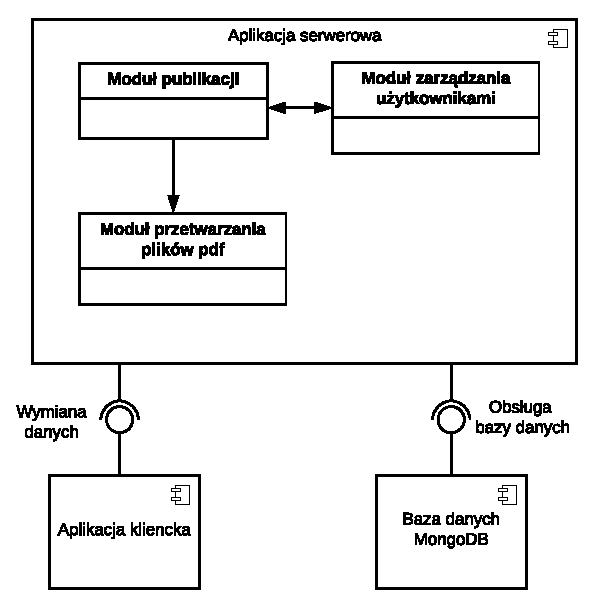
\includegraphics[scale=1.2]{\ImgPath/rys/diag_komp_ogolny.pdf}
 	\end{center}
 	\caption{Ogólna architektura systemu.}
 	\label{ogolnaArchitektura}
 \end{figure}
 Przedstawiona na powyższym diagramie aplikacja serwerowa oraz baza danych MongoDB będę uruchamiana jako kontenery Dockera, natomiast aplikacja kliencka będzie pracowała na urządzeniach z systemem Android. Wymiana danych pomiędzy tymi aplikacjami będzie odbywała się za pomocą interfejsu programistycznego(API), w sposób szyfrowany przy wykorzystaniu protokółu HTTPS.
 Baza danych będzie działać w wewnętrznej sieci Dockerowej, do której bezpośredni dostęp będzie posiadała jedynie aplikacja serwerowa. 

\section{Architektura aplikacji serwerowej}
\subsection{Struktura}
Aplikacja serwerowa zbudowana będzie w oparciu o środowisko Node.js. Składać się będzie z 3 podstawowe modułów:
\begin{enumerate}
	\item Moduł zarządzania użytkownikami -- będzie odpowiadał za obsługę żądań HTTP dotyczących rejestracji i logowania użytkowników oraz zarządzaniu sesją
	
	\item Moduł publikacji -- będzie posiadał następujące zadania:
	\begin{itemize}
		\item obsługa żądań HTTP dotyczących publikacji;
		\item zapis, odczyt i modyfikacja publikacji w bazie danych;
		\item zlecanie operacji przetwarzania pliku PDF;
		\item zapisywanie i odczyt plików PDF przypisanych do publikacji.
	\end{itemize}
	 
	\item Moduł przetwarzania plików pdf -- jako jedyny nie będzie odpowiadał za obsługę żądań, a za przetwarzania plików PDF. Do przetwarzania plików pdf zostanie wykorzystana biblioteka \textit{pdf--parse}. Będzie dostarczał następujące funkcjonalności:
	\begin{itemize}
		\item odczyt informacji takich jak tytuł lub autor publikacji z metadanych plików PDF;
		\item wyszukiwanie DOI w metadanych pliku PDF, bądź w jego treści;
		\item pobieranie szczegółów dotyczących przetwarzanej publikacji na podstawie znalezionego wcześniej numery DOI.
	\end{itemize}
\end{enumerate}


Dodatkowo żądania HTTP będą przetwarzane wstępnie, także przez następujące moduły pośredniczące:
\begin{enumerate}
	\item Moduł autoryzacyjny -- jego rolą będzie sprawdzanie czy dane żądanie wysłane zostało przez użytkownika, który posiada uprawnienia do jego wykonania
	\item Moduł walidacji danych -- będzie odpowiedzialny za sprawdzania czy dane przychodzące w żądaniach, typu POST oraz PUT, które tworzą lub modyfikują informacje w bazie danych, są w odpowiednim formacie
\end{enumerate}


\subsection{Środowisko}
Aplikacja serwerowa będzie przygotowana do pracy jako kontener Dockera. Dzięki temu przy wdrażaniu aplikacji konfiguracja środowiska produkcyjnego, nie będzie wymagała pełnego przygotowania środowiska Node.js, potrzebując do pracy jednie aplikacji Docker oraz docker--compose, która pozwala na zarządzanie i konfigurację wielu kontenerów, mogących współpracować między sobą. Dzięki temu, że baza danych MongoDB może również działać w formie kontenera Dockerowego, przy wykorzystaniu aplikacji docker--compose, uruchomienie całej aplikacji serwerowej wraz bazą danych będzie ograniczać się do pobrania kontenerów oraz ich uruchomienia za pomocą jednego polecenia, a dodatkowo pozwala na wdrożenie aplikacji zarówno przy użyciu systemu Linux i Windows jaki i macOS.

\section{Architektura aplikacji klienckiej}
Aplikacja kliencka będzie przeznaczona na urządzenia mobilne z systemem Android. Zostanie wykonana w sposób natywny dla tej platformy przy wykorzystaniu środowiska Android Studio oraz języka Kotlin. Zgodnie z zaleceniami występującymi w dokumentacji Android, wykorzystany zostanie uproszczony wzorzec Model–View–Viewmodel(MVVM). 

\subsection{Wzorzec Model–View–Viewmodel(MVVM)}
Wzorzec MVVM bazuje na popularnym wzorcu Model--View--Controller. Jest często wykorzystywany podczas tworzenia aplikacji z interfejsem graficznym, do których możemy zaliczyć programy przeznaczone na system Android. 
Zgodnie z tą architekturą aplikacja składa się z głównych elementów:
\begin{enumerate}
	\item model -- przechowuje dane, pobrane przez viewmodel, później prezentowane w warstwie view, nie powinien zawierać logiki biznesowej,
	\item view -- jest to reprezentacja graficznego widoku, widzianego przez użytkownika aplikacji,
	\item viewmodel -- element spajający model i view, pod pewnym względem odpowiadający dla wartswy controller z wzorca MVC. Jest odpowiedzialny za wypełnianie widoku danymi, pobranymi z modelu oraz za obsługę interakcji w użytkownikiem. 
\end{enumerate}

Jedną z podstawowych cech tego wzorca jest tak zwane wiązanie danych. Polega ono na automatycznym odświeżaniu danych pochodzących z modelu w widoku, w momencie gdy dojdzie do ich modyfikacji w viewmodelu. Dzięki temu, programista jest zwolniony z ciągłego dbania o uaktualnianie danych prezentowanych w widoku.

\newpage
\subsection{Struktura}
Natywne aplikacje działające pod kontrolą systemu Android zbudowaną są z komponentów zwanych aktywnościami (Activity). Zgodnie z definicją dostępną w dokumentacji\footnote{\url{https://developer.android.com/reference/android/app/Activity}}, jest to  pojedyncza konkretna czynność, która może zostać wykonana przez użytkownika. Dodatkowo aktywności mogą składać się z mniejszych części zwanych fragmentami. Aplikacja kliencka przygotowywana w ramach tej pracy, będzie składała się z trzech aktywności:
\begin{enumerate}
	\item LoginActivity -- aktywność odpowiedzialna za proces logowania użytkownika.
	
	\item MainActivity -- główna aktywność służąca do prezentacji listy publikacji danego użytkownika. 

	\item PublicationDetailsActivity -- aktywność w której dodaje się nowe publikacje oraz odczytuje i edytuje istniejące.

\end{enumerate}

Do komunikacji z aplikacja serwerową za pomocą protokołu HTTP wykorzystana zostanie biblioteka Retrofit. Wykorzystywana będzie w klasach należących do paczki \textit{network}, która odpowiadać za obsługę żądań HTTP wykorzystywanych do logowania użytkowników oraz do odczytywania, dodawania i edycji publikacji naukowych. 

Do obsługi asynchroniczności zapytań, wszystkie klasy korzystające z klas pakietu \textit{network}, będą wymagały zaimplementowania interfejsu \textit{RequestObserver}, który będzie zawierał dwie metody:
\begin{enumerate}
	\item onSuccess -- metoda wywoływana, w przypadku gdy żądanie zakończyło się pomyślnie.
	
	\item onFail -- metoda wywoływana, w przypadku gdy żądanie zakończyło się błędem.
\end{enumerate}
\chapter{Szczegóły implementacyjne aplikacji serwerowej}
\section{Ogólna struktura}
Zgodnie z przedstawioną w poprzednim rozdziale architekturą aplikacji serwerowej została ona podzielona na trzy moduły. W tym rozdziale zostaną przedstawione ich szczegóły implementacyjne oraz sposób komunikacji pomiędzy sobą. Organizacja kodu aplikacji serwerowej została przedstawiona, na poniższym Rysunku 4.1.

 \begin{figure}[!htbp]
	\begin{center}
		\centering
		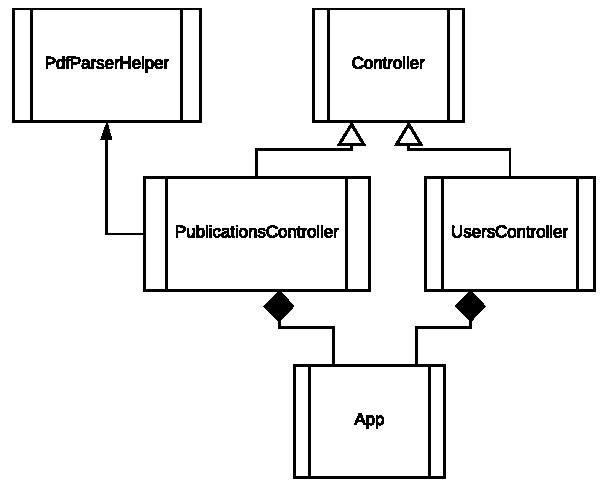
\includegraphics[scale=0.91]{\ImgPath/rys/diag_klas_serwer.pdf}
	\end{center}
	\caption{Diagram klas.}
	\label{diagramKlas}
\end{figure}
\subsection{Opis podstawowych klas}
Przedstawione na powyższym diagramie klasy pełnią następujące funkcje:
\begin{enumerate}
	\item App -- główna klasa aplikacji, która inicjalizuje wszystkie klasy rozszerzające klasę Controller, a także odpowiedzialna za skonfigurowanie oprogramowania pośredniczącego (middleware)\cite{Middleware};
	
	\item Controller -- klasa rozszerzana przez inne klasy, odpowiedzialne za obsługę żądań  HTTP;
	
	\item UsersController -- klasa obsługująca żądania dotyczące rejestracji, logowania, oraz wylogowywania użytkowników;
	
	\item PublicationsController -- klasa obsługująca żądania dotyczące dodawania, odczytywania, usuwania oraz edycji publikacji.
	
\end{enumerate}

\section{Obsługa użytkowników}
Cała obsługa użytkowników w systemie została napisana od podstaw. Odpowiedzialna jest za to klasa \textit{UsersController}, odpowiadająca za proces rejestracji i logowania użytkowników oraz oprogramowanie pośredniczące \textit{authMiddleware}, którego zadaniem jest sprawdzanie czy dane żądanie jest wykonywane przez zalogowanego użytkownika, który posiada wystarczające uprawnienia. Do zapewnienia bezpiecznego przechowywania hasła wykorzystana została biblioteka \textit{bcrypt}, za pomocą której uzyskiwana jest sól, wykorzystywana podczas obliczania funkcji skrótu dla hasła. 

Dla celów autoryzacji, dokumenty reprezentujące użytkowników, które przechowywane są w bazie danych, posiadają w swojej strukturze dwa pola:
\begin{itemize}
	\item email -- służący do identyfikacji, użytkownika, który próbuje zalogować się do systemu;
	
	\item hash -- pole zawierające sól oraz wynik funkcji skrótu dla hasła danego użytkownika;
	
	\item type -- pole służące do określania typu użytkownika. Obecnie nie jest one wykorzystywane i zawsze posiada wartość \textit{USER}, lecz umożliwia wprowadzenie w przyszłości podziału użytkowników na różne grupy, o specyficznych uprawnieniach.
	
\end{itemize}
Dzięki przechowywaniu wyniku funkcji skrótu dla hasła, zamiast jawnego jego przechowywania, podnoszony jest poziom bezpieczeństwa. Nawet w przypadku, gdy dane z bazy danych zostaną wykradzione, hasła użytkowników systemu nie będą mogły zostać odczytane. Wynika to z własności funkcji skrótu, która nie pozwala w łatwy sposób odczytać wartości wejściowej, nawet przy posiadania soli, która została wykorzystana podczas obliczania wyniku funkcji.


\subsection{Proces rejestracji użytkownika}
Proces rejestracji użytkownika został przedstawiony na Rysunku 4.2:
 \begin{figure}[!htbp]
	\begin{center}
		\centering
		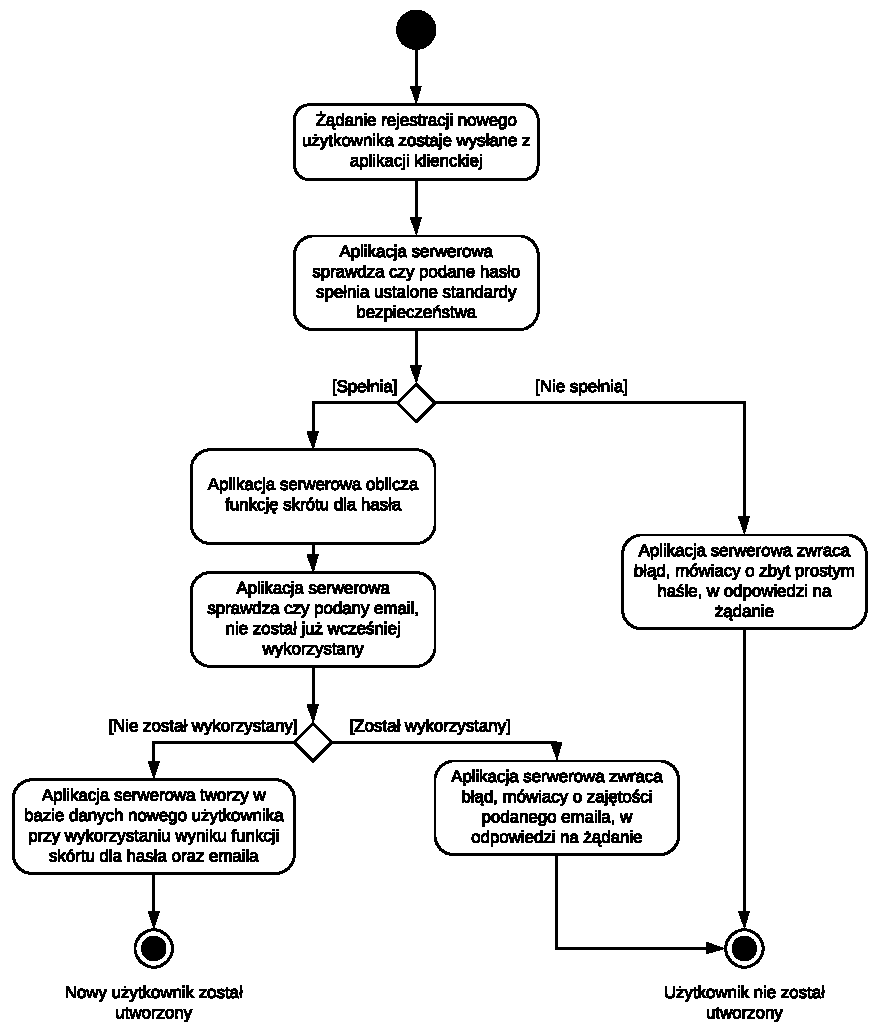
\includegraphics[scale=0.8]{\ImgPath/rys/diag_aktyw_rejestr.pdf}
	\end{center}
	\caption{Diagram aktywności dla procesu rejestracji.}
	\label{diagramAktywnosciRejstracja}
\end{figure}
\newpage

\subsection{Proces logowania użytkownika}
Po pomyślnym przejściu procesu rejestracji, użytkownik nabywa możliwość zalogowania się do systemu za pomocą wcześniej podanego emaila i hasła. Proces ten został zaprezentowany na Rysunku 4.3.


\begin{figure}[!htbp]
	\begin{center}
		\centering
		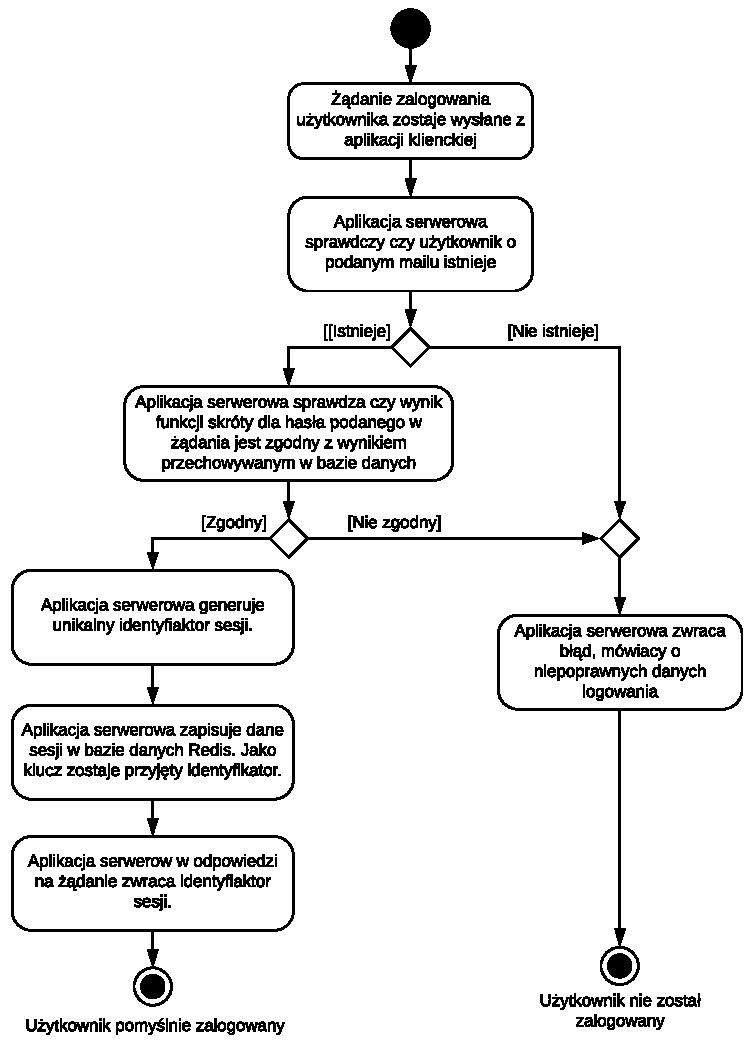
\includegraphics[scale=0.92]{\ImgPath/rys/diag_aktyw_logowanie.pdf}
	\end{center}
	\caption{Diagram aktywności dla procesu logowania.}
	\label{diagramAktywnosciLogowanie}
\end{figure}
\newpage
W celu przeprowadzania logowania do systemu, wysyłane jest żądanie do aplikacji serwerowej z danymi, na podstawie, których użytkownik jest uwierzytelniany, a w odpowiedzi zwracany jest identyfikator sesji, który jest później wykorzystywany podczas wysyłania innych żądań. Posiada on ograniczoną czasową ważność, wynoszącą 7 dni.



\section{Uwierzytelnienie i autoryzacja żądań}
Większość żądań obsługiwanych przez aplikacją serwerową, może być obsłużona tylko w przypadku, gdy użytkownik, które je wysłał został poprawnie uwierzytelniony i zautoryzowany. 
Autoryzacja żądania odbywa się na podstawie weryfikacji nagłówka żądania HTTP o nazwie \textit{Authorization}, który powinien zawierać żeton pełniący rolę identyfikatora sesji. Za to zadanie odpowiedzialne są dwie funkcje pośredniczące w obsłudze żądania: 
\begin{enumerate}
	
	\item \textit{authMiddlewareUser} -- funkcja zezwala na pełne wykonanie żądania, tylko gdy użytkownik jest zalogowany.
	
	\item \textit{authMiddlewareOwner} -- funkcja zezwala na pełne wykonanie żądania, tylko gdy użytkownik jest właścicielem zasobu, którego dotyczy żądanie.
	
\end{enumerate}

Obie te funkcje wykorzystują w trakcie działania jedną z najważniejszych funkcji biorących udział w procesie obsługi użytkowników o nazwie \textit{checkAuth}. Jej rolą jest sprawdzenie ważności sesji i zgodności roli użytkownika zidentyfikowanego na podstawie żetonu przesłanego w nagłówkach żądania, z wymaganiami bezpieczeństwa danego żądanie. Jeśli warunki te są spełnione, wtedy obsługa żądania przekazywana jest już do docelowej funkcji. 

Nagłówek funkcji \textit{checkAuth} został zaprezentowany na Listingu 4.1.

\begin{lstlisting}[caption=Sygnatura funkcji checkAuth,label=code1,captionpos=b]
async function checkAuth: boolean (
	req: Request,
	next: NextFunction,                        
	profileTypes: string[]
)
\end{lstlisting}



Do wywołania tej funkcji należy jej przekazać następujące parametry:
\begin{enumerate}
	
	\item req -- obiekt zawierający wszystkie parametry żądania, takie jak nagłówki czy ciało,
	
	\item next -- funkcja, która powinna zostać wywołana jako kolejna, podczas procesu obsługi żądania, w przypadku gdy obecnie wykonywana funkcja zakończy się prawidłowo,
	
	\item profileTypes -- tablica zawierająca role użytkowników, którzy mają prawo do wywołania danego żądania.
\end{enumerate}

\subsection{Sposób działania funkcji checkAuth}
Na początku działania, sprawdza czy w żądaniu, które zostało odebrane, znajduje się nagłówek \textit{Authorization} zawierający żeton identyfikujący sesję użytkownika. Jeśli żeton został odnaleziony, na jego podstawie wyszukiwany jest obiekt sesji w bazie danych Redis. Jeśli wyszukiwanie powiedzie się, funkcja \textit{checkAuth} przeprowadza następujące czynności:
\begin{enumerate}	
	\item Sprawdzenie czy czas ważności sesji nie został przekroczony, poprzez odczytanie czasu ważności z obiektu sesji, na następnie porównanie go z czasem obecnym. 
	
	\item Sprawdzenie czy rola użytkownika, którego sesja została zidentyfikowana, jest zgodna z parametrem \textit{profileTypes}. Zgodność określana jest na poprzez sprawdzenie czy typ użytkownika odczytany z obiektu sesji znajduje się w tablicy \textit{profileTypes}.
\end{enumerate}
W przypadku nie odnalezienia nagłówka \textit{Authorization} lub obiektu sesji w bazie danych Redis, funkcja zwraca wartość \verb|false|, która oznacza, że proces autoryzacji również zostanie zakończony niepomyślnie. W przypadku gdy wszystkie wyżej wymienione warunki zostaną spełnione, do obiektu żądania zostaną dopisane parametry użytkownika powiązanego z sesją a następnie funkcja zwróci wartość true, która oznacza, że proces autoryzacji użytkownika zakończył się pomyślnie.

\subsection{Funkcja authMiddlewareUser}
Funkcja authMiddlewareUser wykorzystuje wzorzec projektowy Adapter, w celu dostosowania funkcji \textit{checkAuth} do interfejsu, funkcji pośredniczących w środowisku Node.js. Jej sygnatura została przedstawiona na Listingu 4.2.
\begin{lstlisting}[caption=Sygnatura funkcji authMiddlewareUser,label=code1,captionpos=b]
async function authMiddlewareUser: void (
	req: Request,
	res: Response,
	next: NextFunction
)
\end{lstlisting}
W odróżnieniu od funkcji \textit{checkAuth} wśród argumentów wejściowych brakuje parametru \textit{profileTypes}, będącego listą ról użytkowników, którzy mają prawo do wywołania danego żądania. Dodatkowo w celu zapewnienia zgodności z interfejsem funkcji pośredniczącej w Node.js, pojawił się parametr \textit{res}, który jest obiektem odpowiedzi na żądanie.   

Jej działanie polega na wywołaniu funkcji \textit{checkAuth} oraz sprawdzeniu czy zwróci ona wartość \verb|true|. Jeśli tak się stanie, wywoływana jest funkcja \textit{next}, która jest następną funkcją odpowiedzialną za przetworzenie żądania.
Przy wywoływaniu funkcji \textit{checkAuth}, jako parametr \textit{profileTypes}  zawsze zostaje przekazana tablica \verb|[ "USER" ]|, co oznacza, że obługa żądania będzie kontynuowana, tylko gdy użytkownik, z którym będzie powiązany identyfikator sesji zawarty w nagłówku żądania jest typu \verb|USER|. 

Ze względu na to, że obecnie wszyscy użytkownicy posiadają typ \verb|USER|, funkcja \textit{authMiddlewareUser} pozwala w rzeczywistości na badanie czy użytkownik wywołujący żądanie jest zalogowany.

\subsection{Funkcja authMiddlewareOwner}
Funkcja \textit{authMiddlewareOwner} w odróżnieniu \textit{authMiddlewareUser}, nie posiada interfejsu zgodnego z funkcjami pośredniczącymi, gdyż wykorzystuje ona domknięcie, zwracając funkcję, posiadającą interfejs funkcji pośredniczącej.


Jedynym argumentem, który przyjmuje funkcja \textit{authMiddlewareOwner} jest obiekt \textit{DBModel} typu \textit{Model<IOwnership  Document>} pochodzącego z biblioteki Mongoose, który służy do zarządzania wybranym rodzajem dokumentów w bazie danych MongoDB. Do funkcji może zostać przekazany jedynie taki model, który obsługuje dokumenty które są jednocześnie implementują interfejs \textit{Document}, który również pochodzi  z biblioteki Mongoose i reprezentuje pojedynczy dokument z bazy danych oraz \textit{IOwnership}, który wykorzystywany jest we wszystkich dokumentach, które mogą posiadać właścicieli, jak ma to miejsce przykładowo dla dokumentów przechowujących dane pojedynczej publikacji. 

Interfejs \textit{IOwnership} został przedstawiony na Listingu 4.3.
\begin{lstlisting}[caption=Interfejs IOwnership,label=code1,captionpos=b]
interface IOwnership {
	owners: UserType[]
} 
\end{lstlisting}
Interfejs ten jest bardzo prosty i posiada tylko jedno pole \textit{owners}, które jest tablicą użytkowników, będących właścicielami obiektu, który implementuje ten interfejs. Dzięki zastosowaniu tego interfejsu, nie ma potrzeba pisania osobnej obsługi rozpoznawania czy użytkownik jest właścicielem wybranego obiektu, dla każdego rodzaju dokumentów osobno. Z tej właśnie własności korzysta funkcja \textit{authMiddlewareOwner}.

Uproszczony kod funkcji \textit{authMiddlewareOwner} został przedstawiony na Listingu 4.4.
\begin{lstlisting}[caption=Sygnatura funkcji authMiddlewareOwner,label=code1,captionpos=b]
const authMiddlewareOwner = (DbModel: Model<IOwnership & Document>) => (
  async (req: Request, res: Response, next: NextFunction) => {
	const authStatus = await checkAuth(req, next, [USER, ADMIN]);
	if (authStatus) {	
		const { documentId } = req.params;
		const { _id as userId } = (<any>req).user;
		let user: UserType = await User.findById(userId);
		dbObject = await DbModel
			.findOne({ _id: documentId, owners: user });
	}           
  }
)
\end{lstlisting}

Jej działanie opiera się o domknięcie -- jako argument otrzymuje ona obiekt modelu, który później zostaje zawarty w środowisku zwracanej funkcji. Dzięki temu, że model ten musi implementować interfejs \textit{IOwnership}, dokumenty, które zostaną pobrane z bazy danych za jego pomocą muszą posiadać pole \textit{owners}, określające ich właścicieli.
Zatem funkcja  \textit{authMiddlewareOwner} po wywołaniu zwraca inną funkcję, która jest już właściwą funkcją pośredniczącą, zawierającą dodatkowo w swoim środowisku odwołanie do obiektu modelu dokumentu z bazy danych. 

Wywołanie funkcji \verb|authMiddlewareOwner(Publication)|, zwróci funkcję pośredniczą, która pozwoli na wywołanie kolejnej metody obsługującej żądanie, tylko gdy użytkownik wywołujący żądanie, jest właścicielem obiektu typu \verb|Publication|, którego id została przekazane jako parametr w ścieżce żądania.

\begin{enumerate}
	
	\item W sposób analogiczny do funkcji \textit{authMiddlewareUser}, wykorzystując funkcję \textit{checkAuth}, sprawdzana jest tożsamość i typ użytkownika, który wysłał żądanie.
	
	\item Jeśli funkcja \textit{checkAuth} potwierdzi, to że użytkownik jest zalogowany oraz to czy jego typ jest odpowiedni, sprawdzane jest czy dokument, którego dotyczy żądanie jest własnością tego użytkownika. 
	
	\item Jeśli użytkownik okaże się właścicielem dokumentu, wywoływana jest funkcja \textit{next}, która jest następną funkcją odpowiedzialną za przetworzenie żądania.
\end{enumerate}

Dzięki tej funkcji, nie trzeba każdorazowo sprawdzać czy użytkownik wysyłający żądanie usunięcia lub edycji danego dokumentu, ma do tego prawo, co ułatwia bezpośrednio kod tych funkcji które wykonują już właściwe operacje na dokumentach przechowywanych w bazie danych.

\subsection{Proces wylogowania użytkownika}
Proces wylogowywania użytkownika jest stosunkowo prosty i polega najpierw na jego zidentyfikowaniu przy pomocy funkcji pośredniczącej \textit{authMiddlewareUser}, a następnie na usunięciu danych dotyczących jego sesji z bazy danych Redis. Dzięki temu, pomimo że identyfikator sesji może pozostać zapisany po stronie klienta, wysłane żądanie zawierające ten identyfikator nie zostanie wykonane.
\newpage
\section{Zarządzanie publikacjami oraz przetwarzanie plików pdf}
W bazie danych MongoDB dokument reprezentujący publikację posiada następujące pola: 
\begin{enumerate}
	
	\item \verb|name: string| -- tytuł publikacji. Może zostać odczytany podczas  z pliku PDF.
	
	\item \verb|authors: string[ ]| -- tablica zawierająca autorów publikacji. Pole to nie powinno być mylone z \verb|owners: UserType[ ]|, który w odróżnieniu od \verb|authors: string[ ]|, przechowuje właścicieli publikacji
	
	\item \verb|file: string| -- ścieżka do pliku PDF 
	
	\item \verb|description: string| -- opis publikacji
	
	\item \verb|doi: string| -- nr doi publikacji
\end{enumerate}
Dodatkowo zawiera pole \textit{owners} pochodzące z interfejsu \textit{IOwnership}, co pozwala korzystać z funkcji pośredniczącej \textit{authMiddlewareOwner}, w odniesieniu do publikacji.

Zarządzanie publikacjami odbywa się poprzez obsługę 7 żądań. Aby wywołać każde z nich użytkownik wcześniej zalogować się do systemu. Posiadają one następujące funkcjonalnościach:
\begin{enumerate}
	
	\item Żądanie typu GET -- pobranie informacji dotyczących pojedynczej publikacji. Aby pobrać publikację 
	
	\item Żądanie typu GET -- pobranie listy z informacjami o wszystkich publikacjach użytkownika. 
		
	\item Żądanie typu PUT -- edycja informacji dotyczących pojedynczej publikacji.
	
	\item Żądanie typu DELETE -- Usunięcie informacji i pliku pdf należących do pojedynczej publikacji.
	
	\item Żądanie typu GET -- pobranie pliku pdf przypisanego do wybranej publikacji.
	
	\item Żądanie typu POST -- przetworzenie pliku pdf. Jako odpowiedź zwracane było informacje, które udało się odczytać z wysłanego pliku pdf.
	
	\item Żądanie typu POST -- dodanie nowej publikacji.
\end{enumerate}
\pagebreak
Pierwsze pięć wymienionych wyżej opiera się o zwykłe operacje CRUD przeprowadzane na bazie danych, natomiast dwa pozostałe zależne od siebie żądania również korzystają z bazy danych, lecz wykonują także inne czynności, takie jak operacje na plikach, czy też komunikacja z API służącym do pobierania informacji na temat danej publikacji na podstawie wyszukanego wcześniej numeru DOI.


\subsection{Definiowanie żądań}

Przykładowa deklaracja obsługi żądania została przedstawiona na Listingu 4.5.

\begin{lstlisting}[caption=Deklaracja obsługi żądania,label=code1,captionpos=b]
router.get(
	'/:id', 
	authMiddlewareOwner(Publication), 
	getPublication
)
\end{lstlisting}
Przedstawiony w powyższym fragmencie obiekt \verb|router|, służy do definiowania sposobu obsługi żądań. W celu dodania nowego żądania, należy wywołać metodę on nazwie zgodnej z jego typem. Przykładowo w celu dodania obsługi żądania GET należy wywołać metodę \verb|get|. Każda z tych metod jako pierwszy argument przyjmuje ścieżkę żądania, a następnie funkcje obsługujące żądnie, gdzie pozycja wśród argumentów odpowiada kolejności, w której poszczególne funkcje będą wywoływane. Zatem w przypadku dla powyższej próbki kodu po odebraniu żądania, najpierw wywołana zostanie metoda zwrócona przez funkcję \verb|authMiddlewareOwner(Publication)|, a następnie w zależności wyniku działania tej funkcji może zostać wywołana funkcja \verb|getPublication| lub też obsługa żądania może zakończyć się błędem przed wywołaniem tej funkcji.


\subsection{Pobranie listy publikacji}
Proces ten polega na wyszukaniu w bazie danych tych dokumentów opisujących publikacje, których właścicielem jest użytkownik rozpoznany podczas procesu autoryzacji.
\pagebreak

Uproszczony kod funkcji został przedstawiony na Listingu 4.6.
\begin{lstlisting}[caption=Funkcja getPublication,label=code1,captionpos=b]
const getPublication = () => {
	const { _id as userId } = (<any>req).user;
	user = await User.findById(userId);
	const publications = await Publication.find({owners: user});
}
\end{lstlisting}
\subsection{Pobranie dokumentu pojedynczej publikacji}
Proces rozpoczyna się od sprawdzenia czy użytkownik wywołujący to żądanie, jest właścicielem publikacji, której szczegóły próbuje odczytać. Jeśli tak jest, publikacja zostaje wyszukana w bazie danych i zwrócona użytkownikowi.

\subsection{Edycja dokumentu pojedynczej publikacji}
Początek obsługi tego żądania jest taki sam jak w przypadku pobrania pojedynczej publikacji -- najpierw sprawdzane jest użytkownik wywołujący to żądanie, jest właścicielem publikacji, którą próbuje edytować. Jeśli tak publikacja zostaje zedytowana zgodnie z danymi otrzymanymi w żądaniu.

\subsection{Usunięcie pojedynczej publikacji}
Analogicznie to dwóch wyżej wymienionych żądań, w przypadku usuwania aplikacji, najpierw sprawdzane jest użytkownik wywołujący to żądanie, jest właścicielem publikacji, a następnie dochodzi do usunięcia dokumentu zawierającego jej szczegółu oraz PDF do niej należącego.

\subsection{Pobranie pliku PDF nalezącego do pojedynczej publikacji}
Obsługa tego żądania jest niemal identyczna do obsługi pobierania dokumentu pojedynczej publikacji, z tą różnicą, że zamiast zwracać obiekt, zwracany jest plik, którego ścieżka zapisana jest w dokumencie wybranej publikacji.

\subsection{Przetwarzanie plików PDF}
Funkcja przetwarzająca plik PDF jest wywoływana podczas obsługi żądania przetwarzania pliku PDF. Proces ten polega na przeszukaniu treści pliku oraz jego metadanych w celu odnalezienia identyfikatora DOI, który zostanie wykorzystany później w celu pobrania szczegółów dotyczących publikacji. Jeśli identyfikator DOI nie zostanie odnaleziony, następuje wtedy próba odczytania informacji o publikacji wprost z metadanych pliku PDF.

W przypadku, gdy identyfikator DOI nie zostanie odnaleziony wśród metadanych pliku, jego poszukiwanie w treści pliku wykonywane jest przy użyciu wyrażenia regularnego, co przedstawione zostało Listingu 4.7.

\begin{lstlisting}[caption=Wykorzystanie wyrażenia regularnego do poszukiwania DOI,label=code1,captionpos=b]
const regex = /\S+(doi.org)\S+/g;
const found = pdfData.text.match(regex);
}
\end{lstlisting}
Stała \verb|regex| zawiera w sobie definicję poszukiwanego ciągu znaków. Obiekt pdfData powstaje w wyniku wykorzystania funkcji dostarczonej w bibliotece \textit{pdf--parse}. Polę text należące do tego obiektu, zawiera cały tekst znajdujący się wewnątrz przetwarzanego pliku. Przy wykorzystaniu funkcji \verb|match|, która wyszukuje ciągi tekstu zgodne z wyrażeniem regularnym, który został przekazany do funkcji jako argument, wyszukiwane są wszystkie możliwie identyfikatory DOI zawarte w pliku. Jako właściwy identyfikator DOI zostaje uznany ten, który jako pierwszy zostanie odnaleziony w tekście, gdyż z duża dozą prawdopodobieństwa pozostałe identyfikatory należą do innych publikacji, do których występują odwołania, wewnątrz badanego pliku.

Jeśli identyfikator DOI został pomyślnie odnaleziony, następuje próba pobrania na jego podstawie szczegółów dotyczących publikacji. Następnie pobrane dane są uzupełniane o te odczytane bezpośrednio z metadanych pliku PDF.

Gdyby identyfikator DOI nie został odnaleziony, nastąpiła by próba odczytania wszystkich wartości wprost z metadanych pliku. Jeśli i ta operacja zakończyła by się niepowodzeniem, użytkownik będzie musiał ręcznie wprowadzić wszelkie szczegóły dotyczące publikacji.

\subsection{Dodawanie publikacji na podstawie pliku PDF}
Proces dodawania publikacji, składa się dwóch podstawowych kroków:
\begin{enumerate}
	\item Przetworzenie pliku pdf, w wyniku którego mogą zostać odczytane informacje dotyczące publikacji.
	\item Zapisanie publikacji, po zreadgowaniu i uzupełnieniu przez użytkownika informacji na temat publikacji, które pochodzą z procesu przetwarzania
\end{enumerate}
Cały proces składa się także z dwóch osobnych żądań: 
\begin{enumerate}	
	\item Żądanie przetwarzające plik PDF -- w ramach ciała żądania wysyłany jest plik PDF, który zostaje zapisany w lokalizacji tymczasowej, a w odpowiedzi zwracane są informacje, które udało się odczytać z pliku.  Proces obsługi żądania prezentuje Rysunek 4.4:
	\begin{figure}[!htbp]
		\begin{center}
			\centering
			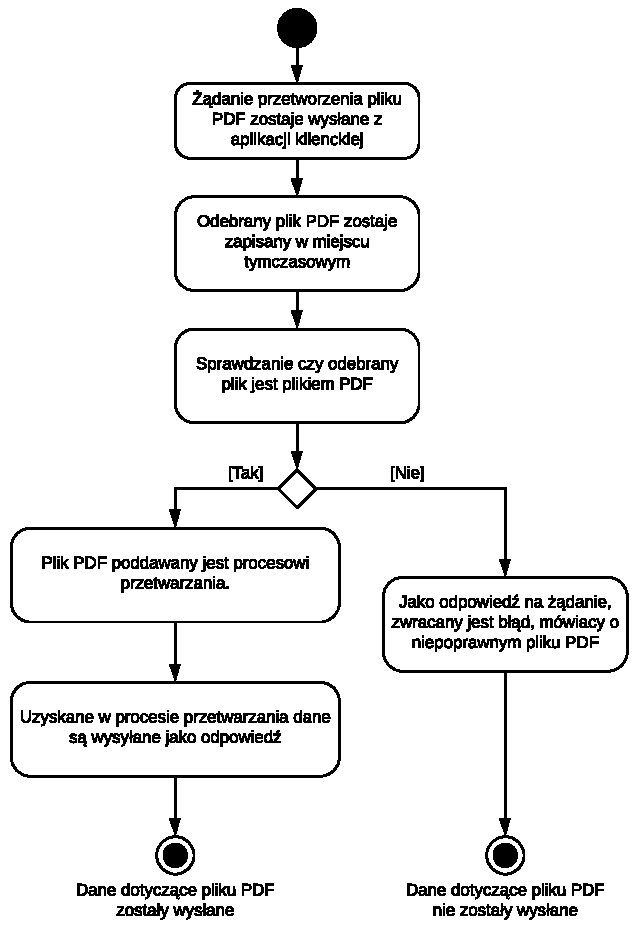
\includegraphics[scale=0.873]{\ImgPath/rys/diag_aktyw_wstepne_przetwarzanie.pdf}
		\end{center}
		\caption{Diagram aktywności dla obsługi żądania przetwarzania pliku PDF.}
		\label{diagramAktywnosciDodawanie}
	\end{figure}
	
	\item Żądanie dodające dokument publikacji -- w ciele żądania powinny znajdować się informacje pochodzące z wcześniejszego przetwarzania pliku PDF, które zostały zredagowane przez użytkownika. Wśród odebranych parametrów publikacji, musi znaleźć się identyfikator przetworzonego wcześniej pliku PDF. Proces obsługi żądania został zaprezentowany na Rysunku 4.5:
	\begin{figure}[!htbp]
		\begin{center}
			\centering
			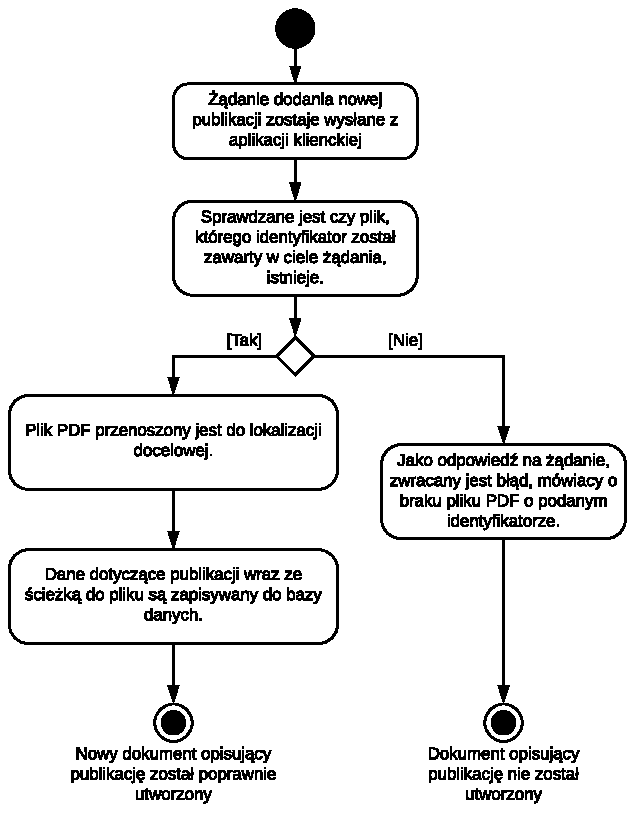
\includegraphics[scale=1]{\ImgPath/rys/diag_aktyw_dodawanie_pub.pdf}
		\end{center}
		\caption{Diagram aktywności dla procesu dodawania publikacji.}
		\label{diagramAktywnosciDodawanie}
	\end{figure}
	
\end{enumerate}


\section{Walidacja danych}
W celu zwiększenia bezpieczeństwa oraz łatwiejszego odnajdowania błędów użytkownika, ciała prawie wszystkich żądań typu POST i PUT, są walidowane, po procesie autoryzacji użytkownika ale przed wywołaniem właściwej funkcji obsługującej żądanie. Do tego celu wykorzystana została funkcja pośrednicząca \textit{validationMiddleware}. 

W swoim działania funkcja ta korzysta z biblioteki \textit{class--validator}, która umożliwia walidowanie obiektów wykorzystując zdefiniowane wcześniej do tego celu wzorce. Wykorzystuje ona również domknięcie, zwracając funkcję, która jest zgodna z interfejsem funkcji pośredniczącej.

Sygnatura funkcji \textit{validationMiddleware} została zaprezentowana na Listingu 4.8. 

\begin{lstlisting}[caption=Sygnatura funkcji validationMiddleware,label=code1,captionpos=b]
function validationMiddleware<T>(type: any): RequestHandler
\end{lstlisting}
Jej jedynym argumentem jest obiekt, będący definicją typu, z którym musi być zgodne ciało żądania, do którego obsługi wykorzystana została ta funkcja.

Przykładowa definicja typu, który musi być zgodny z ciałem żądania dodającego publikację przedstawiona została na Listingu 4.9.
\begin{lstlisting}[caption=Klasa AddPublicationDto,label=code1,captionpos=b]
class AddPublicationDto {
	@IsString()
	public readonly name: string;
	
	@IsString()
	public readonly description: string;
	
	@IsString()
	public readonly file: string;
	
	@IsArray()
	@ValidateNested({ each: true })
	@ArrayMinSize(0)
	@Type(() => String)        
	public readonly authors: string[];
}
\end{lstlisting} 
\pagebreak

Definiowanie warunków, które muszą zostać spełnione przez poszczególne pola ciała żądania definiowane są za pomocą dekoratorów. Znaczenie części z tych, które zostały wykorzystane w powyższym przykładzie jest następujące: 
\begin{itemize}
	\item \verb|@IsString()| -- sprawdza czy wartość danego pola jest ciągiem znaków;
	\item \verb|@IsArray()| -- sprawdza czy wartość danego pola jest tablicą; 
	\item \verb|@ValidateNested()| -- określa czy w przypadku tablic oraz obiektów należy walidować, każdą zagnieżdżoną wartość ;
	\item \verb|@ArrayMinSize(0)| -- służy do określenia minimalnej wielkości tablicy.
\end{itemize}

\chapter{Szczegóły implementacyjne aplikacji klienckiej}

Aplikacja kliencka przygotowana w ramach tego projektu, została napisana w celu działania na urządzeniach mobilnych wyposażonych w system Android. Zgodnie z informacjami zawartymi w poprzednich rozdziałach, będzie ona wykorzystywać wzorzec Model--View--Viewmodel(MVVM) oraz do jej stworzenia wykorzystany został język Kotlin. 

Najważniejsze klasy definiujące trzy aktywności, z których składa się aplikacja kliencka należą do podstawowego pakietu publicationManager.
Dodatkowo aplikacja została podzielona następujące podpakiety:
\begin{enumerate}
 	\item network -- zawiera wszystkie klasy odpowiedzialne za wymianę danych z aplikacją serwerową, przy użyciu żądań wysyłanych za pomocą protokołu HTTP
 	\item ui -- składa się z klas odpowiedzialnych za obsługę interfejsu użytkownika.
 	\item interfaces -- w tym pakiecie znajdują się interfejsy wykorzystywane wewnątrz aplikacji, służące między innymi do obsługi odpowiedzi na żądania
 	\item utils -- w skład tego pakietu wchodzą różnego rodzaju klasy i funkcje pomocnicze
\end{enumerate}

Oprócz kodu napisanego w języku Kotlin, aplikacja składa się także z plików XML. Są one wykorzystywane do konfiguracji ustawień wymaganych przez system Android, a także do definiowania styli oraz układu poszczególnych elementów interfejsu użytkownika. 

\section{LoginActivity}
LoginActivity jest pierwszą aktywnością, która jest uruchamiana po włączeniu aplikacji. Zgodnie z nazwą, odpowiada ona za obsłużenie procesu logowania użytkownika, a także za sprawdzenie czy użytkownik nie zalogował się wcześniej do aplikacji. Jej sposób działania zaprezentowany został na Rysunku 5.1.
\begin{figure}[!htbp]
	\begin{center}
		\centering
		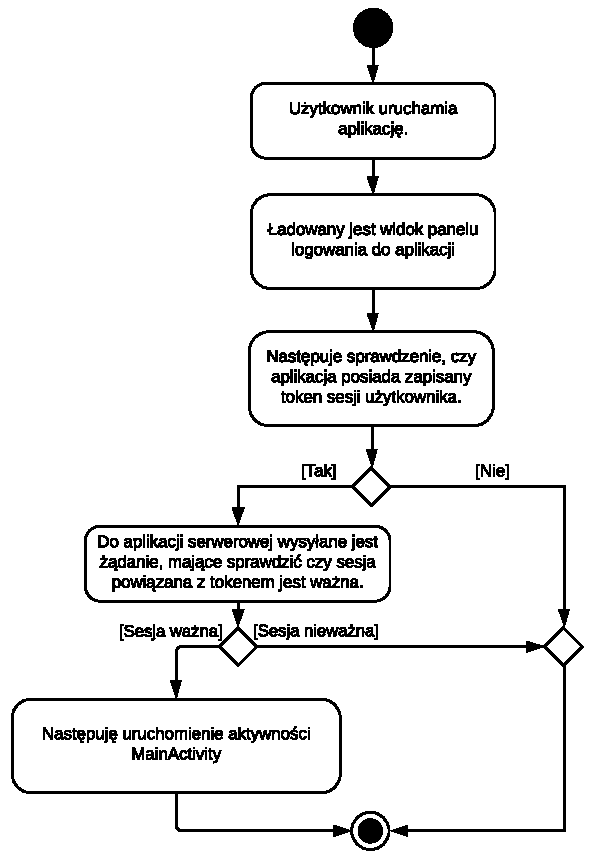
\includegraphics[scale=1]{\ImgPath/rys/diag_aktyw_mob_log_aktyw.pdf}
	\end{center}
	\caption{Diagram aktywności dla LoginActivity.}
	\label{diagramAktywnosciLoginActivity}
\end{figure}
\pagebreak
Ze względu na stosunkową prostotę i jedynie jeden ekran, który należy do tej aktywności, nie została ona podzielona na fragmenty. Inna cechą tej aktywności jest fakt, że nie jest ona zapisywana na stosie cofania, dzięki czemu użytkownik po zalogowaniu, nie jest w stanie cofnąć się do tej aktywności przy użyciu klawisza cofnij.

 Ze względu na fakt wywoływania asynchroniczną naturę metod obsługujących żądania wysyłany do aplikacji serwerowej, klasa LoginActivity implementuje interfejs \textit{LoginObserver} służący do obsługi odpowiedzi na żądania logowania. Został on zaprezentowany na Listingu 5.1.
 \begin{lstlisting}[caption=Interfejs LoginObserver,label=code1,captionpos=b]
interface LoginObserver {
	fun onUserLoginSuccessful(userDTO: UserDTO)  
	fun onUserLoginFailure(errorResponse: ErrorResponse?)
}
 \end{lstlisting} 


Funkcja \textit{onUserLoginSuccessful} zaimplementowana w LoginActivity zostaje wywołana gdy żądanie logowania zostanie pomyślnie zakończone. Jako argument funkcja otrzymuje obiekt transferu danych typu \textit{UserDTO}, który zawiera informacje dotyczące zalogowanego użytkownika oraz żeton sesji, który zostaje zapisany w pamięci urządzenia przy użyciu interfejsu \textit{SharedPreferences}, służącego do przechowywania informacji w postaci klucz--wartość. Funkcja ta odpowiada także za uruchomienie głównej aktywności \textit{MainActivity}

Funkcja \textit{onUserLoginFailure} jest wywoływana w przypadku gdy żądanie logowania zakończy się błędem. Jeśli taka sytuacja wystąpi, funkcja ta wyświetli komunikat użytkownikowi w formie chmurki zwanej tostem(Toast).

\section{MainActivity}
MainActivity jest główną aktywnością w aplikacji składającą się z dwóch fragmentów: 
\begin{enumerate}
	\item PublicationsListFragment -- fragment odpowiedzialny za ekran z listą publikacji użytkownika
	\item UserDetailsFragment -- ekran powiązany z tym fragmentem przedstawia szczegóły zalogowanego użytkownika oraz zezwala na ich edycję.
\end{enumerate}

\subsection{Prezentacja listy publikacji}
Klasa \textit{PublicationsListFragment} jest odpowiedzialna za wyświetlanie ekranu składającego się z przewijanej listy zawierającej odnośniki do poszczególnych publikacji należących do obecnie zalogowanego użytkownika. Za jej wyświetlenie odpowiedzialny jest komponent \textit{RecyclerView}. Jego największą zaletą jest fakt, iż w odróżnieniu od komponentu \textit{ScrollView} jest on w stanie wyświetlać bez większych spowolnień bardzo długie listy. 

Przewaga komponentu \textit{RecyclerView} wynika z faktu, że zamiast trzymać w pamięci wszystkie elementy listy jak ma to miejsce w \textit{ScrollView}, przechowuje jedynie te, które są widoczne na ekranie. W momencie gdy dany element listy znika z pola widzenia, jest przesuwany na początek ze zmienioną zawartością, odpowiadającą kolejnemu elementowi listy. 

Wadą komponentu \textit{RecyclerView} jest niewątpliwe stosunkowo skomplikowana obsługa w kodzie, gdyż aby móc z niego korzystać należy przygotować specjalną klasę będącą adapterem listy wejściowej na jej graficzną reprezentację.

Za pobranie i aktualizację danych odpowiada klasa  \textit{PublicationsListViewModel}, stanowiąca warstwę viewmodelu.
Jej sygnatura została zaprezentowana na Listingu 5.2.

 \begin{lstlisting}[caption=Sygnatura klasy PublicationsListViewModel,label=code1,captionpos=b]
class PublicationsListViewModel : 
	ViewModel(),
	RequestObserver<ArrayList<PublicationListItem>>   
}
\end{lstlisting} 
Klasa \textit{PublicationsListViewModel} dziedziczy po klasie ViewModel, co pozwala w łatwy sposób połączyć ją klasą z warstwy View -- w tym przypadku z klasą \textit{PublicationsListFragment}. Dodatkowo implementuje ona interfejs \textit{RequestObserver}, który umożliwia obsługę odpowiedzi na żądanie. Jest on zbliżony do interfejsu \textit{LoginObserver}, gdyż również posiada on dwie metody: jedną wywoływaną gdy żądanie zakończy się pomyślnie oraz drugą która uruchamiana jest gdy odpowiedź żądania będzie zawierała błąd. Jednak dzięki wprowadzeniu do niego typów generycznych, można go wykorzystywać do obsługi wielu typów odpowiedzi na żądania. Jego kod został zaprezentowany na Listingu 5.3.

 \begin{lstlisting}[caption=Interfejs RequestObserver,label=code1,captionpos=b]
interface RequestObserver<T> {
	fun onSuccess(response: T, type: String)
	fun onFail(errorResponse: ErrorResponse?, type: String)
}
\end{lstlisting} 
 Klasa \textit{PublicationsListViewModel} posiada jedno publiczne pole \textit{publications}, które jest typu \textit{LiveData<List<PublicationListItem>>}. Typ \textit{LiveData} ten daje możliwość obserwacji zmian wartości, dzięki czemu w warstwie widoku wystarczy zdefiniować obserwatora pola typu LiveData, który zostanie poinformowany o każdej zmianie wartości obserwowanego pola i pozwoli na dynamiczne odświeżenie prezentowanych informacji. 
 
 
Na Rysunku 5.2 przedstawione zostało w jaki współpracują między sobą klasy \textit{PublicationsListFragment}, \textit{PublicationsListViewModel}, a także klasa \textit{PublicationRepository}, odpowiedzialna za obsługę żądań dotyczących publikacji. Z uwagi na to, że platforma Android nie pozwala na wykonywanie połączeń sieciowych w sposób synchroniczny wykorzystując główny wąttek, żądanie pobrania informacji o publikacjach jest wywoływane asynchronicznie.
\begin{figure}[!htbp]
	\begin{center}
		\centering
		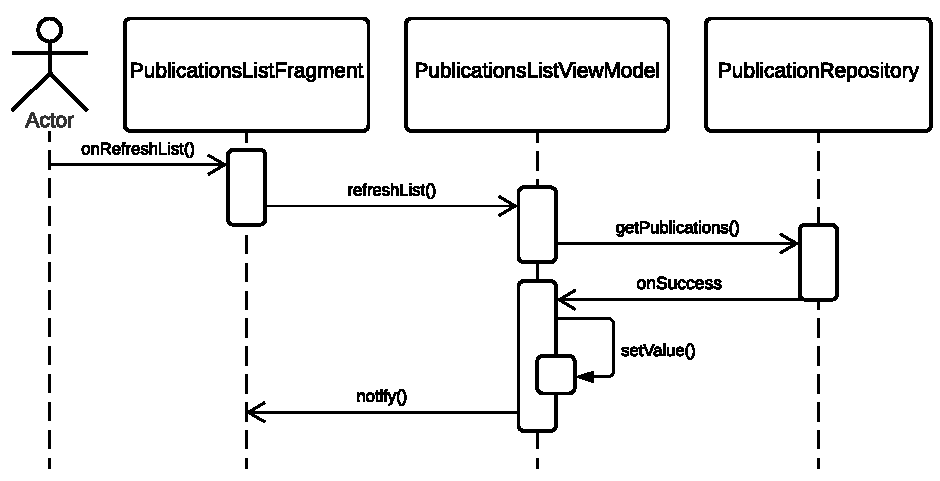
\includegraphics[scale=0.9]{\ImgPath/rys/diag_sek_viewmodel.pdf}
	\end{center}
	\caption{Diagram sekwencji dla ViewModelu.}
	\label{diagramAktywnosciLoginActivity}
\end{figure}

\subsection{Wyświetlanie informacji o użytkowniku}
Klasa \textit{UserDetailsFragment} jest odpowiedzialna za prezentowanie i edycję danych zalogowanego użytkownika. Prezentuje ona na ekranie pola tekstowe zawierające email użytkownika oraz jego pseudonim, a także dwa przyciski odpowiadające za zapisanie zmian oraz wylogowanie użytkownika. W celu aktualizacji danych prezentowanych w warstwie widoku, przygotowana została klasa UserDetailsViewModel.

\section{PublicationDetailsActivity}
\textit{PublicationDetailsActivity} jest aktywnością odpowiedzialna za wyświetlanie, edycję oraz dodawanie pojedynczych publikacji. Wykorzystuje ona jeden fragment o nazwie \textit{PublicationDetailsFragment}, który odpowiedzialny jest za wyświetlanie formularza zawierającego metadane publikacji oraz odnośnik do pliku PDF. 

\subsection{Przełączanie się pomiędzy aktywnościami}
Aktywność \textit{PublicationDetailsActivity} jest zawsze uruchamiana z poziomu aktywności \textit{MainActivity} poprzez wybranie konkretnej publikacji z listy, bądź też w wyniku naciśnięcia na przycisk dodawania nowej publikacji. W systemie Android przełączanie się pomiędzy aktywnościami realizowane jest przy użyciu klasy intencji \textit{Intent}. Zgodnie z dokumentacją \cite{INTENT} jest ona abstrakcyjnym opisem operacji, która powinna zostać wykonana. Dlatego też w celu przełączenia się z jednej aktywności do drugiej, należy podczas tworzenia intencji podać kontekst operacji, w tym przypadku będzie to obecna aktywności oraz klasy aktywności, która ma zostać uruchomiona. Następnie do obiektu intencji można za pomocą metody \textit{putExtra} przekazać wartości, które potem będą mogły być odczytane w uruchamianej aktywności. Na sam koniec należy przekazać nowo utworzony obiektu intencji do metody \textit{startActivity}, co spowoduje uruchomienie nowej aktywności. Cały proces prezentuje Listing 5.4.

\begin{lstlisting}[caption=Przełączanie się pomiędzy aktywnościami,label=code1,captionpos=b]
val intent = Intent(this.activity,
    PublicationDetailsActivity::class.java)
    .apply {
        putExtra(MESSAGE_FROM_LIST_FRAGMENT, message)
    }
startActivity(intent)
    
\end{lstlisting} 

\subsection{Inicjalizacja fragmentu PublicationDetailsFragment}
Ze względu na to, że \textit{PublicationDetailsFragment} jest odpowiedzialna za tworzenie nowych publikacji, ale także za wyświetlanie i edycję już istniejących, w momencie inicjalizacji tego fragmentu, należy odpowiednio dostosować działanie klasy \textit{PublicationDetailsViewModel}, aby była ona świadoma tego czy powinna pobrać wybraną publikację z aplikacji serwerowej, czy też wyświetlić całkowicie pusty formularz. Proces ten przedstawia Rysunek 5.3.

\begin{figure}[!htbp]
	\begin{center}
		\centering
		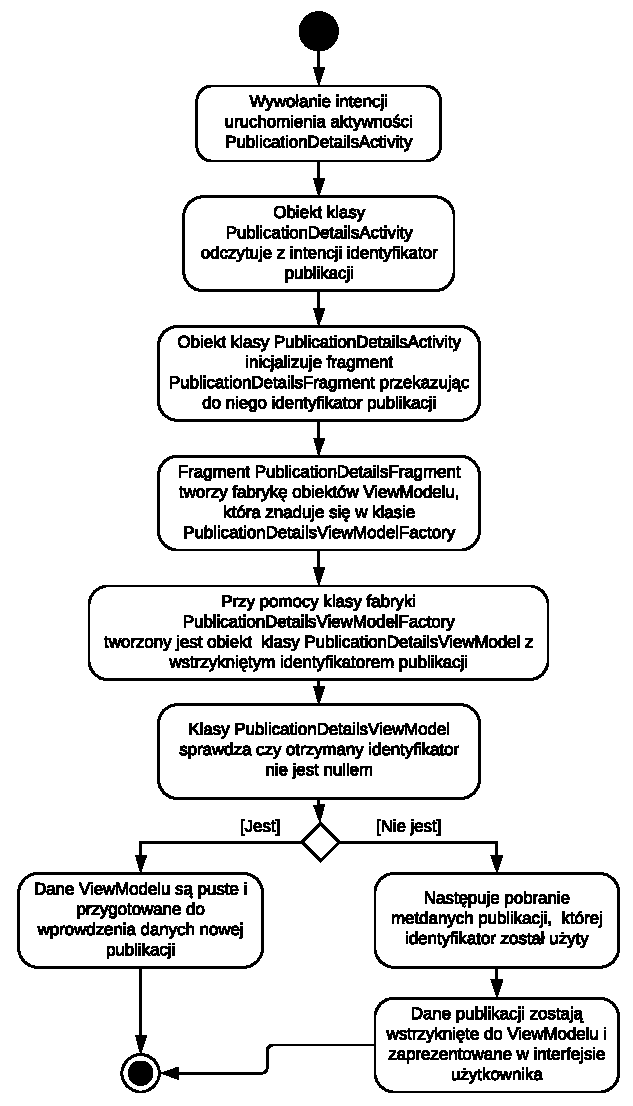
\includegraphics[scale=1]{\ImgPath/rys/diag_aktyw_mob_dod_edyt.pdf}
	\end{center}
	\caption{Proces wyświetlania ekranu ze szczegółami publikacji.}
	\label{diagramAktywnosciMobDodEdyt}
\end{figure}


Aby obiekt klasy \textit{PublicationDetailsViewModel} był świadom jaką publikację należy wyświetlić, należy do niego przekazać identyfikator publikacji. Ze względu na to, że obiekty ViewModelu są uzyskiwane w kodzie przy użyciu klasy \textit{ViewModelProvider}, nie ma możliwości bezpośredniego przekazania parametrów poprzez konstruktor. Dlatego też, przygotowana została dodatkowa klasa \textit{PublicationDetailsViewModelFactory}, która rozszerzając klasę \textit{ViewModelProvider.Factory}, pozwala na przekazywanie odpowiednich parametrów podczas tworzenia obiektów klasy  \textit{PublicationDetailsViewModel}.



\subsection{Wyświetlanie szczegółów publikacji}
Aby wyświetlić szczegóły wybranej publikacji, użytkownik musi nacisnąć na odpowiednią pozycję z listy dostępnej we fragmencie \textit{PublicationsListFragment}, należącym do \textit{MainActivity}.  Następnie dochodzi do uruchomienia aktywności \textit{PublicationDetailsActivity}, wraz z przekazaniem do niej identyfikatora publikacji poprzez intencję. Następnie zgodnie z procesem zawartym na Rysunku 5.4 dochodzi do pobrania danych publikacji oraz ich wyświetlenia w interfejsie.

\subsection{Edycja metadanych publikacji}
W celu edycji publikacji, musi zostać ona najpierw wyświetlona zgodnie z procedurami opisanymi powyżej. Następnie użytkownik edytuje wybrane metadane, po czym naciska na przycisk \textit{Save}, co powoduje wysłanie żądanie edycji publikacji.

\subsection{Dodanie nowej publikacji}
Proces tworzenia nowej publikacji rozpoczyna się od naciśnięcia przez użytkownika przycisku dodawania publikacji we fragmencie \textit{PublicationsListFragment}, należącym do \textit{MainActivity}, które to powoduje uruchomienie aktywności \textit{PublicationDetailsActivity}. Jednakże w odróżnieniu od procesu wyświetlania, do intencji nie trafia identyfikator żadnej publikacji. Skutkuje to innym zachowaniem klasy \textit{PublicationDetailsViewModel}, która nie pobiera danych żadnej publikacji, inicjalizując jedynie dane ViewModelu bez wprowadzania żadnych wartości. 

Następnie użytkownik dodaje za pomocą przycisku \textit{Select PDF}, wybiera z pamięci telefonu plik PDF zawierający publikację. Plik zostaje przesłany do aplikacji serwerowej w celu przetworzenia. Kiedy serwer zwróci odczytane informacje zostaję wprowadzone do ViewModelu i automatycznie są wyświetlane użytkownikowi, który może teraz dokonać ich uzupełnienia. Następnie użytkownik naciska na przycisk \textit{Save} co powoduje wysłanie żądania dodania nowej publikacji. Proces przedstawiony został na Rysunku 5.5.

\begin{figure}[!htbp]
	\begin{center}
		\centering
		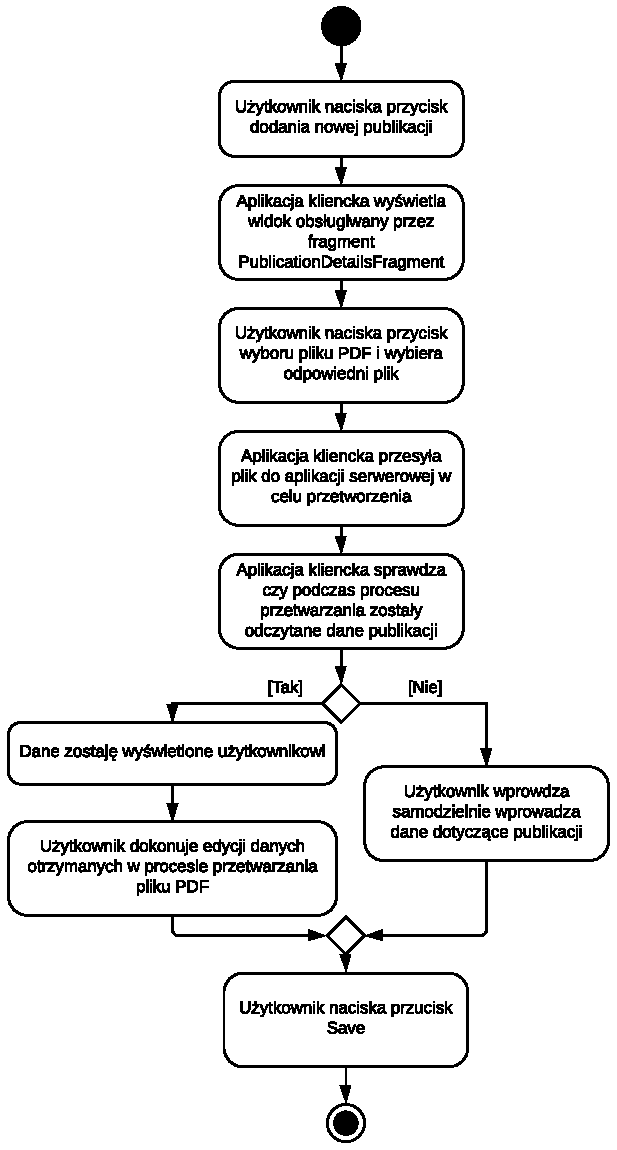
\includegraphics[scale=0.893]{\ImgPath/rys/diag_aktyw_mob_dodawanie_pub.pdf}
	\end{center}
	\caption{Proces dodawania nowej publikacji z poziomu aplikacji klienckiej.}
	\label{diagramAktywnosciMobDodEdyt}
\end{figure}



\chapter{Testy}
Przed przekazaniem aplikacji użytkownikom, należy wykonać przeprowadzić testy. Mają one na celu zminimalizować ryzyko wystąpienia niepożądanych sytuacji podczas korzystania z aplikacji, powinna ona przejść testy sprawdzające wszystkie funkcje i sytuacje wyjątkowe, które powinny zostać obsłużone przez aplikację. Dlatego też cały system został poddany różnorodnym testom w celu sprawdzenia następujących funkcji: 

\begin{enumerate}
	\item Logowanie i wylogowanie;
	\item Przetwarzanie plików PDF
	\item Dodawanie, edycja i usuwanie publikacji.
\end{enumerate}

Dla każdej z funkcji zostanie przeprowadzone kilka testów, aby sprawdzić jak dana funkcja zachowuje się w przypadku gdy wszystko dzieje się zgodnie z założeniami, ale także jak obsługiwane są sytuacje mniej spodziewane oraz błędy. 

\section{Rejestracja, logowania i wylogowanie}
Test funkcji rejestracji wymaga utworzenia konta użytkownika, a następnie zalogowania przy użyciu tego konta, przez co testy logowania, zostały wykorzystane w celu zweryfikowania efektów rejestracji.  

Dla funkcji logowania zostaną przeprowadzone testy przy użyciu poprawnych danych logowania, które powinny pozwolić na zalogowanie użytkownika ale także takich, które zawierają niepoprawny adres email (Test ten jest częścią testu rejestracji) lub hasło. Oprócz tego sprawdzone zostało czy aplikacja poprawnie obsługuje sytuację gdy użytkownik otwiera aplikację, do której zalogował się wcześniej.


\pagebreak


\subsection{Próba logowania na nieistniejące konto}
Na Rysunku 6.1 zostało przedstawione zachowanie aplikacji w przypadku, próby zalogowania się za pomocą adresu email \textit{pje@test.co}, do którego nie jest przypisany żaden użytkownik. Zgodnie z oczekiwaniami logowanie zakończyło się błędem, mówiącym o braku konta powiązanego z danym adresem email. Treść tego błędu została wyświetlona użytkownikowi, w formie komunikatu typu Toast.
\begin{figure}[!htbp]
	\begin{center}
		\centering
		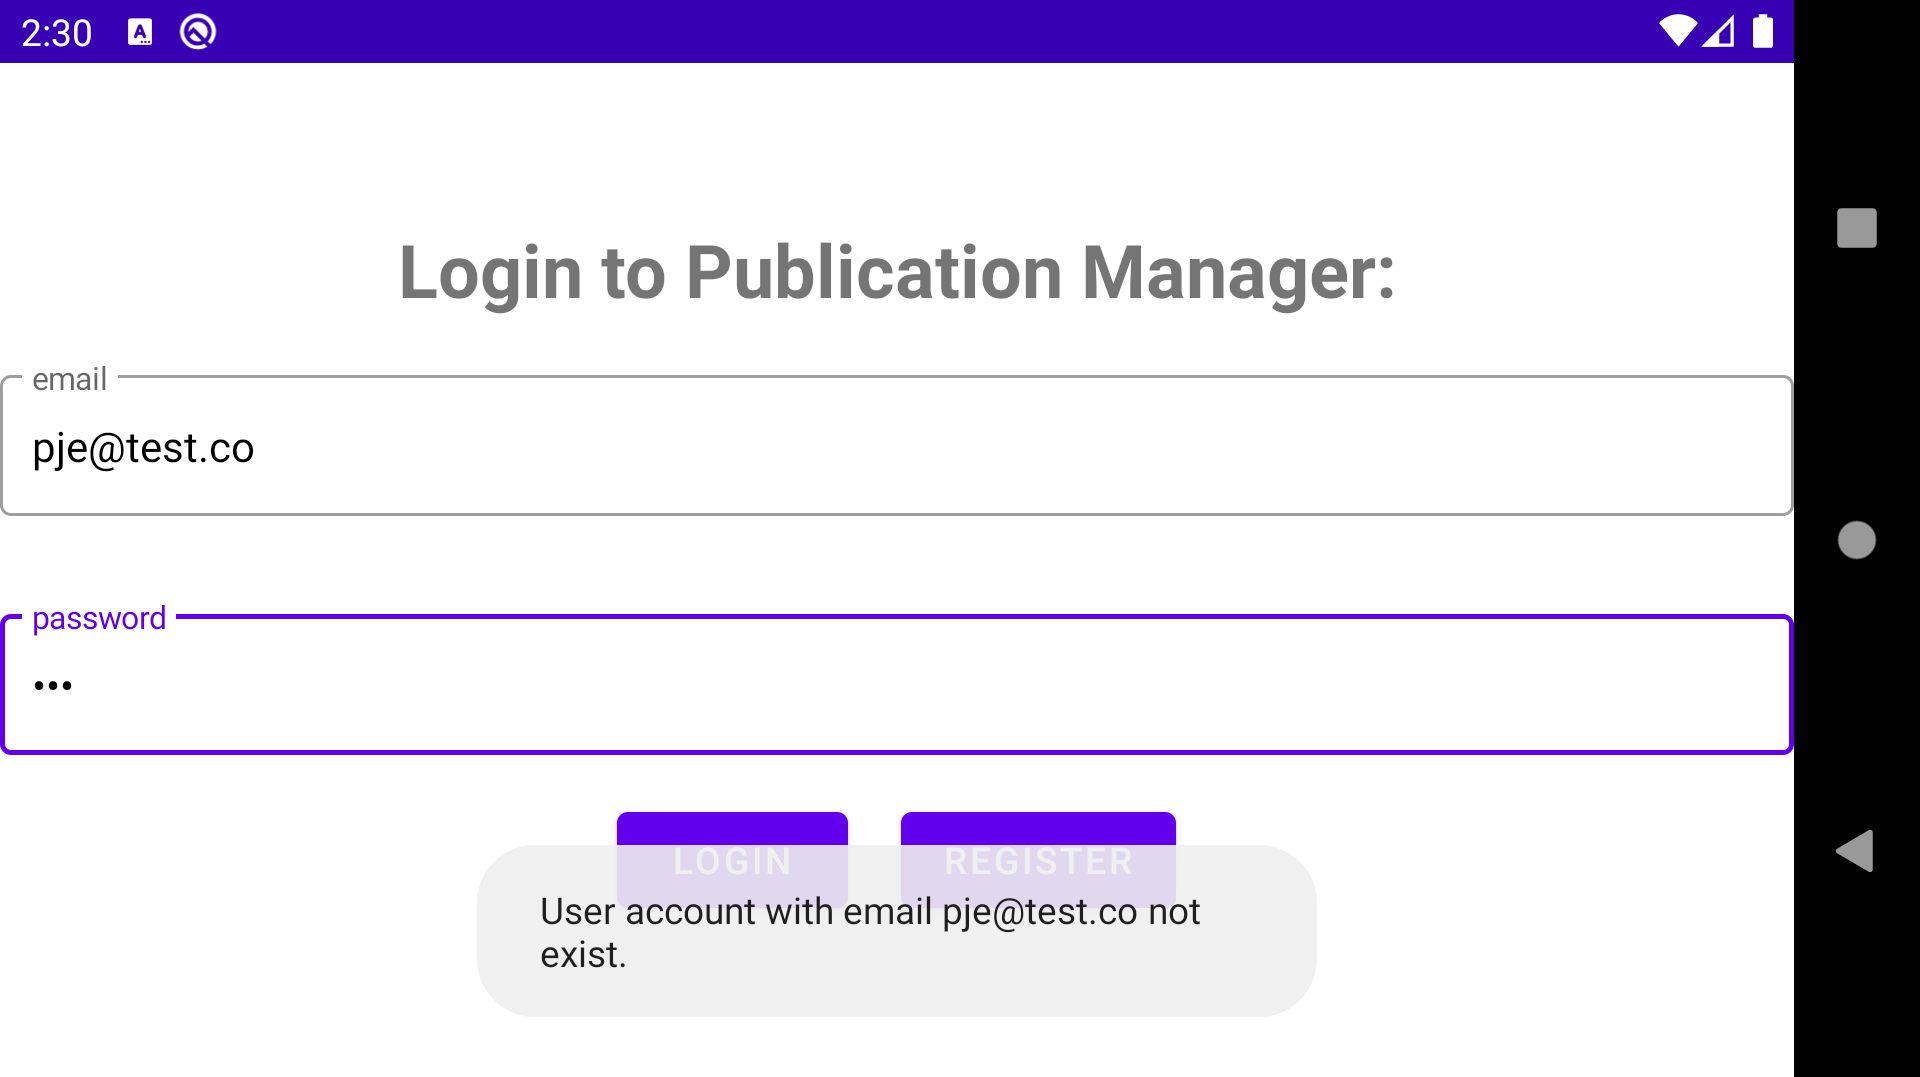
\includegraphics[scale=0.27]{\ImgPath/rys/screenshots/email-not-exist.png}
	\end{center}
	\caption{Logowanie na nieistniejące konto.}
	\label{zrzutLogowaniePoprawne}
\end{figure}

\subsection{Próba zalogowania przy użyciu błędnego hasła}
Rysunek 6.2  przedstawiona zachowanie aplikacji w przypadku, próby zalogowania się za pomocą adresu email, który jest przypisany do jednego z użytkowników oraz hasła, które jednak nie jest prawidłowym hasłem tego użytkownika. Zgodnie z oczekiwaniami logowanie zakończyło się błędem, mówiącym niepoprawnym haśle. Treść tego błędu została wyświetlona użytkownikowi, w formie komunikatu typu Toast.

\pagebreak

\begin{figure}[!htbp]
	\begin{center}
		\centering
		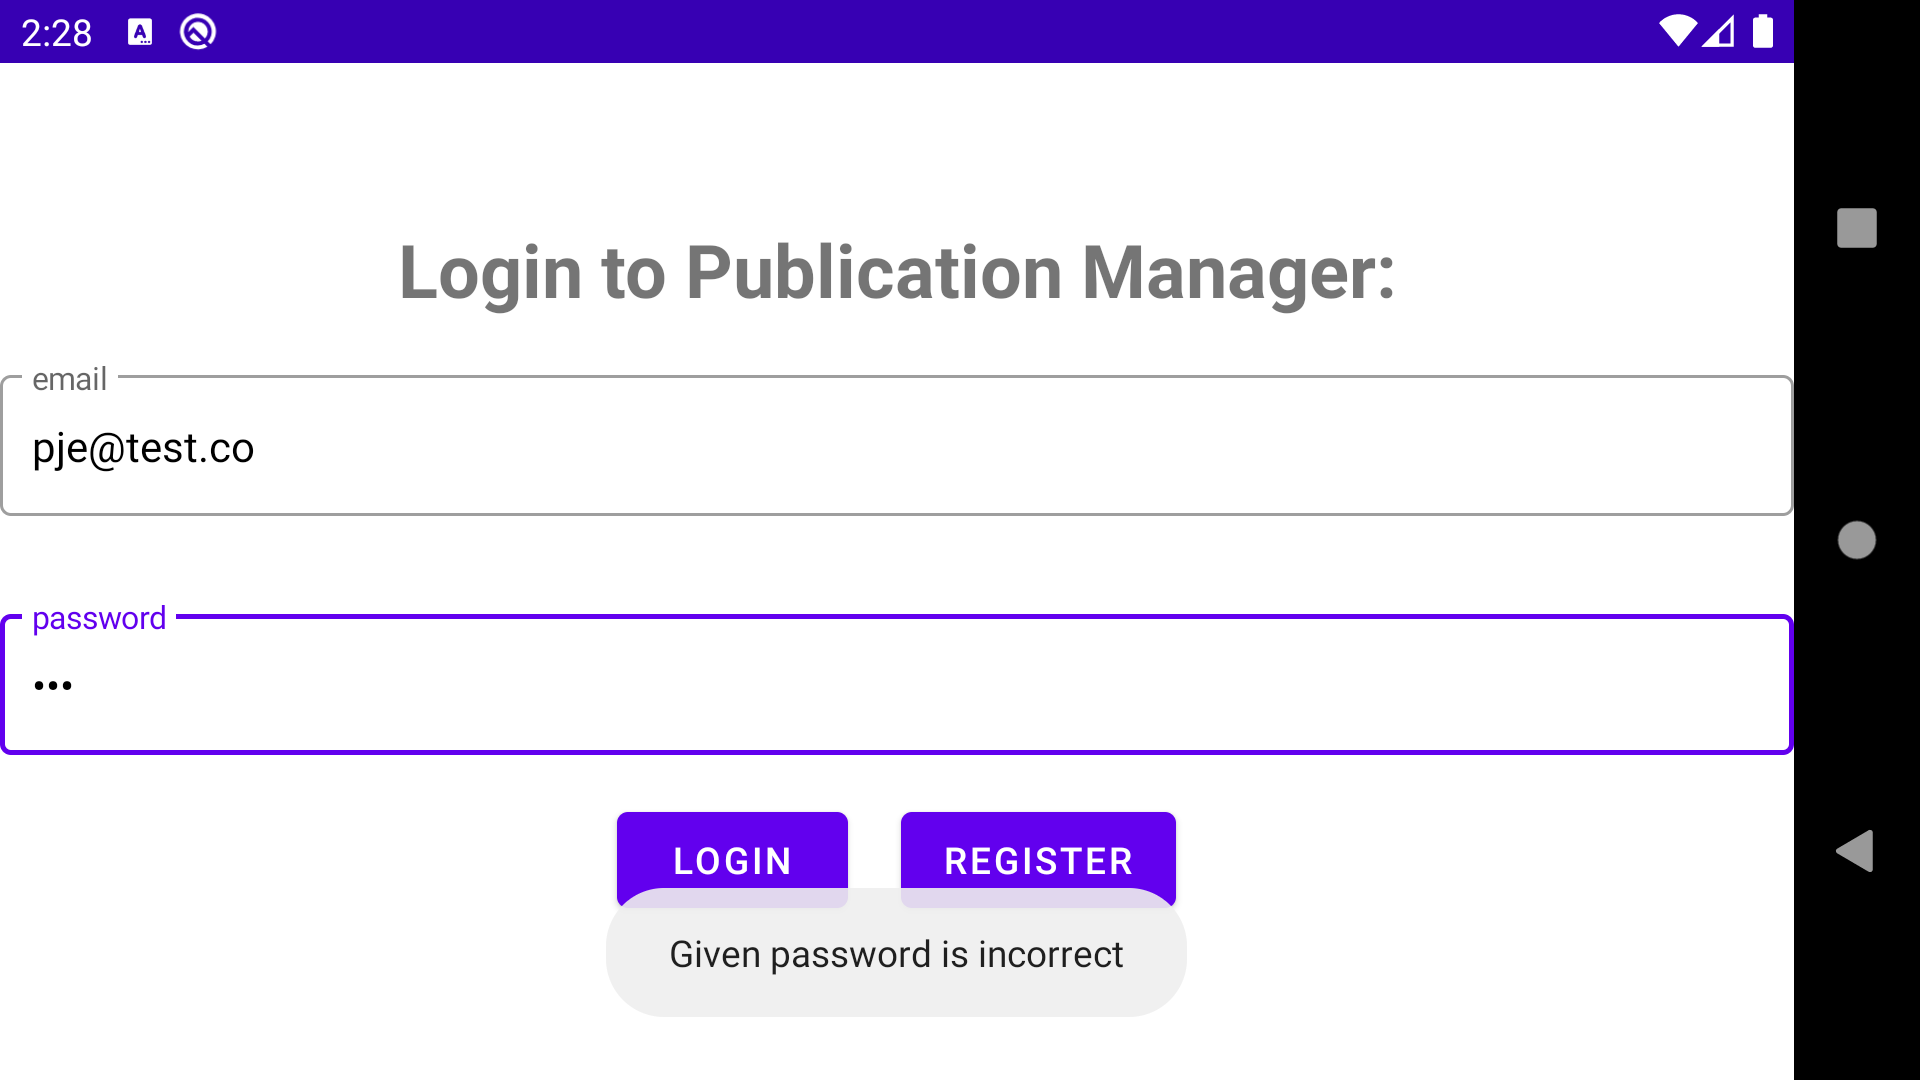
\includegraphics[scale=0.2]{\ImgPath/rys/screenshots/password-incorrect.png}
	\end{center}
	\caption{Logowanie przy użyciu niepoprawnego hasła.}
	\label{zrzutLogowaniePoprawne}
\end{figure}

\begin{figure}[!htbp]
	\begin{center}
		\centering
		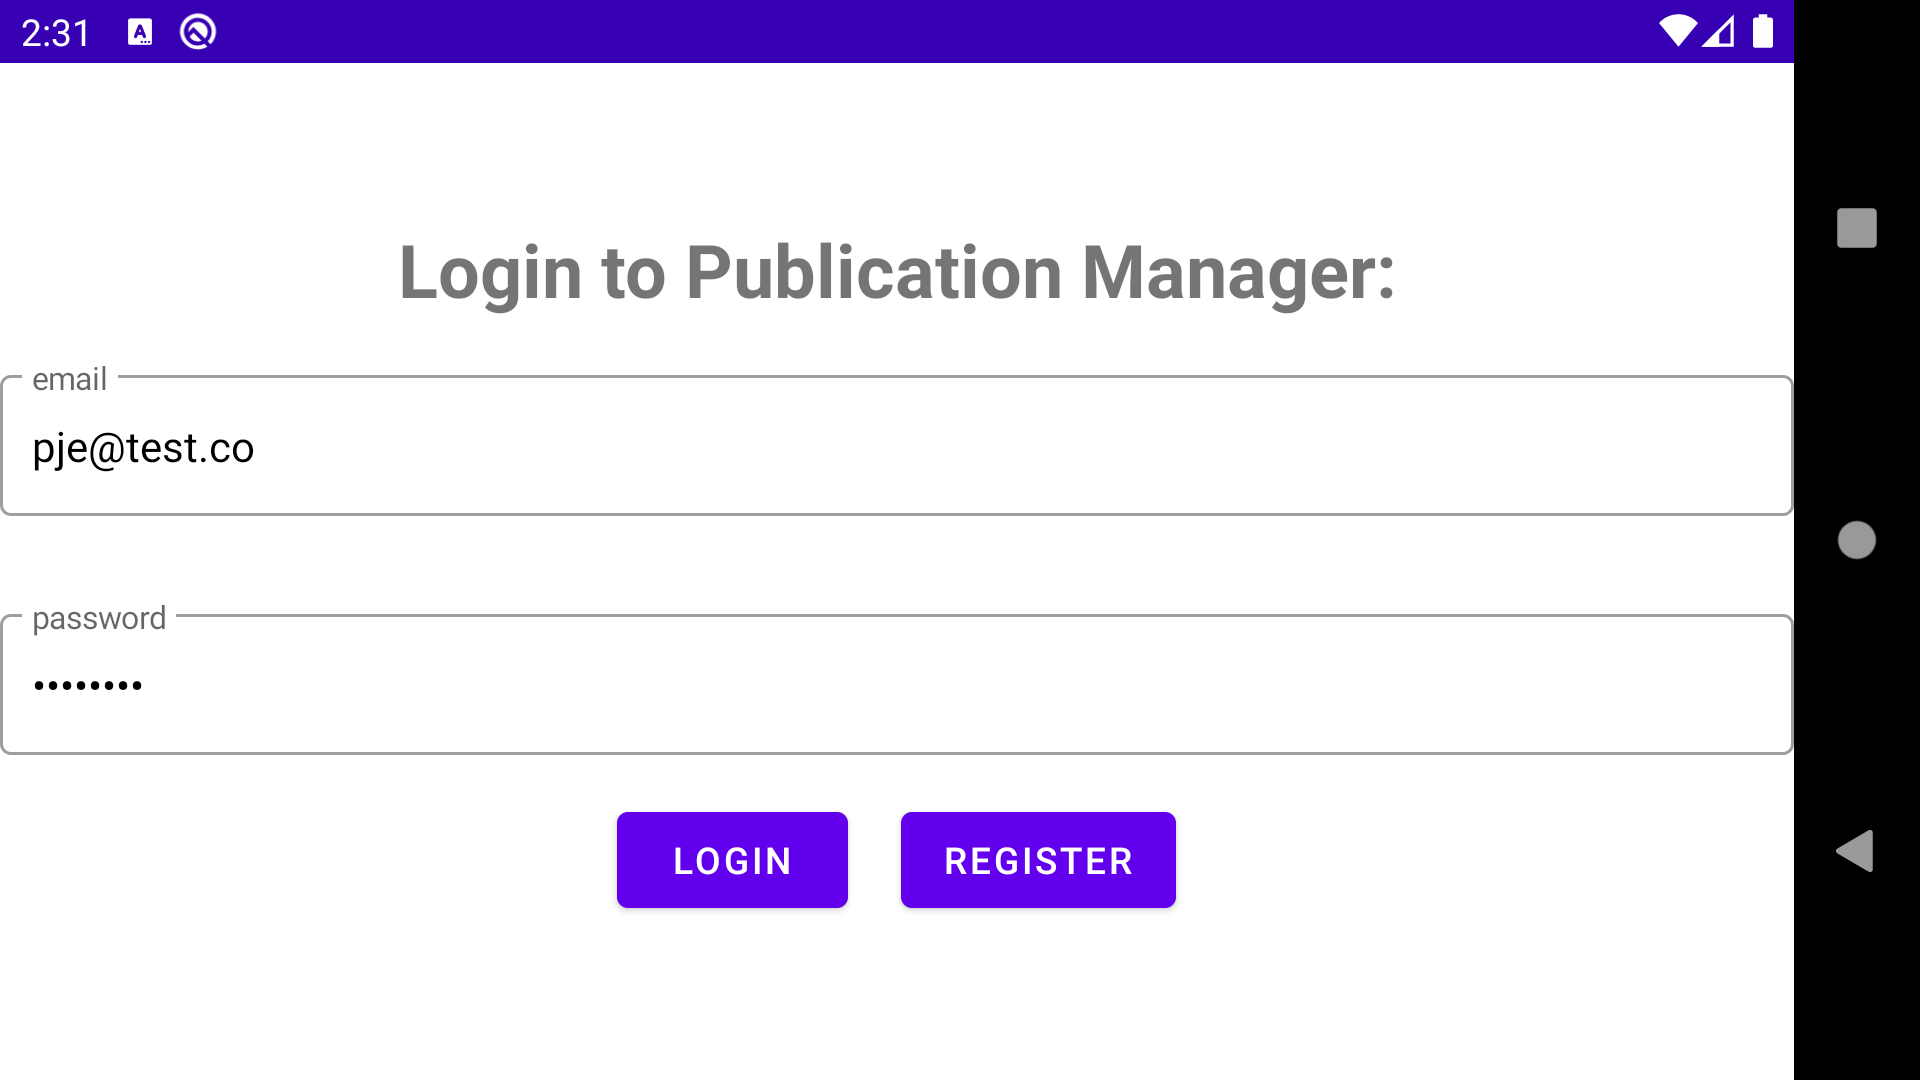
\includegraphics[scale=0.2]{\ImgPath/rys/screenshots/login.png}
	\end{center}
	\caption{Logowanie prawidłowe.}
	\label{zrzutLogowaniePoprawne}
\end{figure}


\subsection{Próba zalogowania na nowo utworzone konto}
Rysunek 6.3  przedstawiona zachowanie aplikacji w przypadku, próby zalogowania się za pomocą danych logowania, to jest adresu email oraz hasła które są przypisany do nowo utworzonego konta użytkownika. Zgodnie z oczekiwaniami logowanie zakończyło się sukcesem, w efekcie czego, aplikacja wyświetliła ekran z listą publikacji(przedstawiony na Rysunku 6.4) należących do użytkownika, który właśnie się zalogował. 




\begin{figure}[!htbp]
	\begin{center}
		\centering
		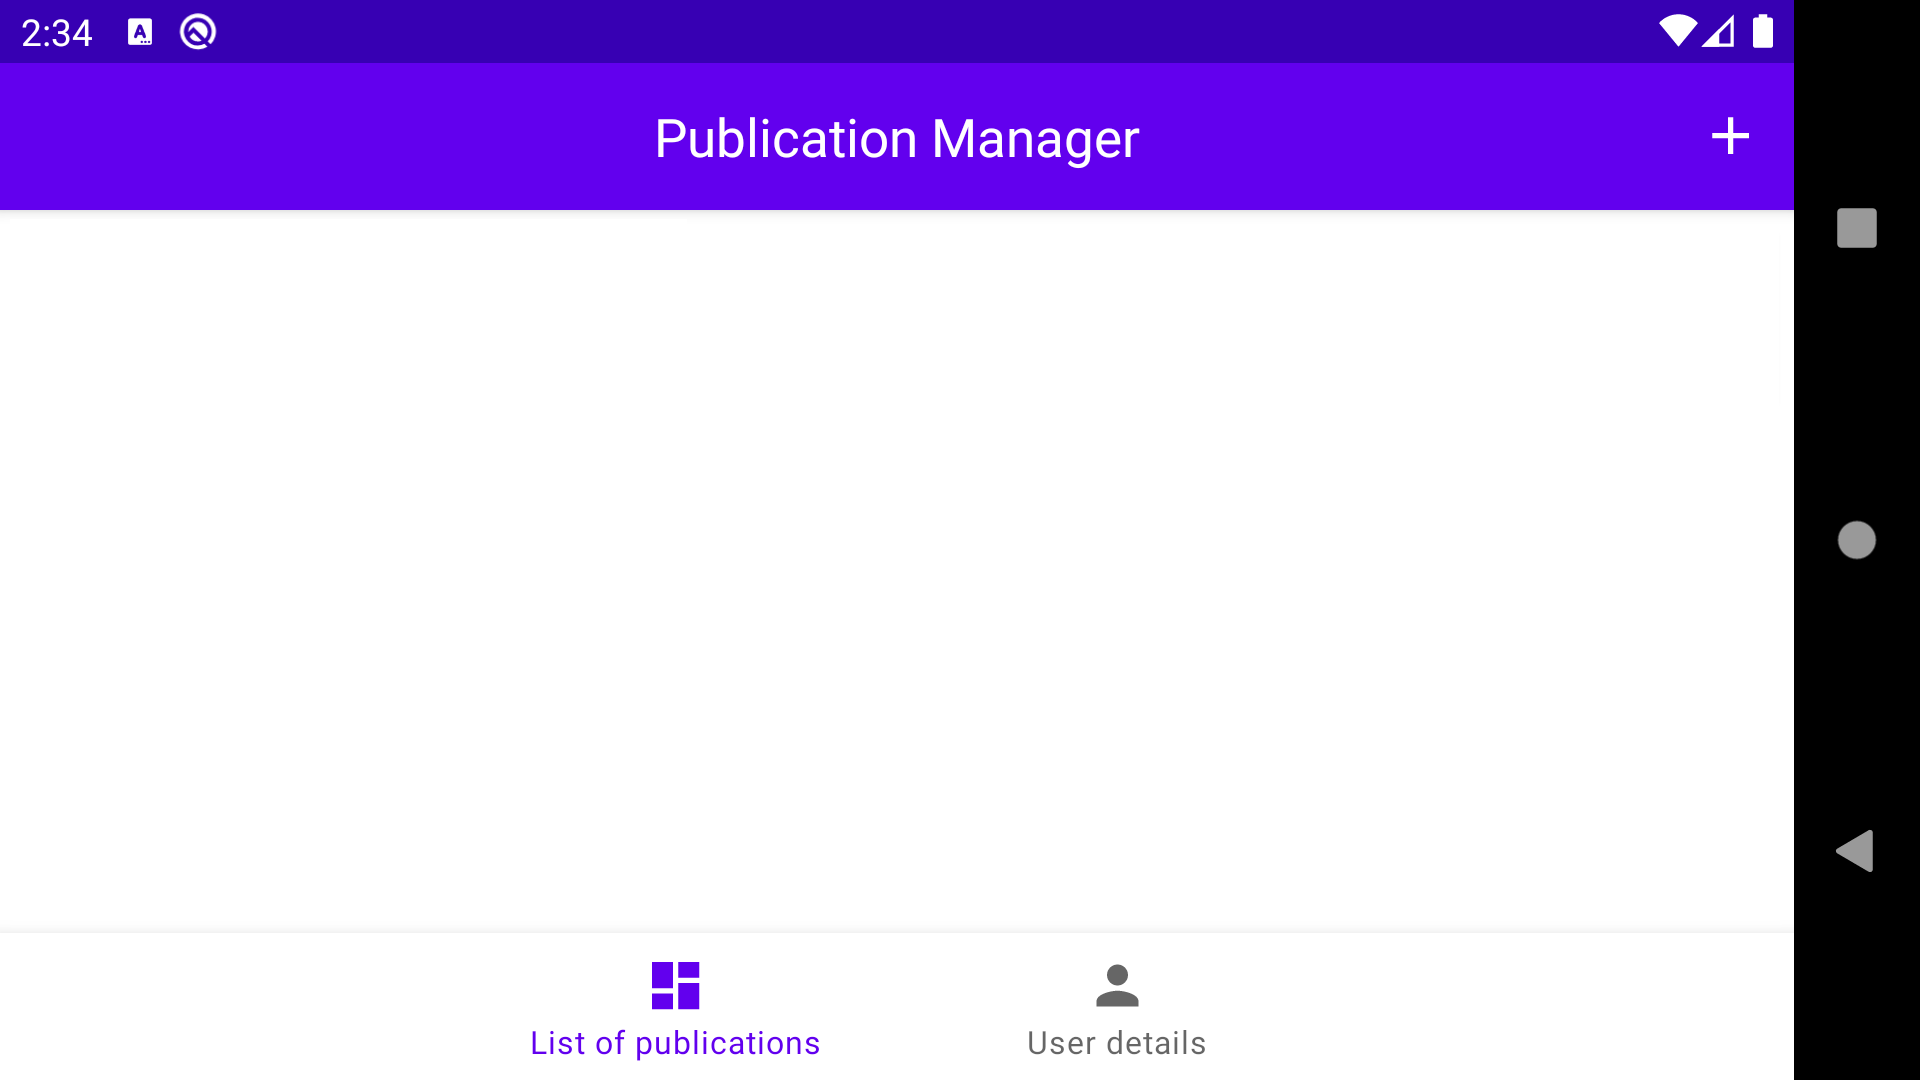
\includegraphics[scale=0.27]{\ImgPath/rys/screenshots/after-login.png}
	\end{center}
	\caption{Lista publikacji użytkownika, wyświetlona po zalogowaniu.}
	\label{diagramAktywnosciMobDodEdyt}
\end{figure}

\subsection{Wylogowanie}
Na Rysunku 6.5 został przedstawiony ekran zawierający szczegóły dotyczące zalogowanego użytkownika, na którym znajduje się także przycisk umożliwiający wylogowanie. Po jego naciśnięciu użytkownik, zgodnie z oczekiwaniami, został przekierowany do ekranu logowania(przedstawiony na Rysunku 6.6). Nie możliwy jest także powrót do ekranu szczegółów użytkownika poprzez naciśnięcie klawisza powrotu. Również po ponownym otwarciu aplikacji użytkownik został przeniesiony nie do listy publikacji a do ekranu logowania, co oznacza że został poprawnie wylogowany.


\begin{figure}[!htbp]
	\begin{center}
		\centering
		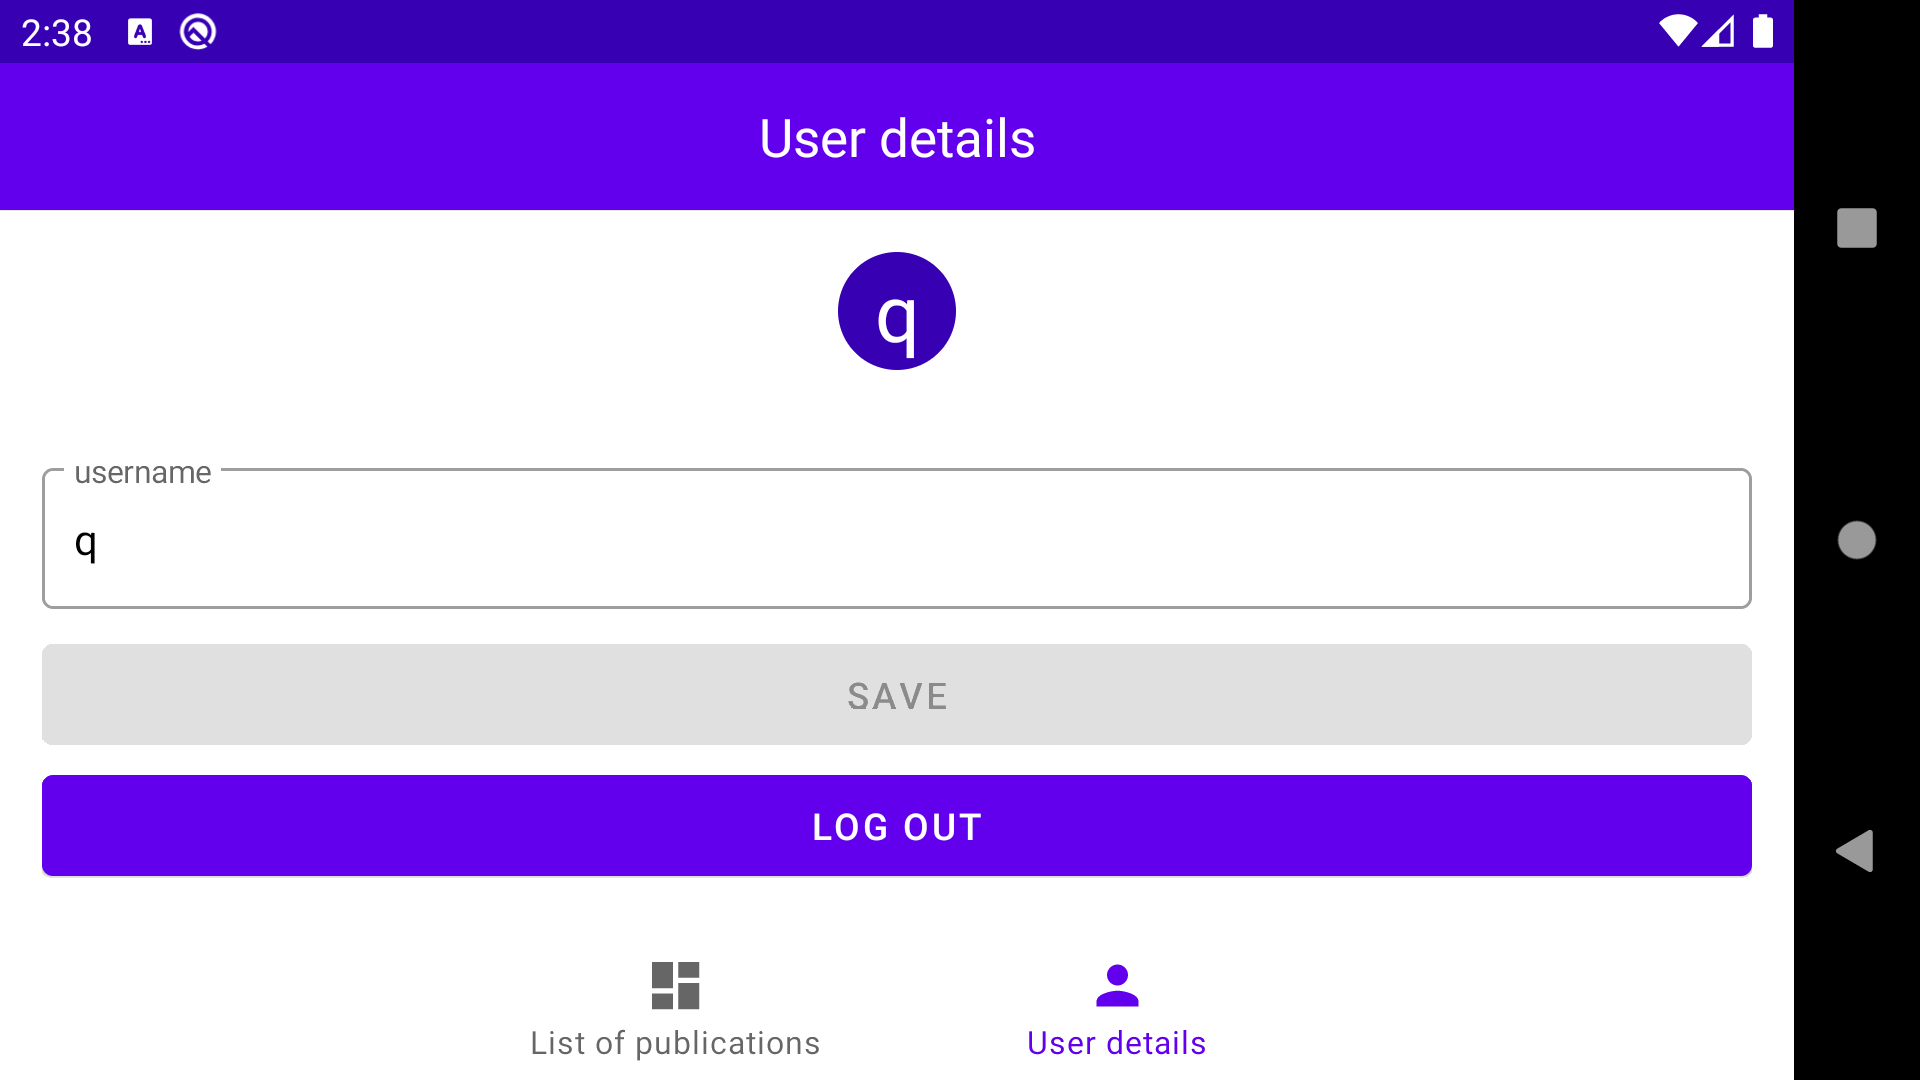
\includegraphics[scale=0.27]{\ImgPath/rys/screenshots/before-logout.png}
	\end{center}
	\caption{Ekran szczegółów użytkownika z przyciskiem wylogowania.}
	\label{zrzutLogowanieEkranUserDetails}
\end{figure}


\pagebreak


\begin{figure}[!htbp]
	\begin{center}
		\centering
		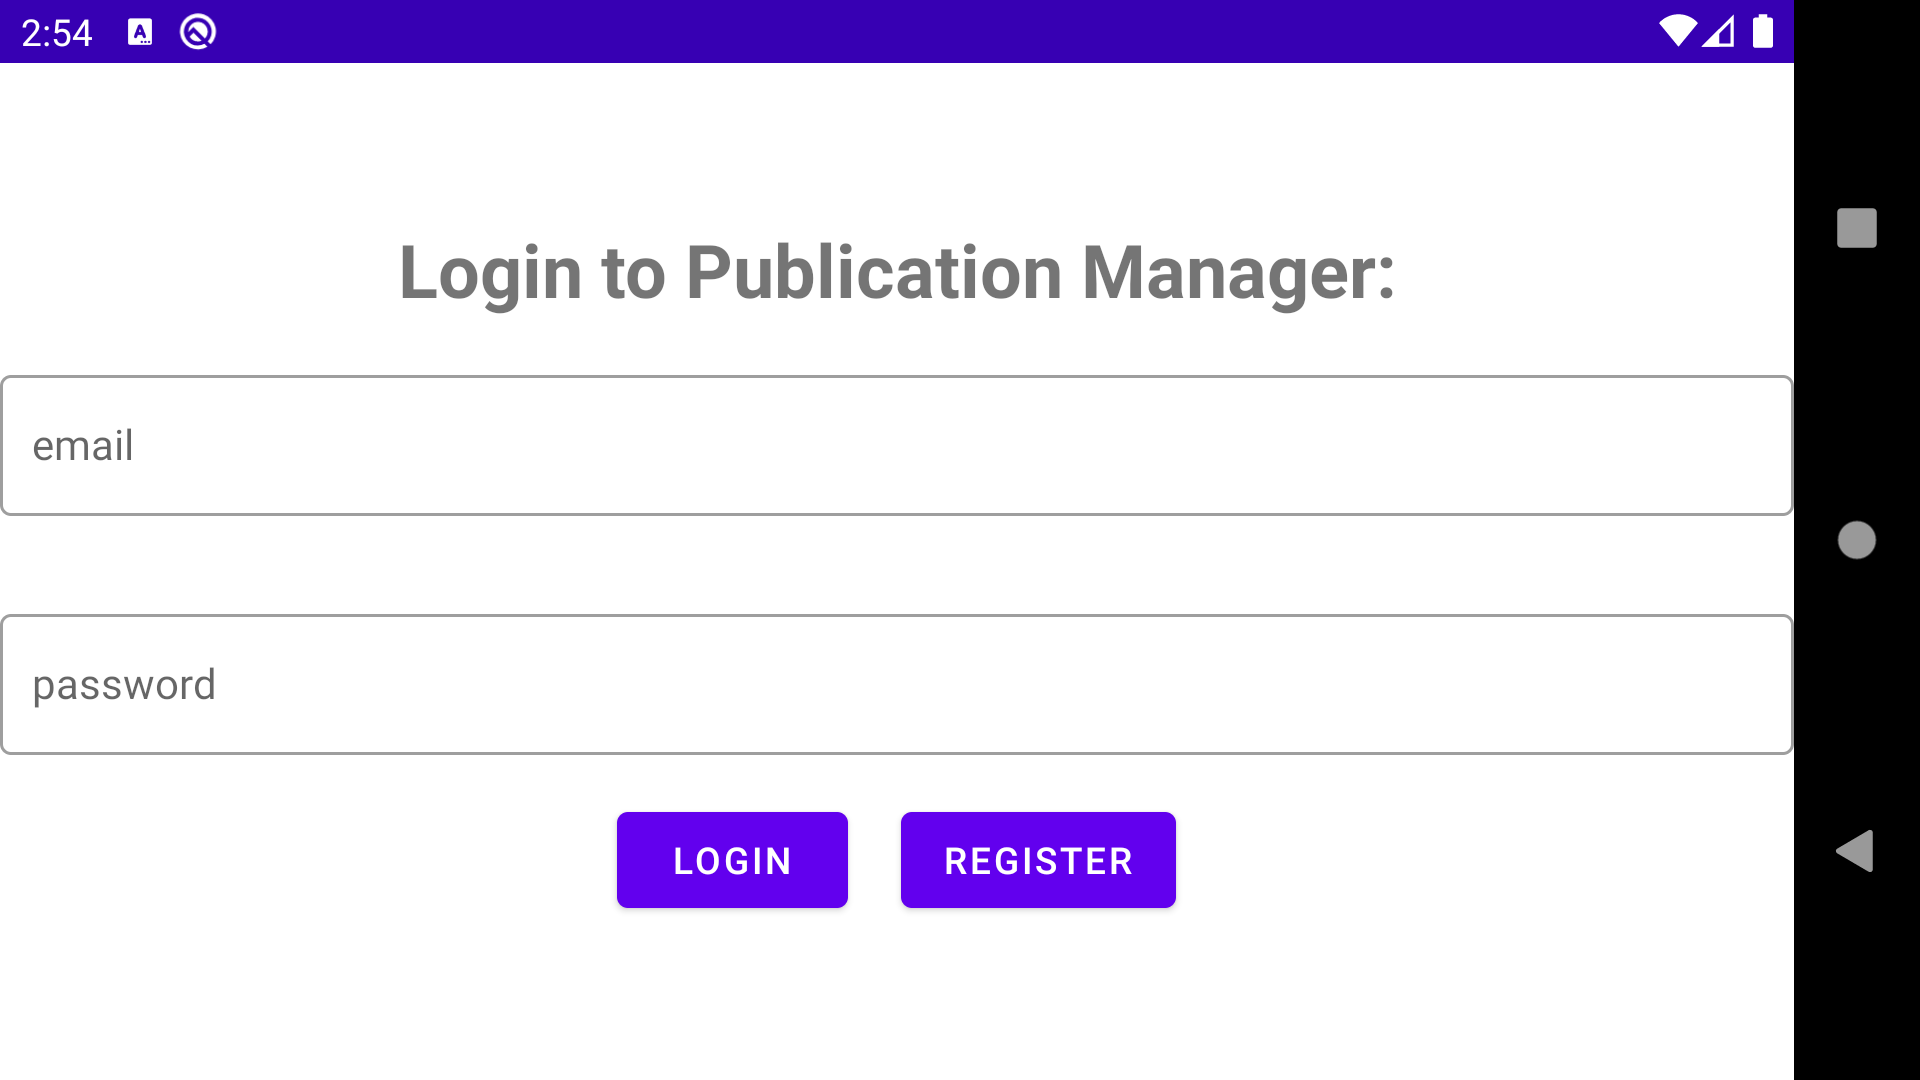
\includegraphics[scale=0.2]{\ImgPath/rys/screenshots/logout.png}
	\end{center}
	\caption{Ekran logowania wyświetlony po poprawnym wylogowaniu.}
	\label{zrzutLogowaniePoWylogowaniu}
\end{figure}

\subsection{Ponowne otwarcie aplikacji po wcześniejszym zalogowaniu}
W przypadku gdy użytkownik zalogował się, zamknął aplikację, a następnie otworzył ją ponownie przed upływem ważności sesji(w tym przypadku okres ten wynosi tydzień), aplikacja nie powinna wymagać ponownego logowania, tylko przynieść użytkownika, po wcześniejszym zweryfikowaniu ważności sesji do ekrany listy publikacji, który został przedstawiony na Rysunku 6.4. Test odzwierciedlający powyższy proces został przeprowadzony i jego wynik jest zgodny z oczekiwaniami.

\section{Przetwarzanie plików PDF}
W tej sekcji zostaną przedstawione wyniki testów aplikacji, polegających na sprawdzeniu poprawności działania przetwarzania plików PDF. Do tego celu wykorzystane zostaną pliki o następujących cechach:
\begin{enumerate}
	\item Plik zawierający w metadanych pliku informacje takie jak tytuł oraz autorzy ale także numer DOI;
	\item Plik zawierający numer DOI wewnątrz treści pliku;
	\item Plik zawierający w metadanych pliku tylko tytuł oraz autorów;
	\item Plik nie zawierający żadnych metadanych oraz numeru DOI.
\end{enumerate}

\subsection{Plik zawierający w metadanych pliku informacje takie jak tytuł oraz autorzy ale także numer DOI}
Efekt przetwarzania pliku PDF oparta o identyfikator DOI oraz pozostałe informacje zawarte w metadanych został przedstawiony na Rysunku 6.7. Ekran zawierający szczegóły publikacji prezentuje dane uzyskane z bazy danych DOI oraz bezpośrednio w pliku -- tytuł publikacji został ustalony na podstawie API\footnote{Adres API: \url{https://api.crossref.org/works/}} zezwalającego na pobieranie informacji na temat publikacji na podstawie DOI, natomiast autor został odczytany bezpośrednio z metadanych pliku PDF. Obie te wartości zgadzają się z informacjami zawartymi w treści pliku.

\begin{figure}[!htbp]
	\begin{center}
		\centering
		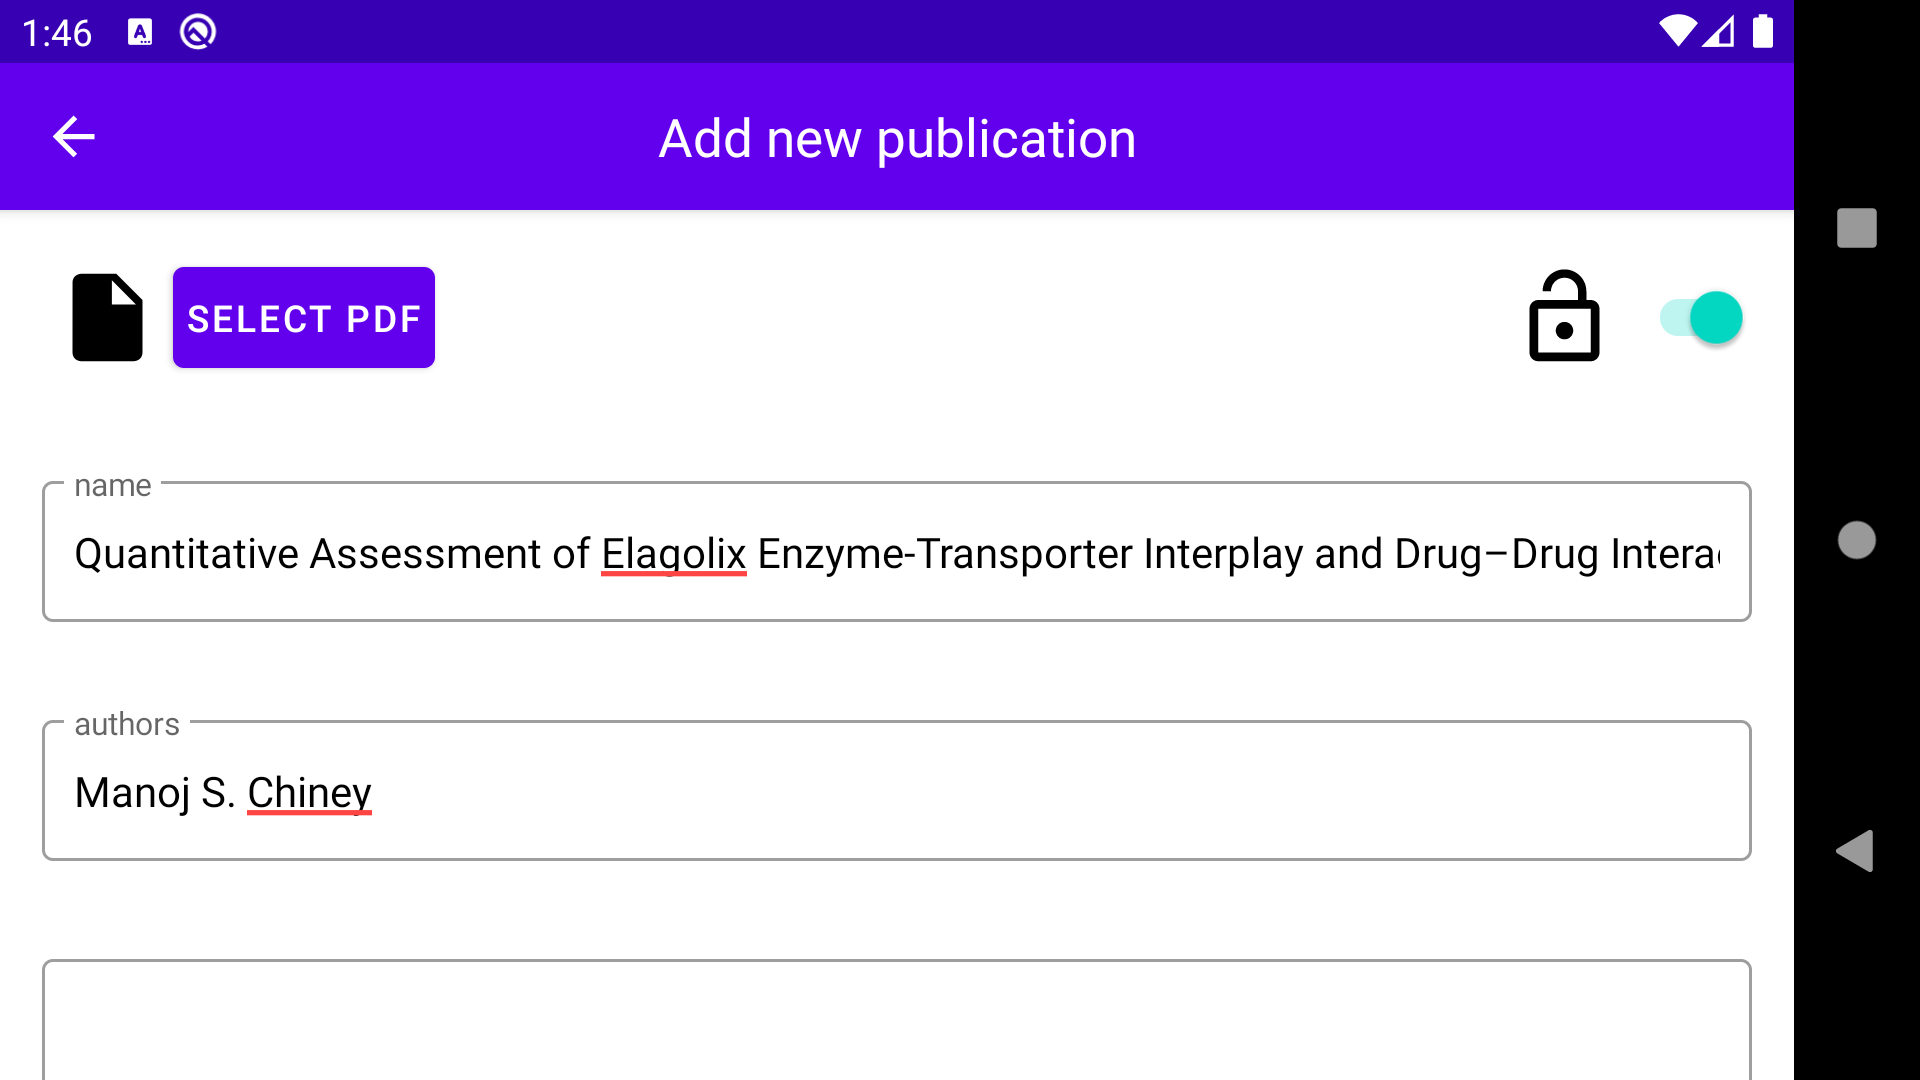
\includegraphics[scale=0.2]{\ImgPath/rys/screenshots/title_auth_doi_metadata.png}
	\end{center}
	\caption{Ekran szczegółów publikacji po przetworzeniu dokumentu z DOI i metadanymi.}
	\label{zrzutPrzetwarzanieFull}
\end{figure}

\pagebreak

\subsection{Plik zawierający numer DOI wewnątrz treści pliku}
Rysunek 6.8  przedstawia ekran zawierający szczegóły publikacji odczytane z pliku PDF zawierającego identyfikator DOI w treści pliku, ale nie posiadającym żadnych dodatkowych informacji w metadanych pliku. Proces odczytywania tytułu przebiegł pomyślnie, gdyż jest zgodny z tytułem publikacji zawartej wewnątrz pliku, który brzmi: \textit{,,Revision of the instructions to authors to require a structured
abstract, digital object identifier of each reference, and author’s
voice recording may increase journal access''}.


\begin{figure}[!htbp]
	\begin{center}
		\centering
		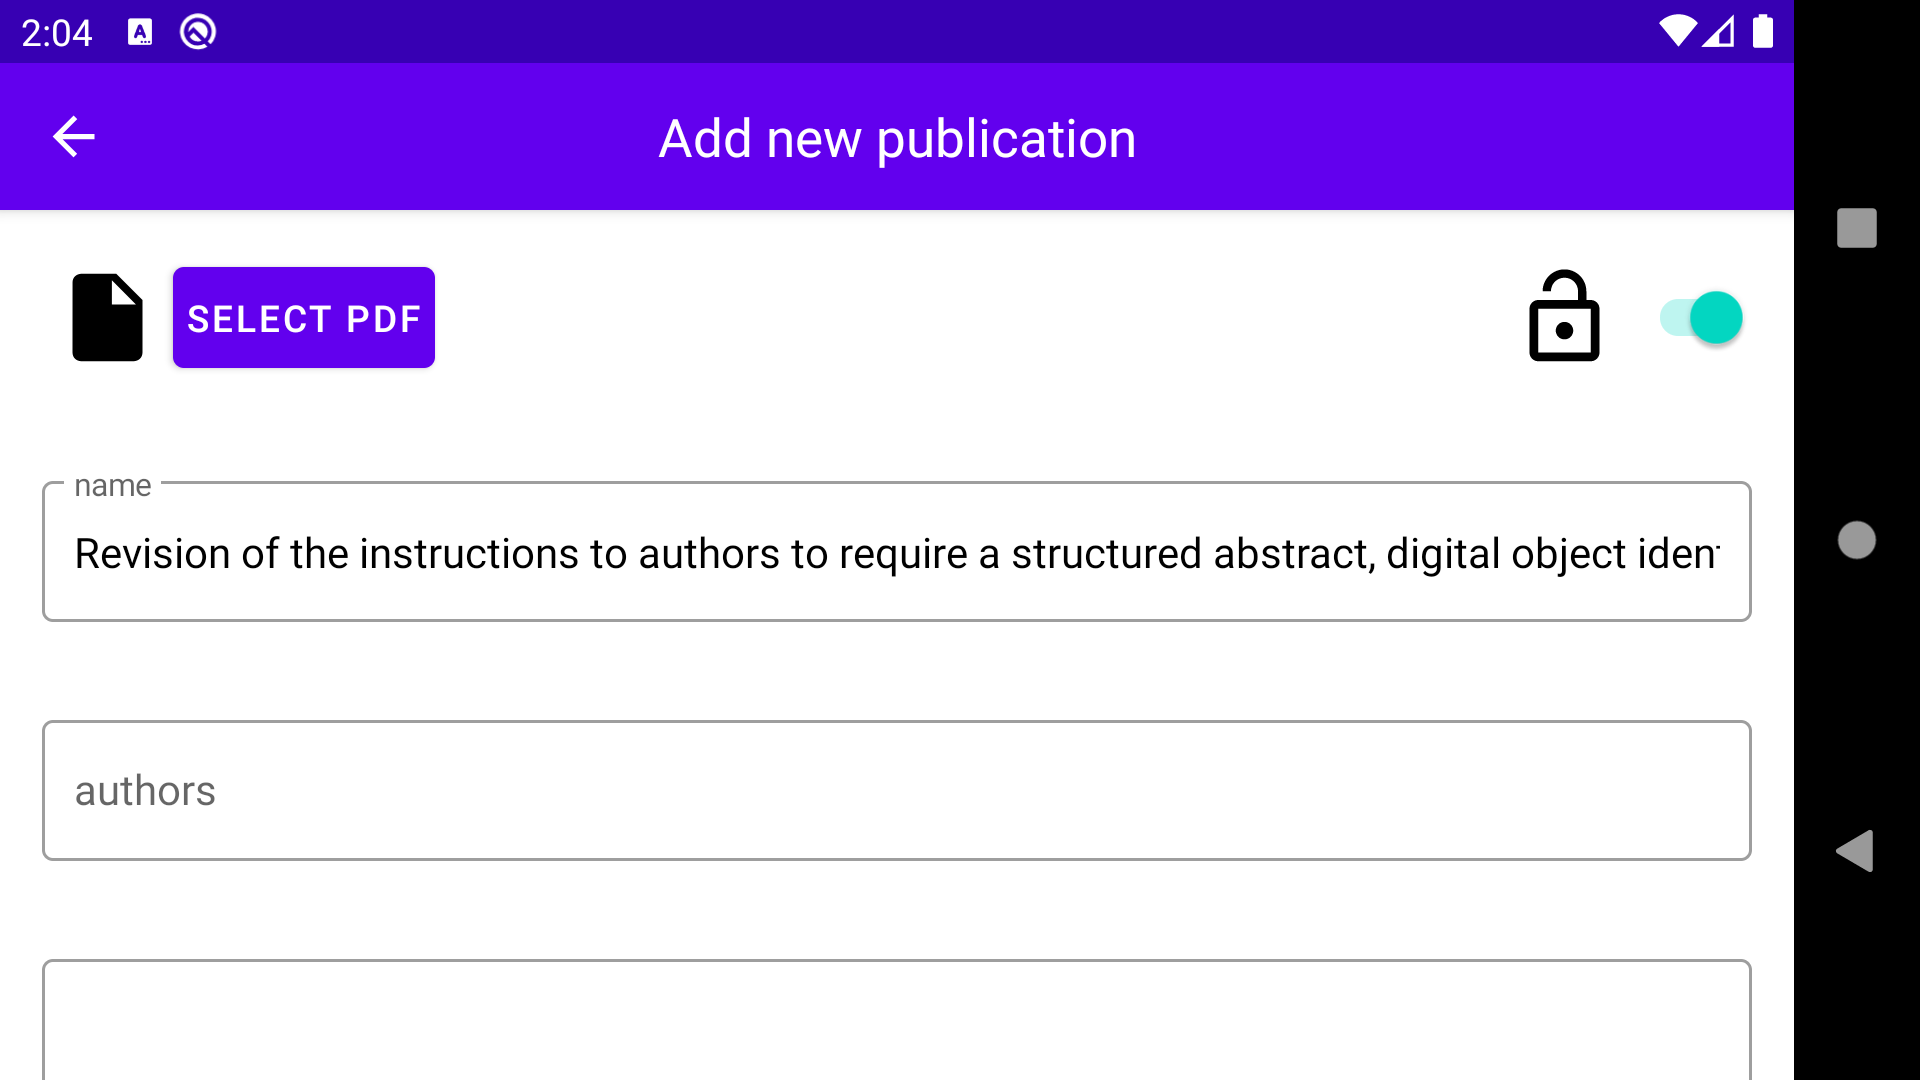
\includegraphics[scale=0.2]{\ImgPath/rys/screenshots/doi_text.png}
	\end{center}
	\caption{Ekran szczegółów publikacji po przetworzeniu dokumentu zawierającego DOI w tekście pliku.}
	\label{zrzutPrzetwarzanieDOIText}
\end{figure}

\subsection{Plik zawierający w metadanych pliku tylko tytuł oraz autorów}
Rysunek 6.9 przedstawiona ekran zawierający szczegóły publikacji odczytane z pliku PDF nie posiadającego DOI, a jedynie metadane w postaci tytułu i autorów. Plik który został użyty w teście zawiera rozkład jazdy pociągów PKP dla stacji Suwałki.




\begin{figure}[!htbp]
	\begin{center}
		\centering
		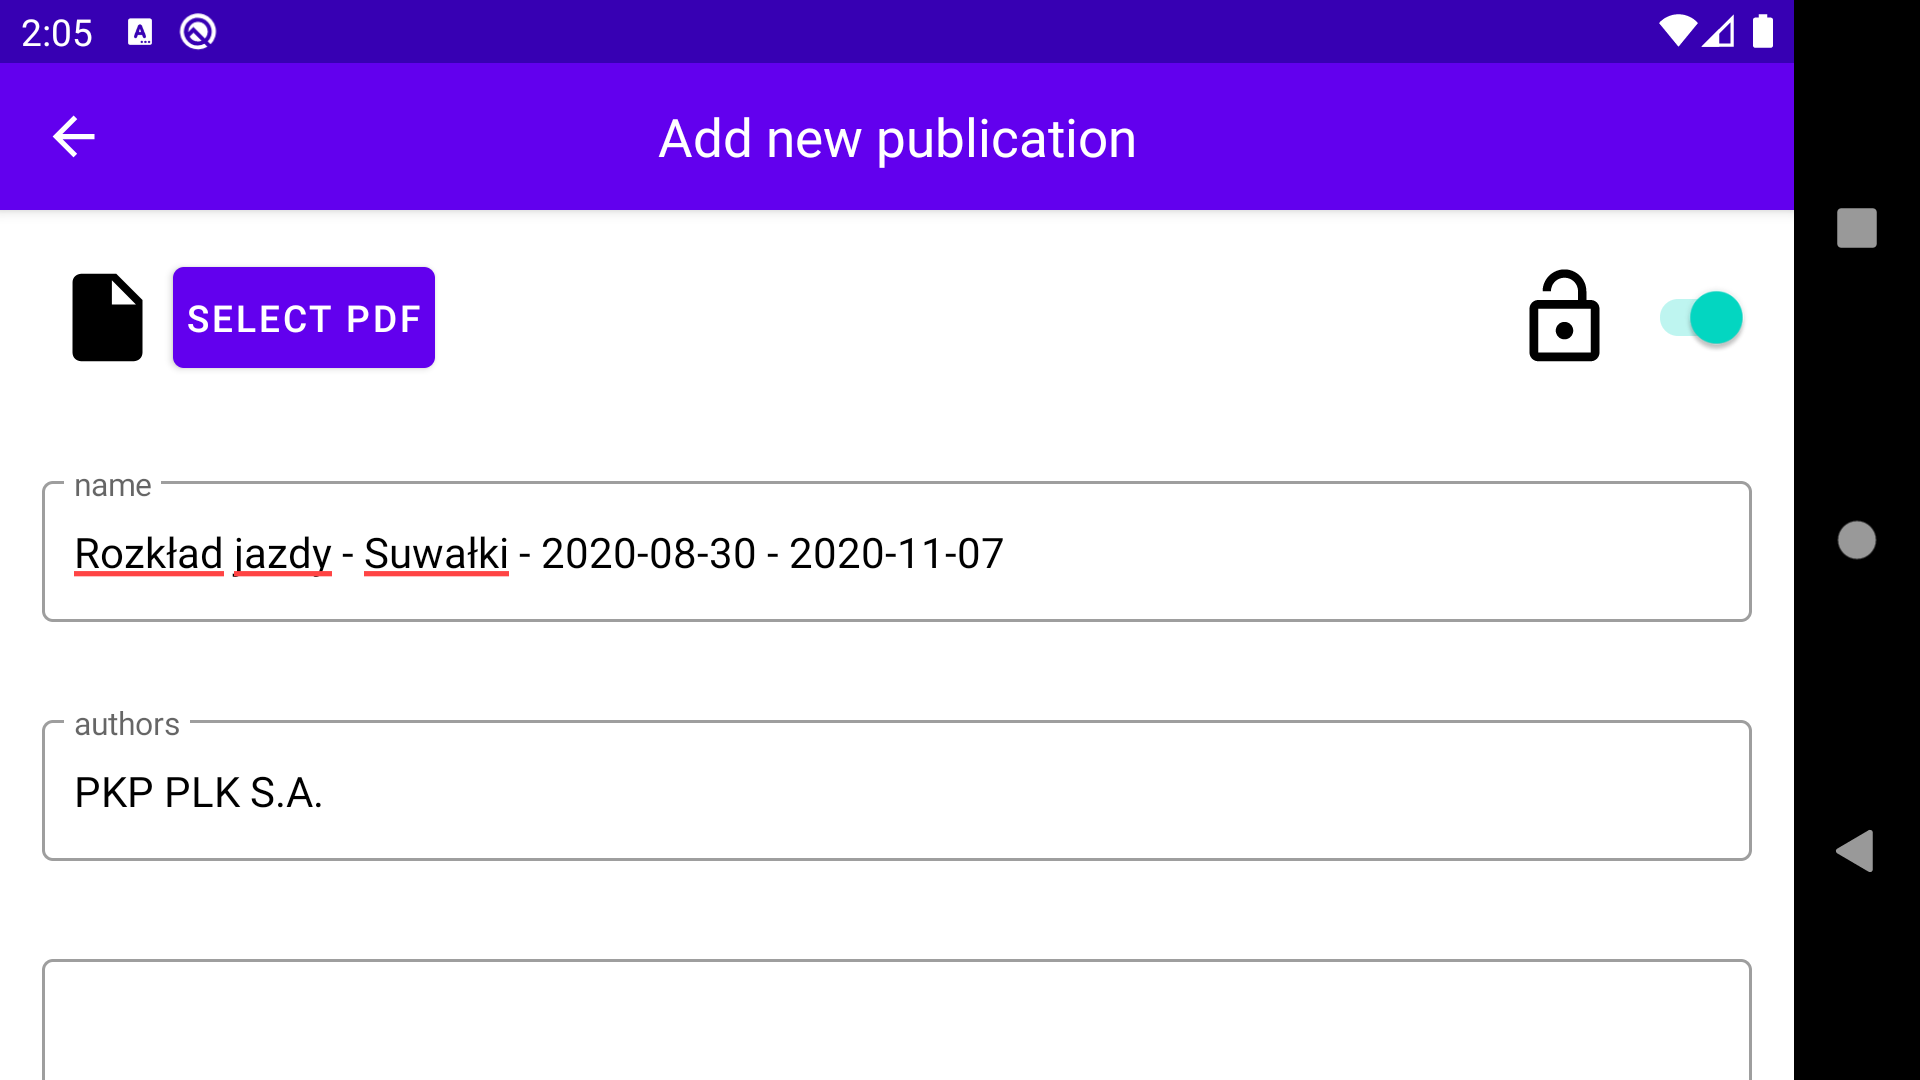
\includegraphics[scale=0.2]{\ImgPath/rys/screenshots/metadane.png}
	\end{center}
	\caption{Ekran szczegółów publikacji po przetworzeniu dokumentu zawierającego informacje w metadanych pliku.}
	\label{zrzutPrzetwarzanieMetadane}
\end{figure}

\subsection{Plik nie zawierający żadnych metadanych oraz numeru DOI}
W efekcie przetwarzania pliku, który nie posiada żadnych metadanych oraz numeru DOI nie uzyskano żadnych informacji dotyczących danej publikacji. W efekcie ekran szczegółów publikacji przedstawiony na Rysunku 6.10 nie zawiera żadnych informacji. Aby publikacja mogła zostać dodana do bazy danych, użytkownik musi wprowadzić te dane ręcznie.

\begin{figure}[!htbp]
	\begin{center}
		\centering
		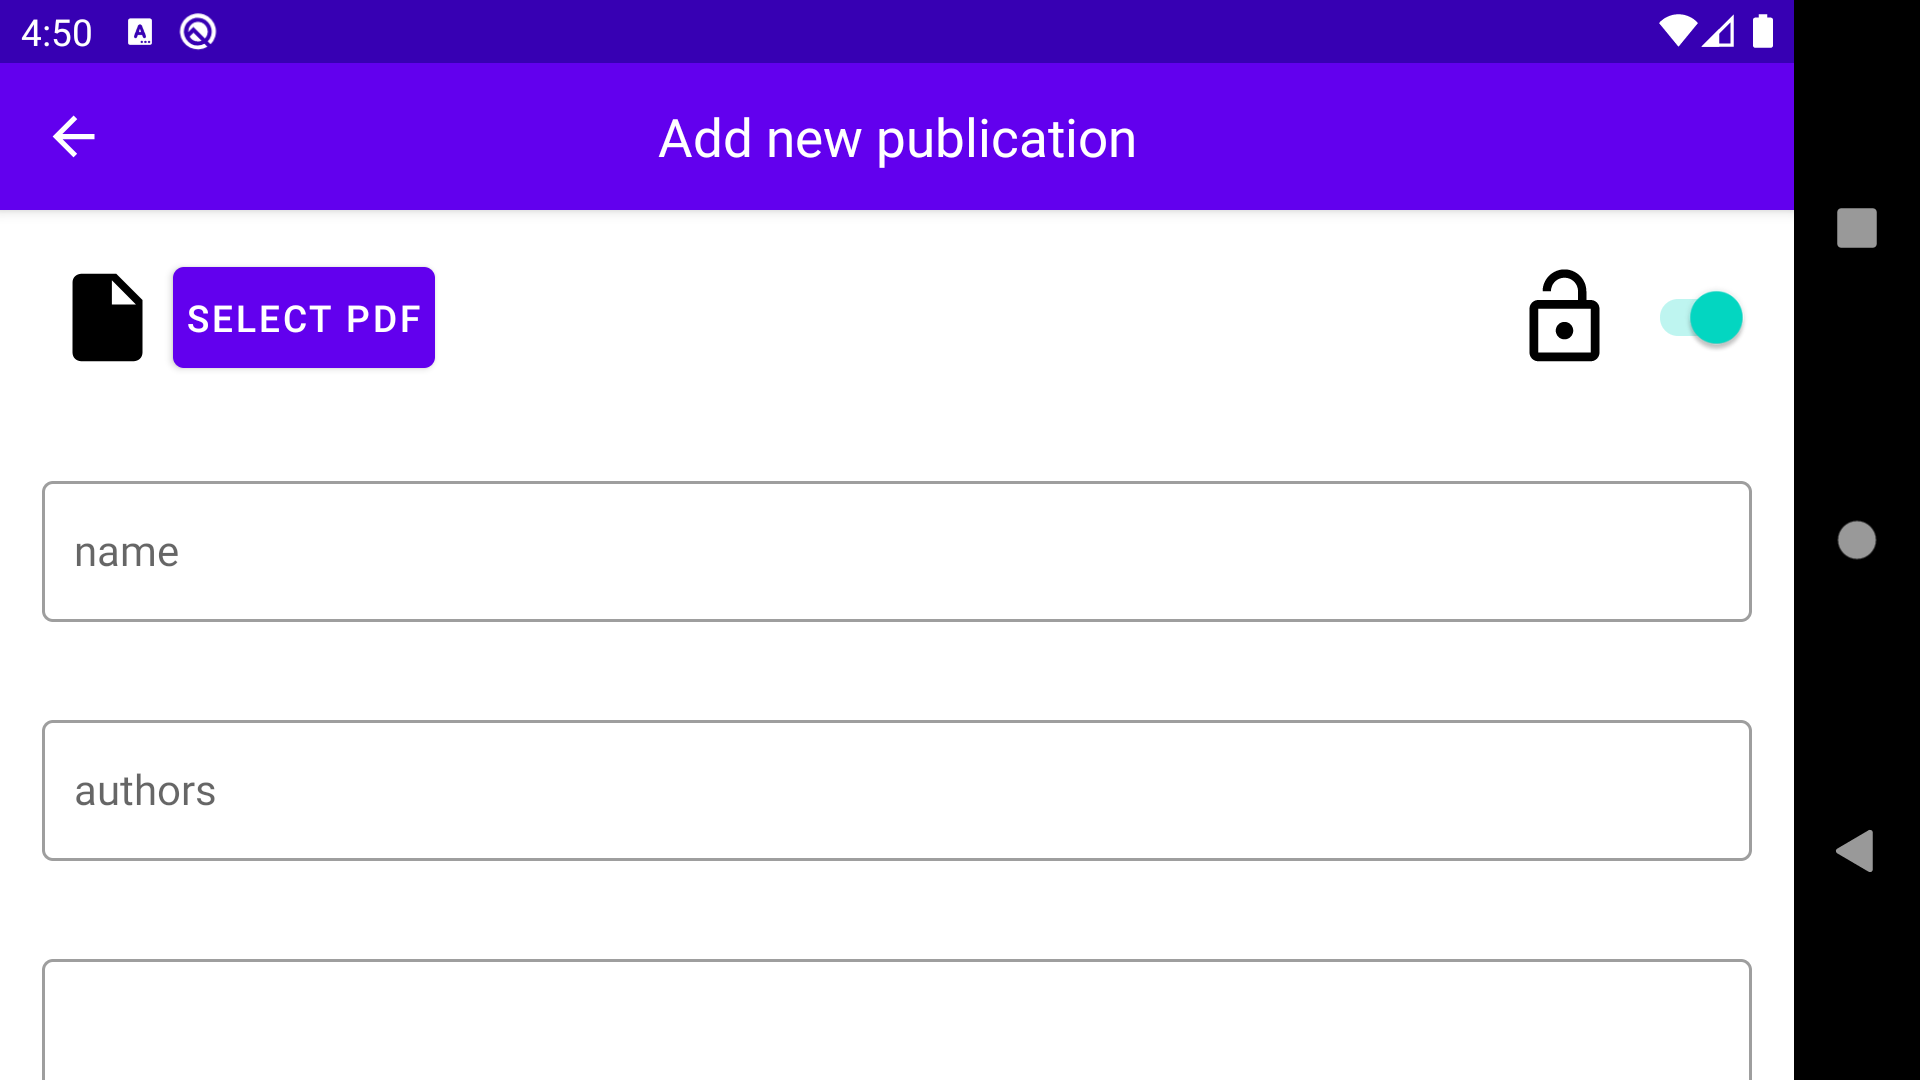
\includegraphics[scale=0.2]{\ImgPath/rys/screenshots/no_info_pdf.png}
	\end{center}
	\caption{Ekran szczegółów publikacji po przetworzeniu dokumentu nie zawierającego żadnych metadanych.}
	\label{zrzutPrzetwarzaniePusty}
\end{figure}




\section{Dodawanie, edycja i usuwanie publikacji.}

Ostatnia grupa testów będzie skupiać na podstawowych operacjach przeprowadzanych na przechowywanych publikacjach takich jak ich dodawanie, edycja oraz usuwanie. Sprawdzona zostanie także walidacja poprawności danych zapisywanych w ramach metadanych publikacji. Testy będą miały na celu przede wszystkim zweryfikować czy aplikacja kliencka poprawnie odczytuje i wysyła dane z aplikacji serwerowej, a także czy aplikacja serwerowa prawidłowo obsługuje żądania wysłane z aplikacji klienckiej.

\subsection{Dodawanie publikacji bez dodania pliku PDF}
Zgodnie z założeniami całego systemu, publikacja naukowa powinna być przechowywana w systemie jako plik PDF, dlatego też aplikacja nie powinna umożliwiać dodania publikacji, która nie posiada załączonego pliku PDF. Rysunek 6.11 przedstawia, że próba dodania publikacji bez pliku PDF zakończy się niepowodzeniem i wyświetleniem stosownego komunikatu.

\begin{figure}[!htbp]
	\begin{center}
		\centering
		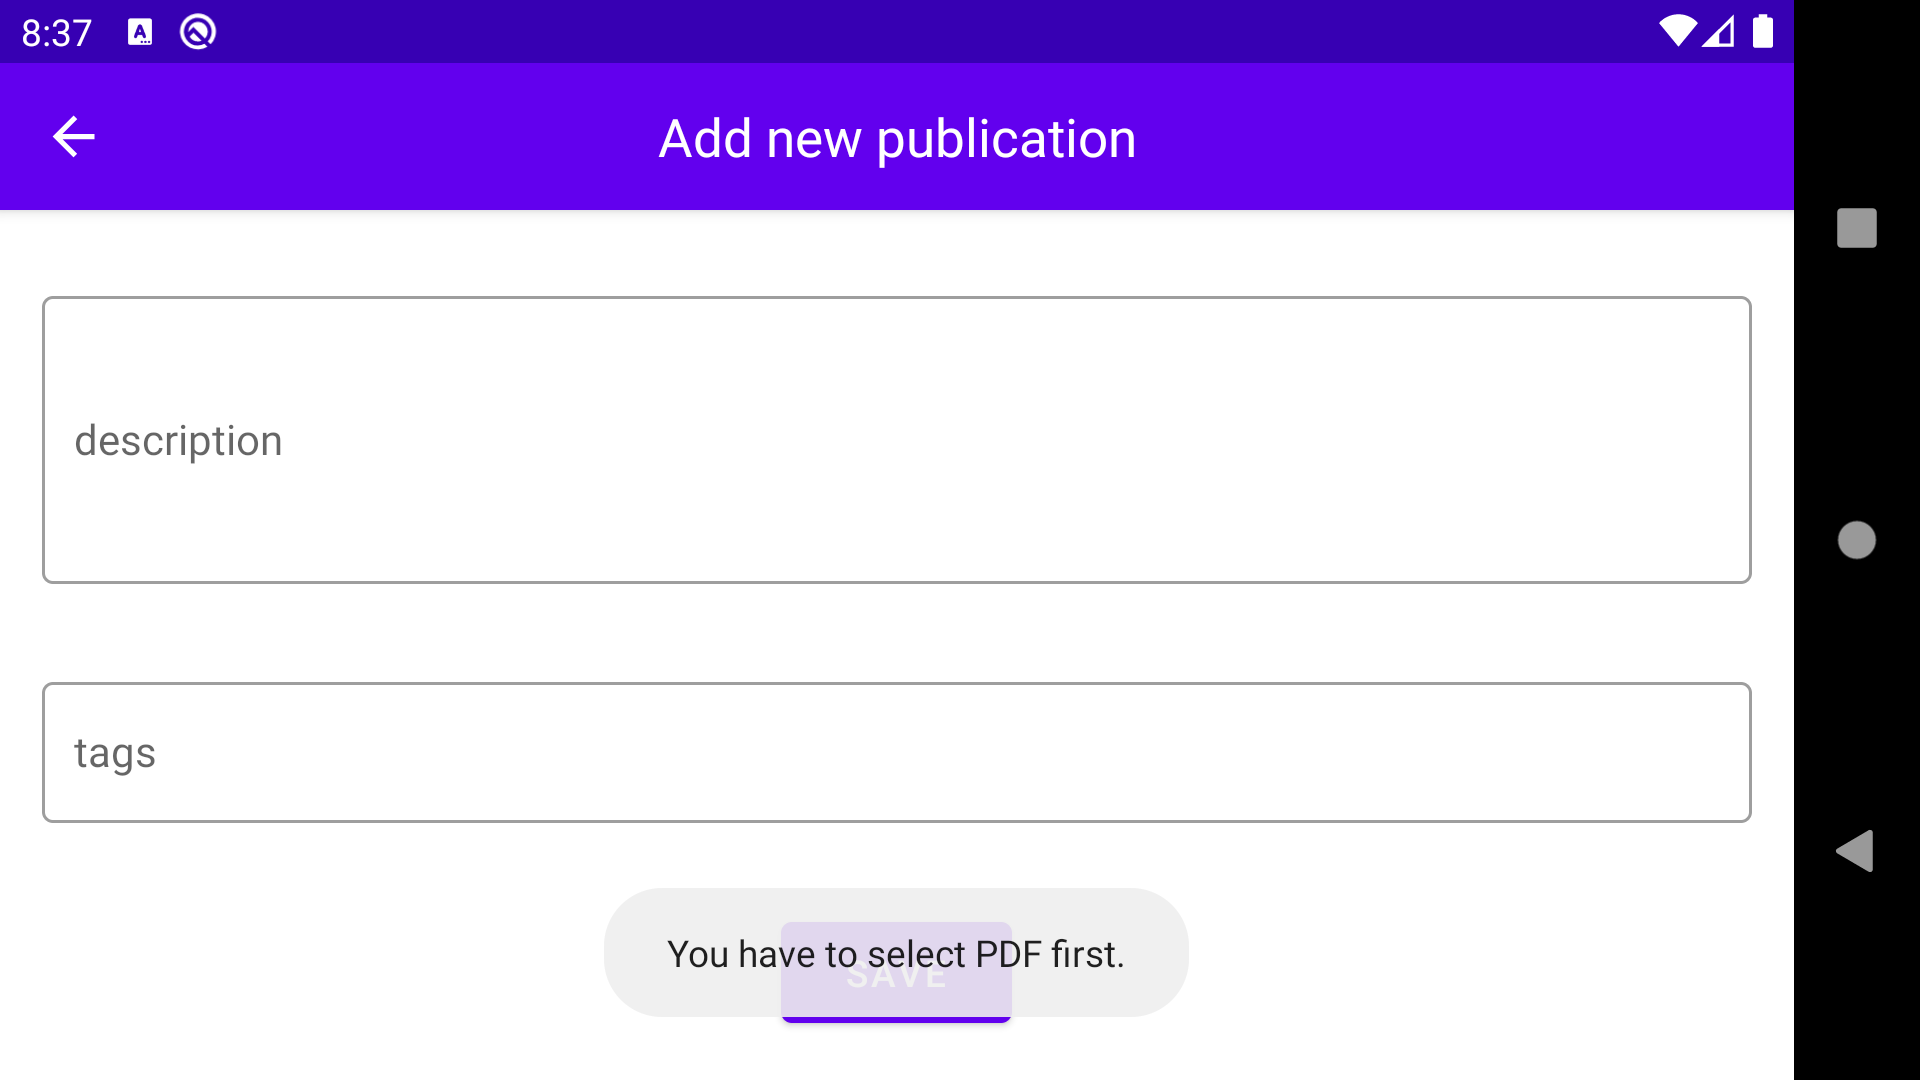
\includegraphics[scale=0.2]{\ImgPath/rys/screenshots/addEditDelete/no-pdf.png}
	\end{center}
	\caption{Ekran szczegółów publikacji z komunikatem o konieczności wyboru pliku PDF.}
	\label{zrzutPrzetwarzaniePusty}
\end{figure}

\subsection{Pełen proces dodawania publikacji}
Proces dodawania publikacji polega na wybraniu pliku PDF, a następnie na zredagowaniu odczytanych podczas przetwarzania pliku informacji dotyczących tytułu oraz autorów, a także na dodaniu opisu publikacji(przykład pokazany został na Rysunku 6.12). Następnie po przyciśnięciu przycisku \textit{Save} publikacja powinna zostać zapisana. Efekt tego procesu przedstawia Rysunek 6.13, co świadczy o poprawnym zakończeniu testu.

\pagebreak



\begin{figure}[!htbp]
	\begin{center}
		\centering
		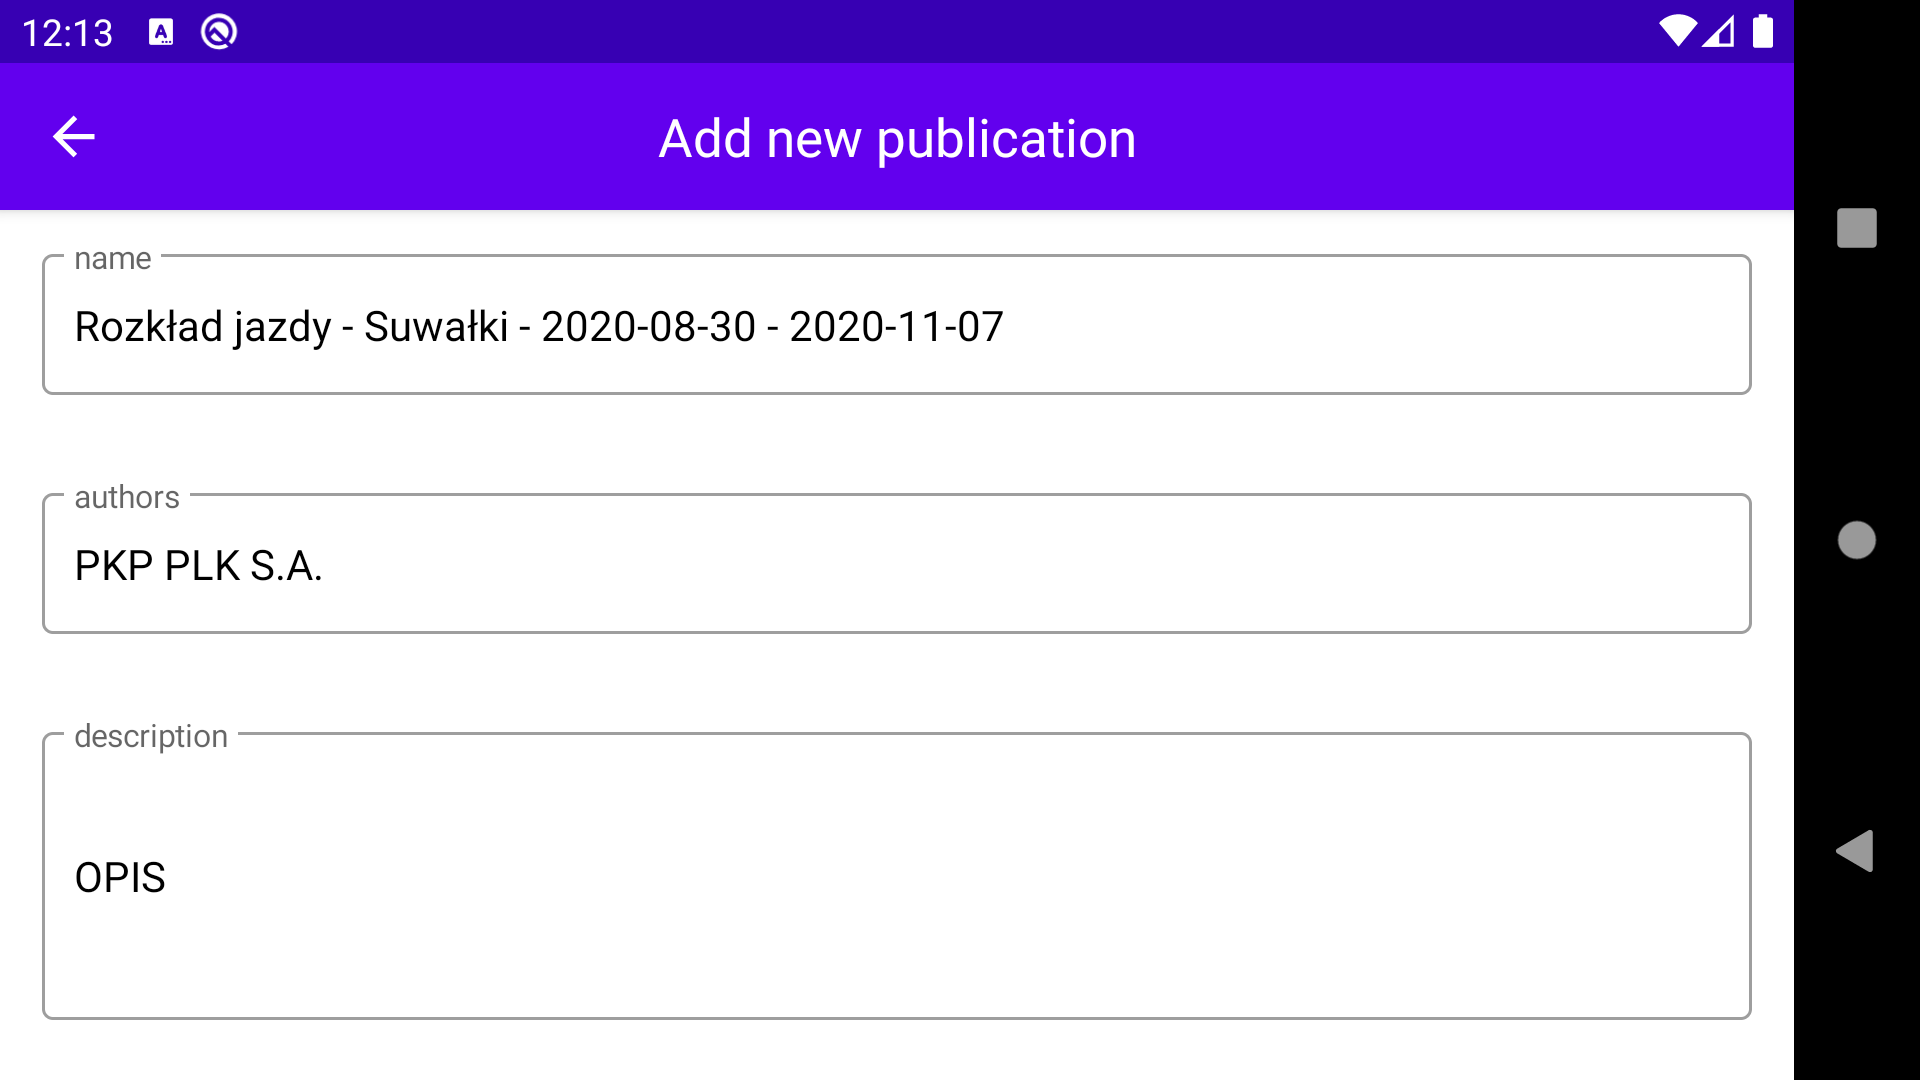
\includegraphics[scale=0.2]{\ImgPath/rys/screenshots/addEditDelete/add.png}
	\end{center}
	\caption{Ekran szczegółów publikacji przedstawiający uzupełnione pola nowej publikacji.}
	\label{zrzutSzczegolyPubPrzedDodaniem}
\end{figure}

\begin{figure}[!htbp]
	\begin{center}
		\centering
		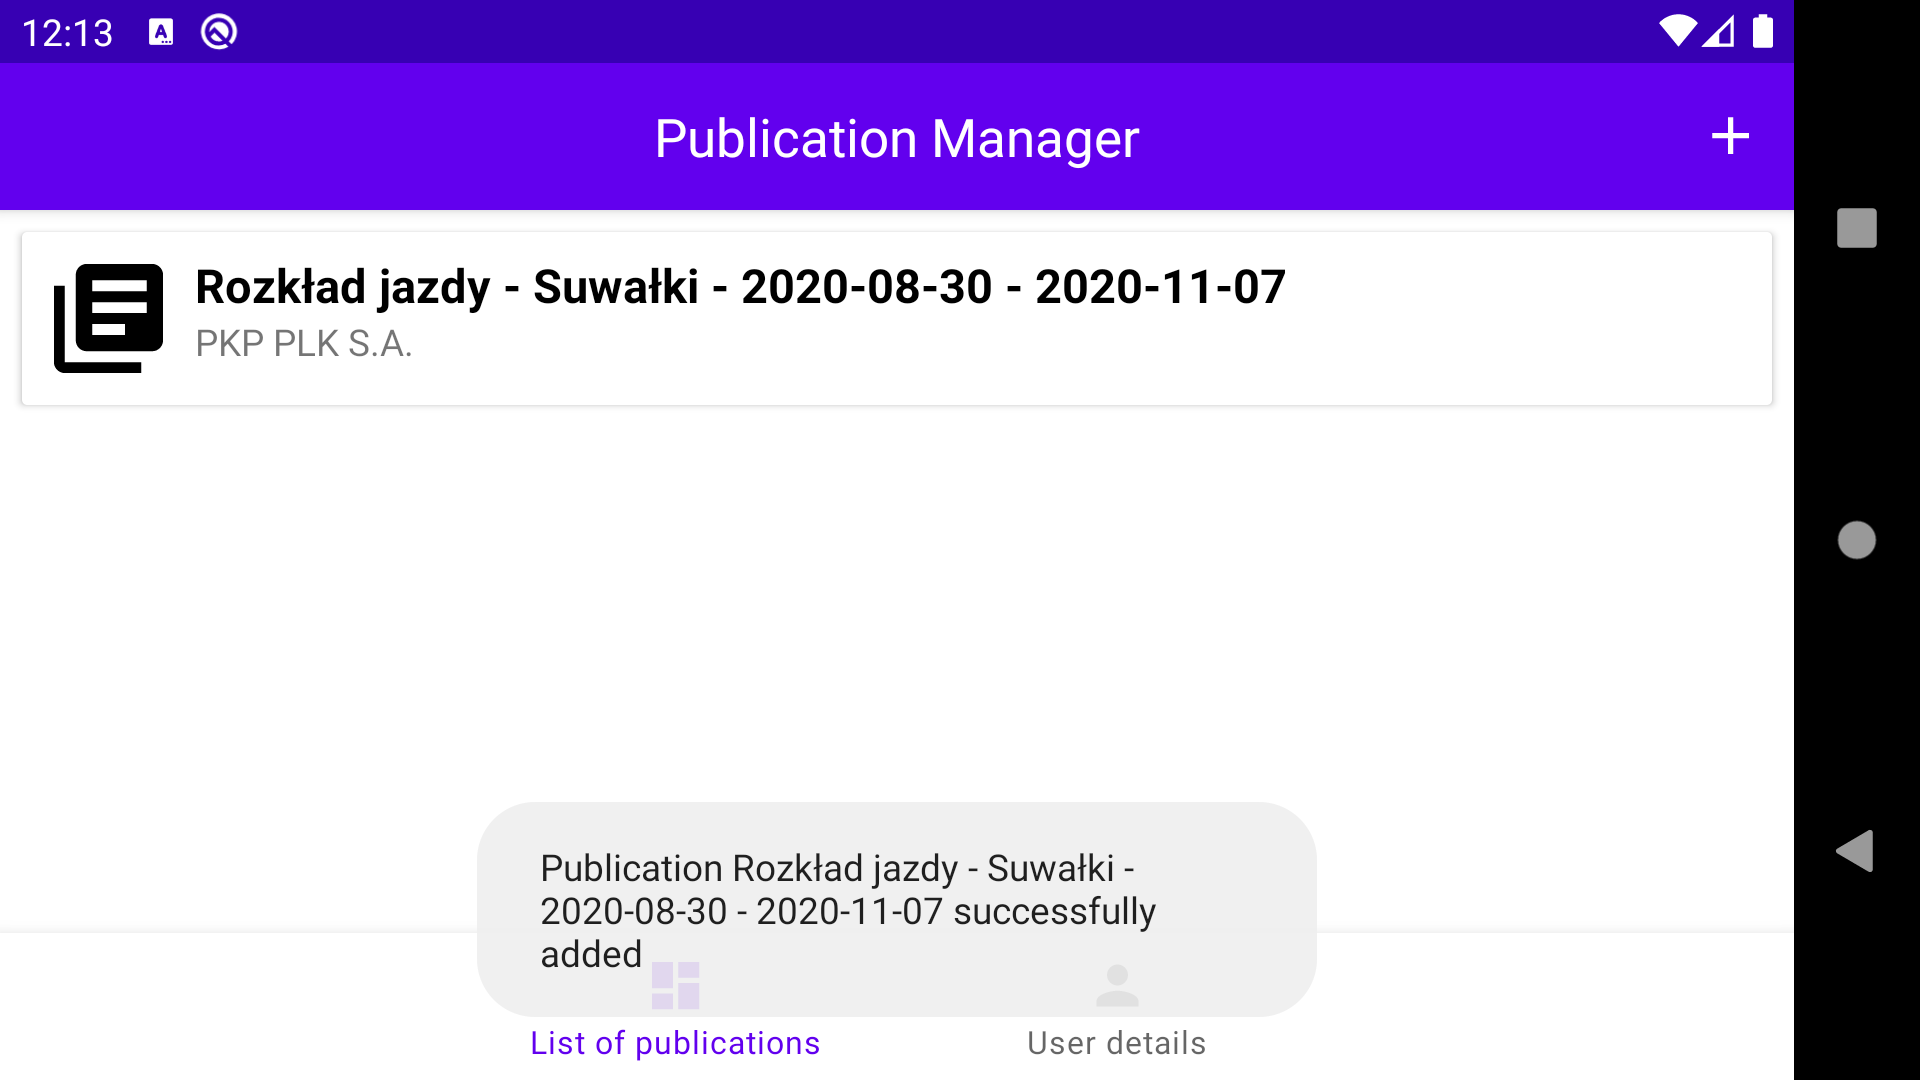
\includegraphics[scale=0.2]{\ImgPath/rys/screenshots/addEditDelete/after-add.png}
	\end{center}
	\caption{Ekran listy publikacji użytkownika prezentujący nowo dodaną publikację.}
	\label{zrzutListaPoDodaniu}
\end{figure}



\begin{figure}[!htbp]
	\begin{center}
		\centering
		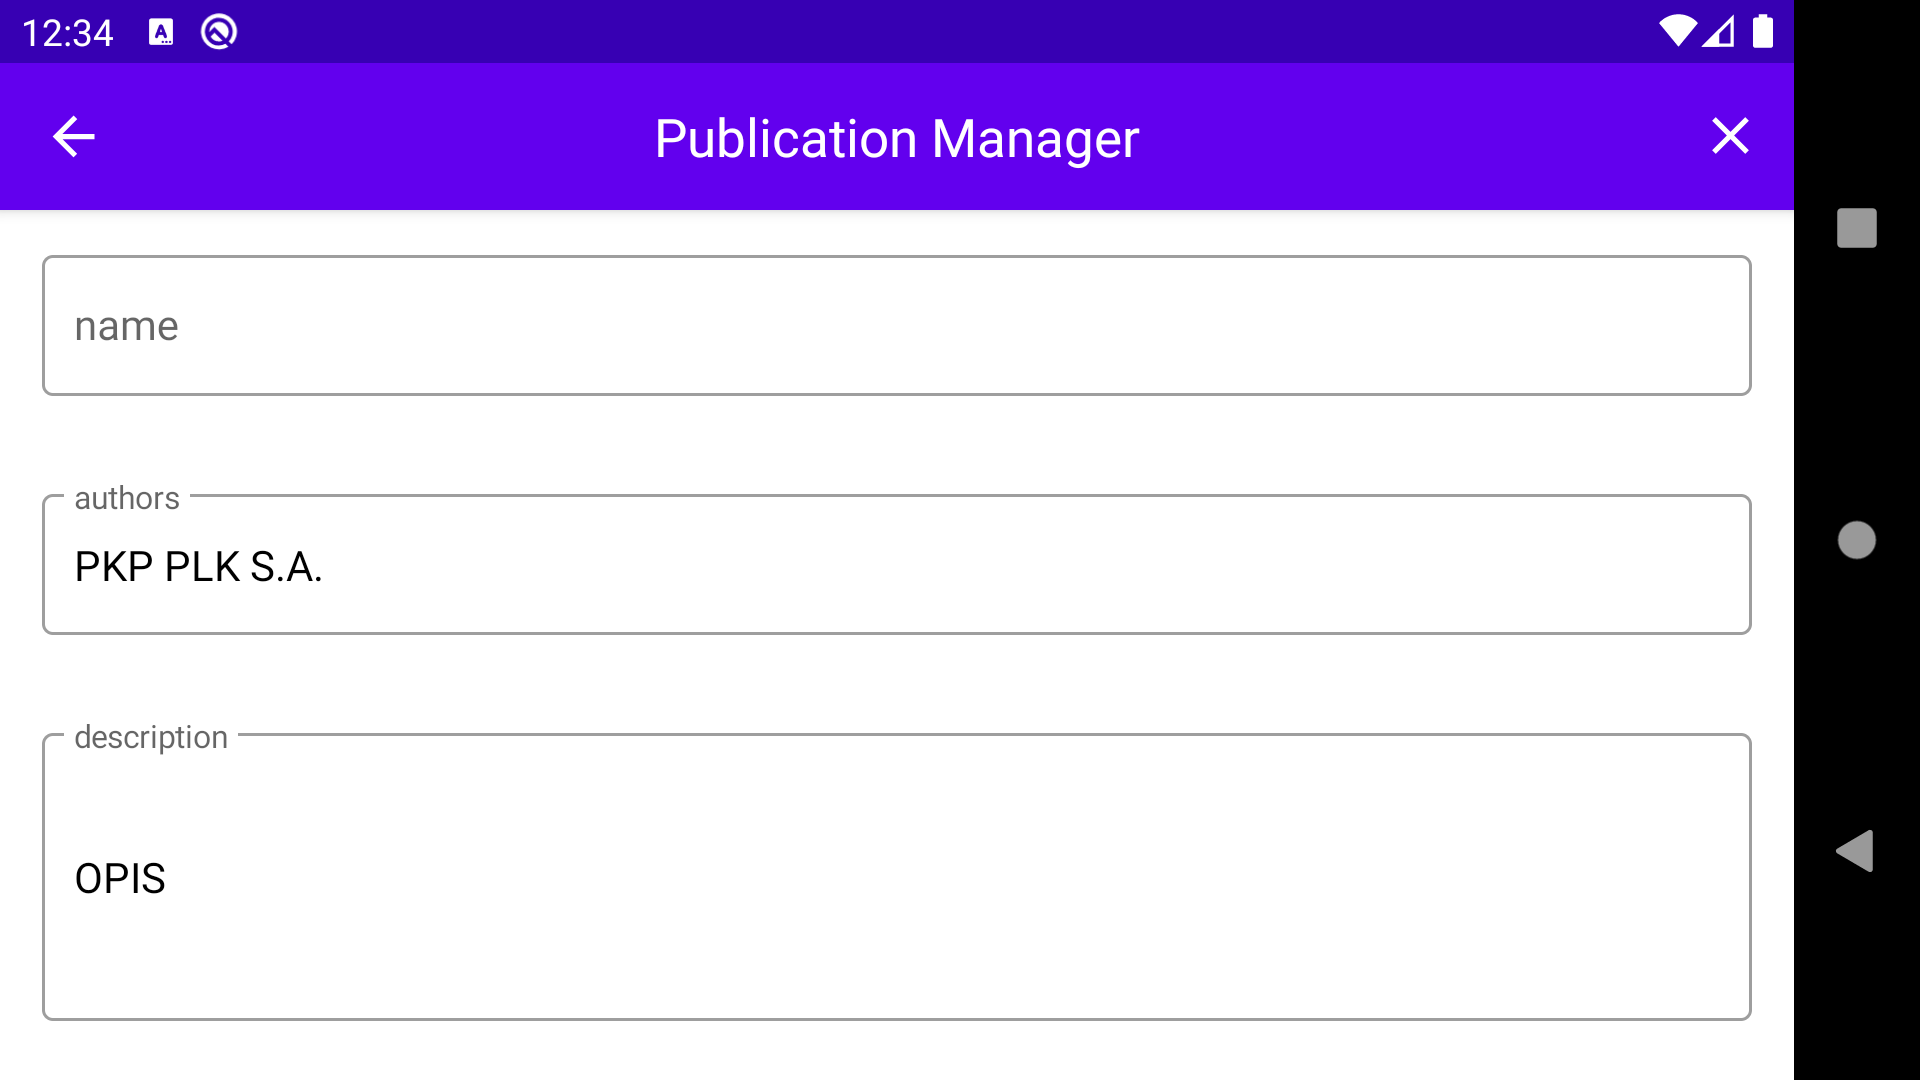
\includegraphics[scale=0.2]{\ImgPath/rys/screenshots/addEditDelete/edit-no-title.png}
	\end{center}
	\caption{Ekran szczegółów publikacji po przetworzeniu dokumentu nie zawierającego żadnych metadanych.}
	\label{zrzutPrzetwarzaniePusty}
\end{figure}

\begin{figure}[!htbp]
	\begin{center}
		\centering
		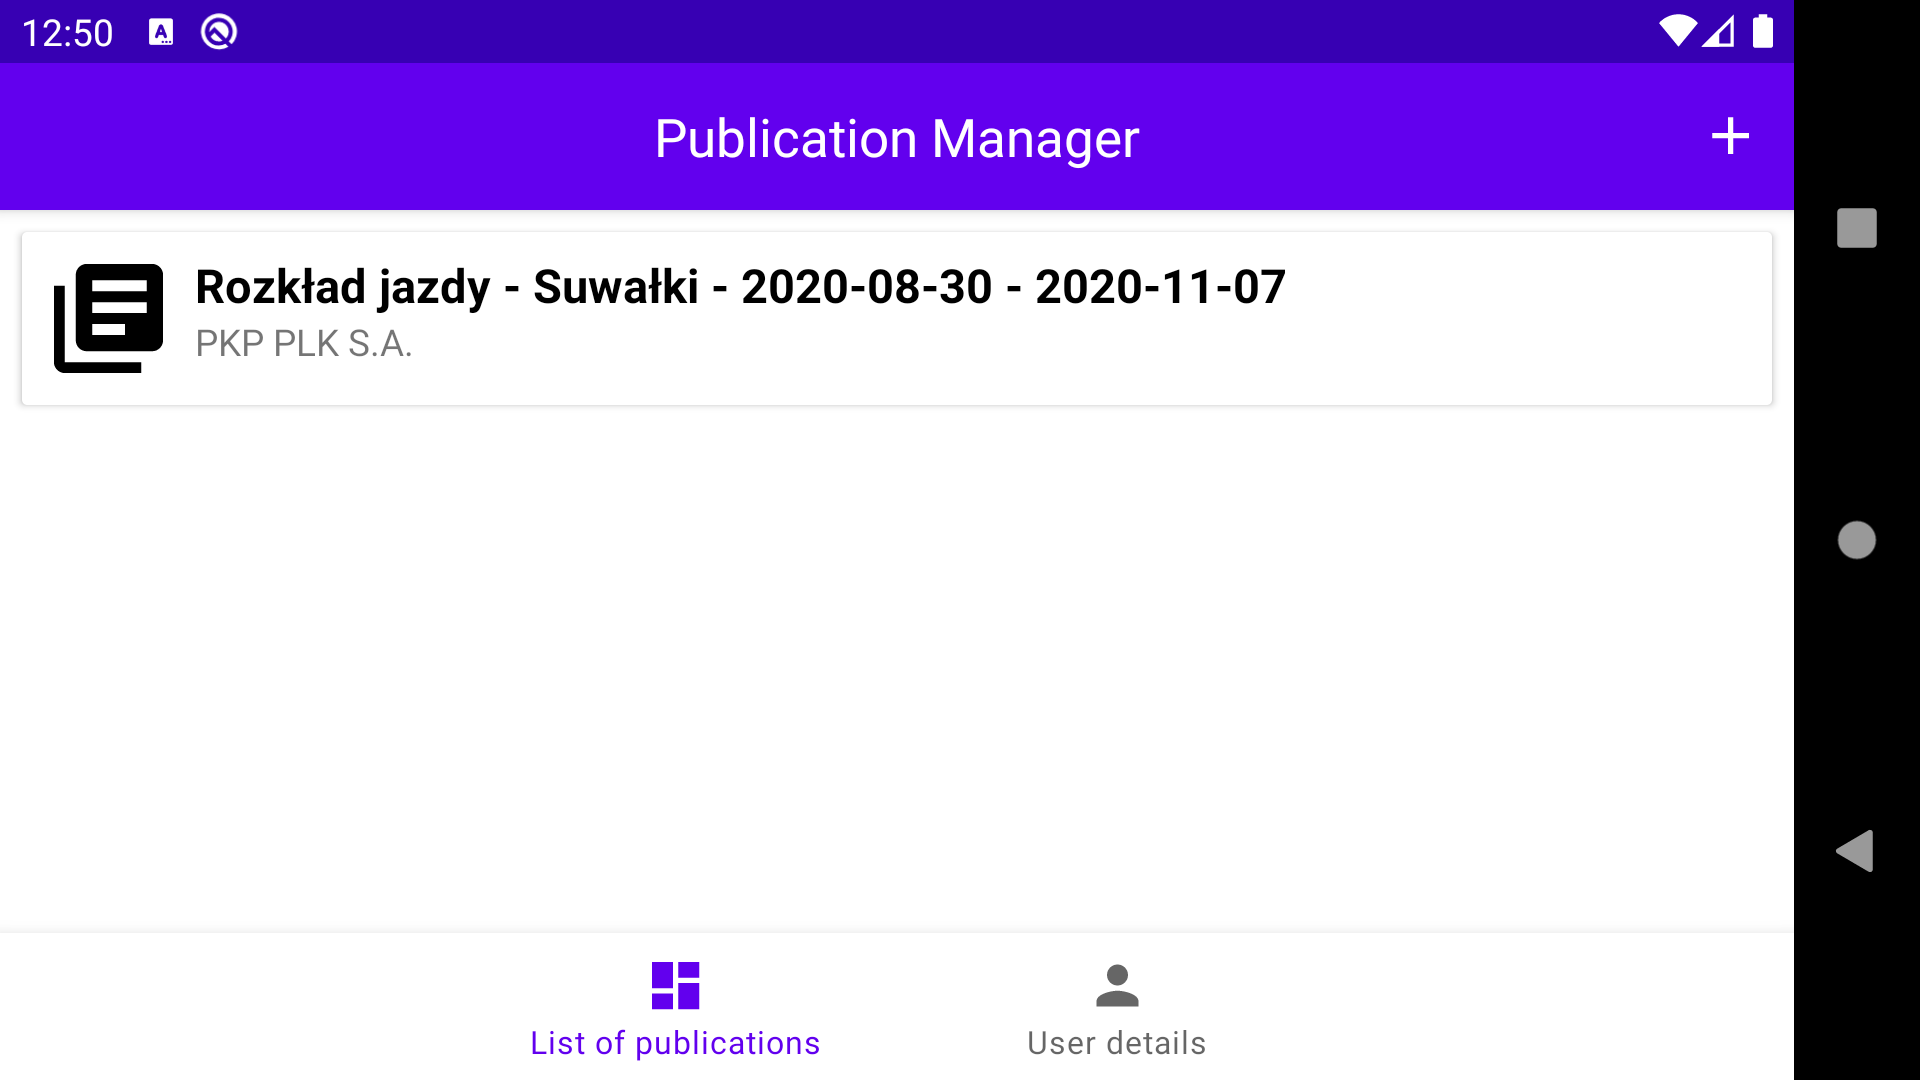
\includegraphics[scale=0.2]{\ImgPath/rys/screenshots/addEditDelete/after-edit-no-title.png}
	\end{center}
	\caption{Ekran listy publikacji użytkownika prezentujący zachowany tytuł publikacji.}
	\label{zrzutNieUsunietyTytul}
\end{figure}

\subsection{Edycja publikacji poprzez usunięcie tytułu}
Ze względu na to, że pole name jest obowiązkowe, w przypadku operacji usunięcia tytułu z publikacji, tytuł publikacji powinien zostać przywrócony do ostatniej postaci. Takie działanie zostało odnotowane i zaprezentowane na Rysunku 6.14, gdzie usunięty został tytuł publikacji \textit{,,Rozkład jazdy--Suwałki--2020--08--30-- 2020--11--07''}, a także na Rysunku 6.15 przedstawiającym  przywrócony tytuł edytowanej publikacji.

\subsection{Edycja publikacji poprzez zmianę danych}
W przypadku wprowadzania zmian w tytule, liście autorów lub w opisie publikacji, aplikacji powinna uaktualnić wartości, które zostały zmienione. Proces ten został przedstawiony gdzie na Rysunku 6.16 zapPrzetwarzaniePustyrezentowana została zedytowana publikacja, której stan pierwotny prezentuje Rysunek 6.12.

\begin{figure}[!htbp]
	\begin{center}
		\centering
		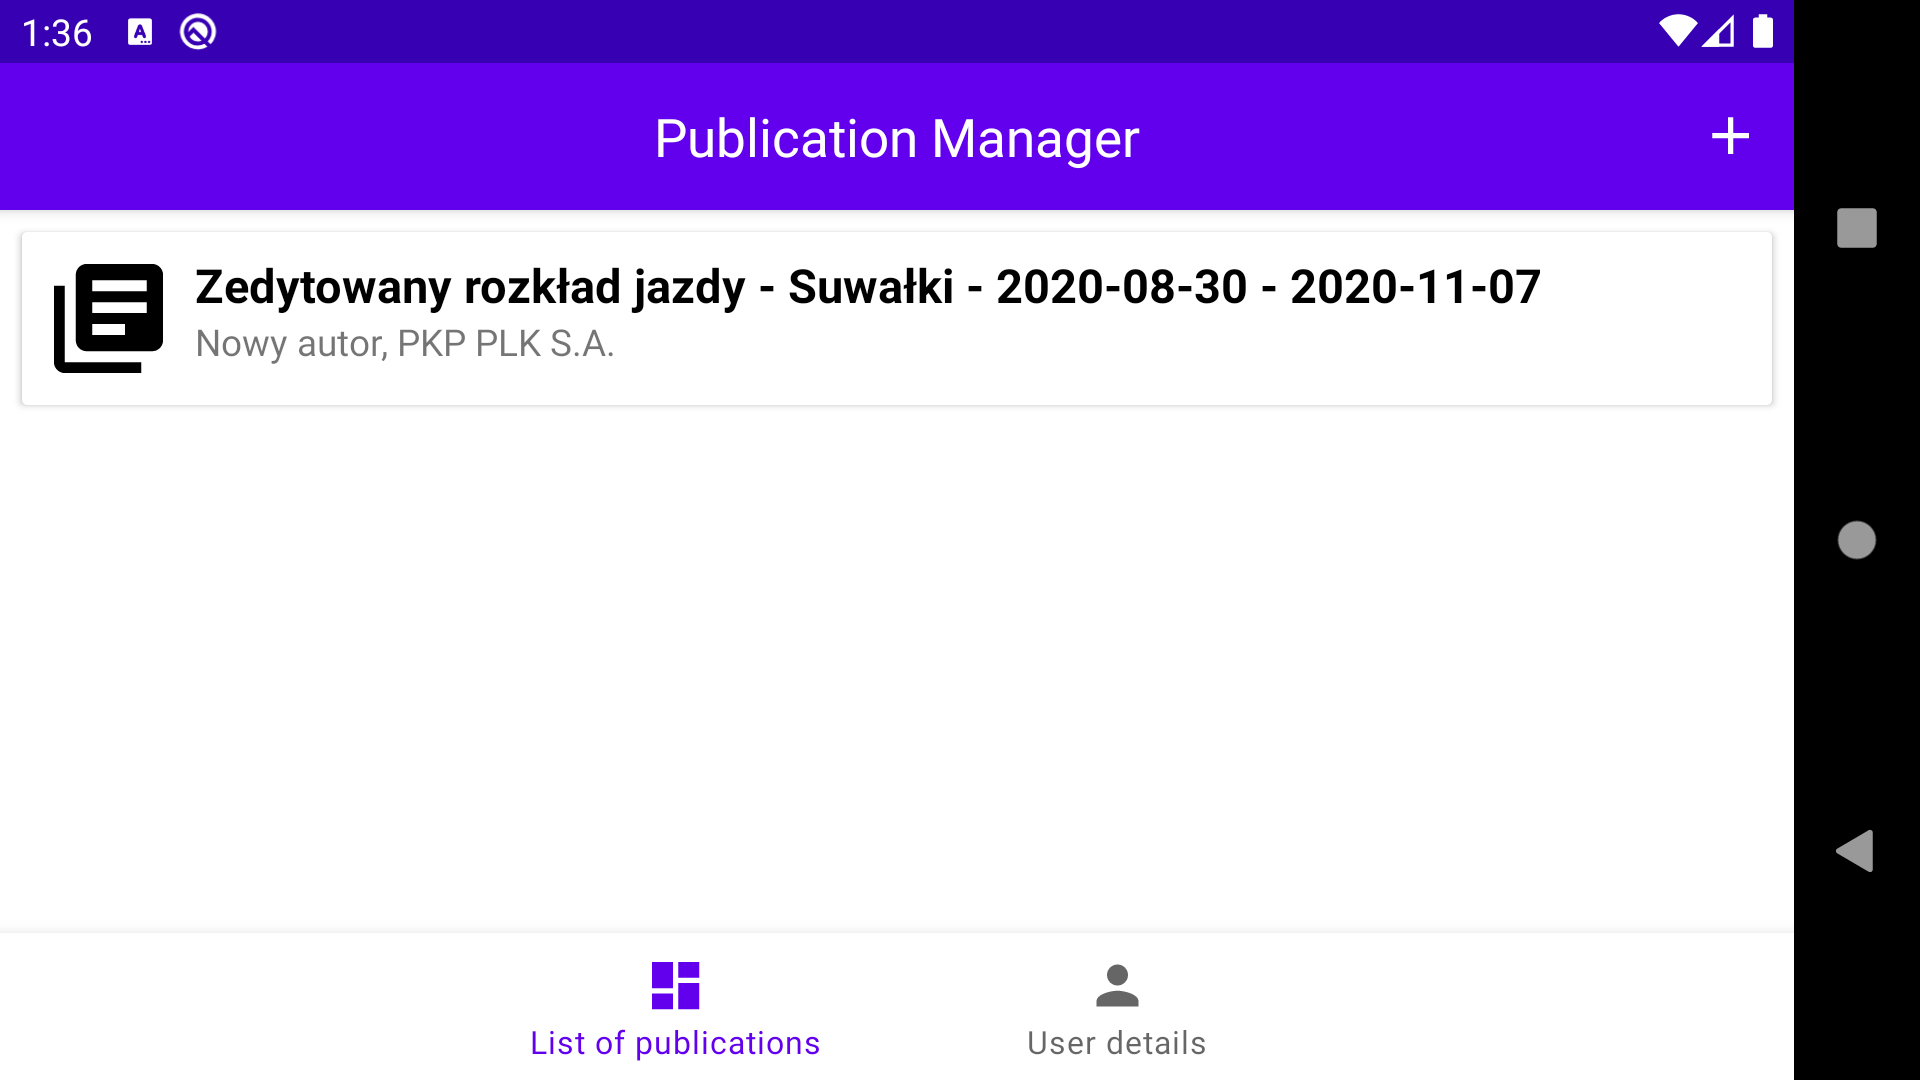
\includegraphics[scale=0.2]{\ImgPath/rys/screenshots/addEditDelete/after-edit.png}
	\end{center}
	\caption{Ekran szczegółów publikacji po przeprowadzeniu edycji publikacji.}
	\label{zrzutPoEdycji}
\end{figure}



\subsection{Usunięcie publikacji}
Proces usuwania publikacji wymaga wciśnięcia ikony z symbolem \textit{X}, która znajduje się w prawym górnym ekranu szczegółów aplikacji (Rysunek 6.17). Test usuwania zakończył się pomyślnie, co przedstawia pusta lista publikacji, a także stosowny komunikat przedstawiony na Rysunku 6.18

\begin{figure}[!htbp]
	\begin{center}
		\centering
		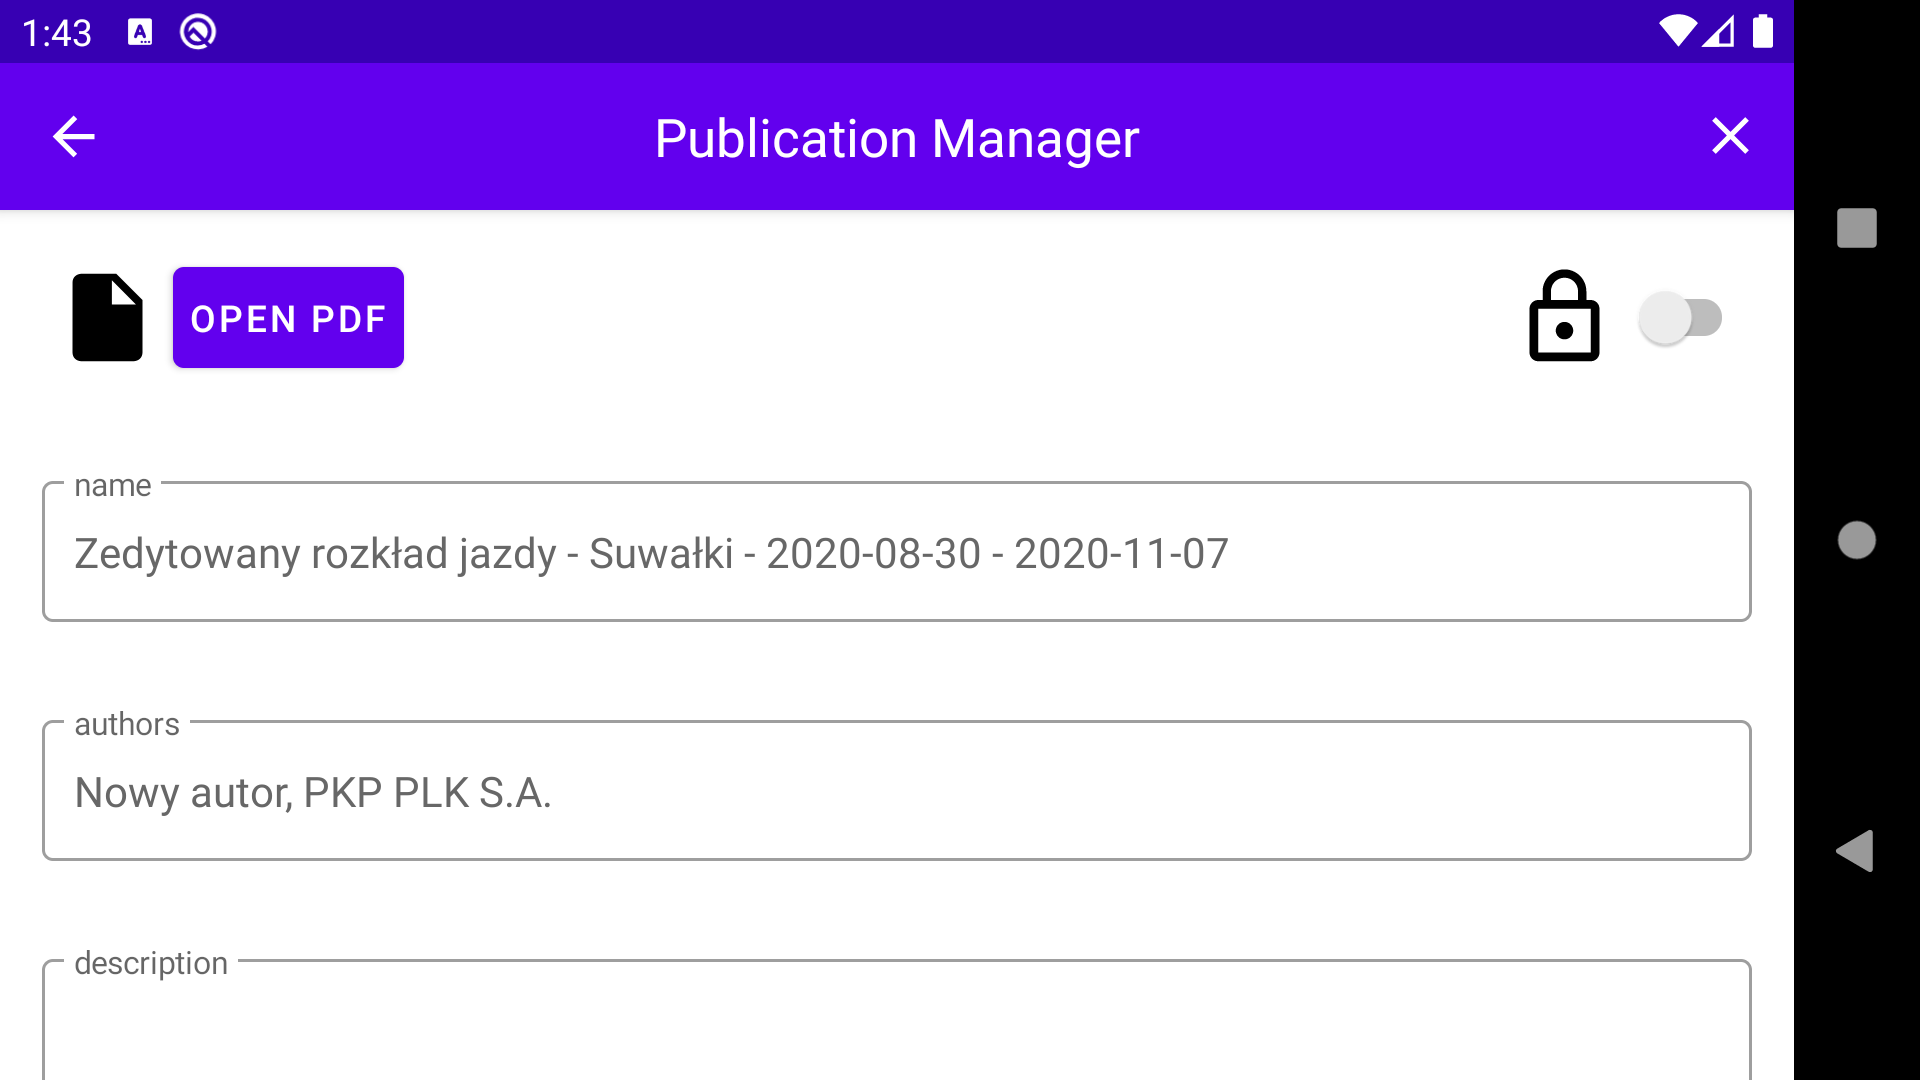
\includegraphics[scale=0.19]{\ImgPath/rys/screenshots/addEditDelete/before-delete.png}
	\end{center}
	\caption{Ekran szczegółów publikacji z przyciskiem do usuwania publikacji w prawym górnym rogu.}
	\label{zrzutUsuwaniePrzycisk}
\end{figure}

\begin{figure}[!htbp]
	\begin{center}
		\centering
		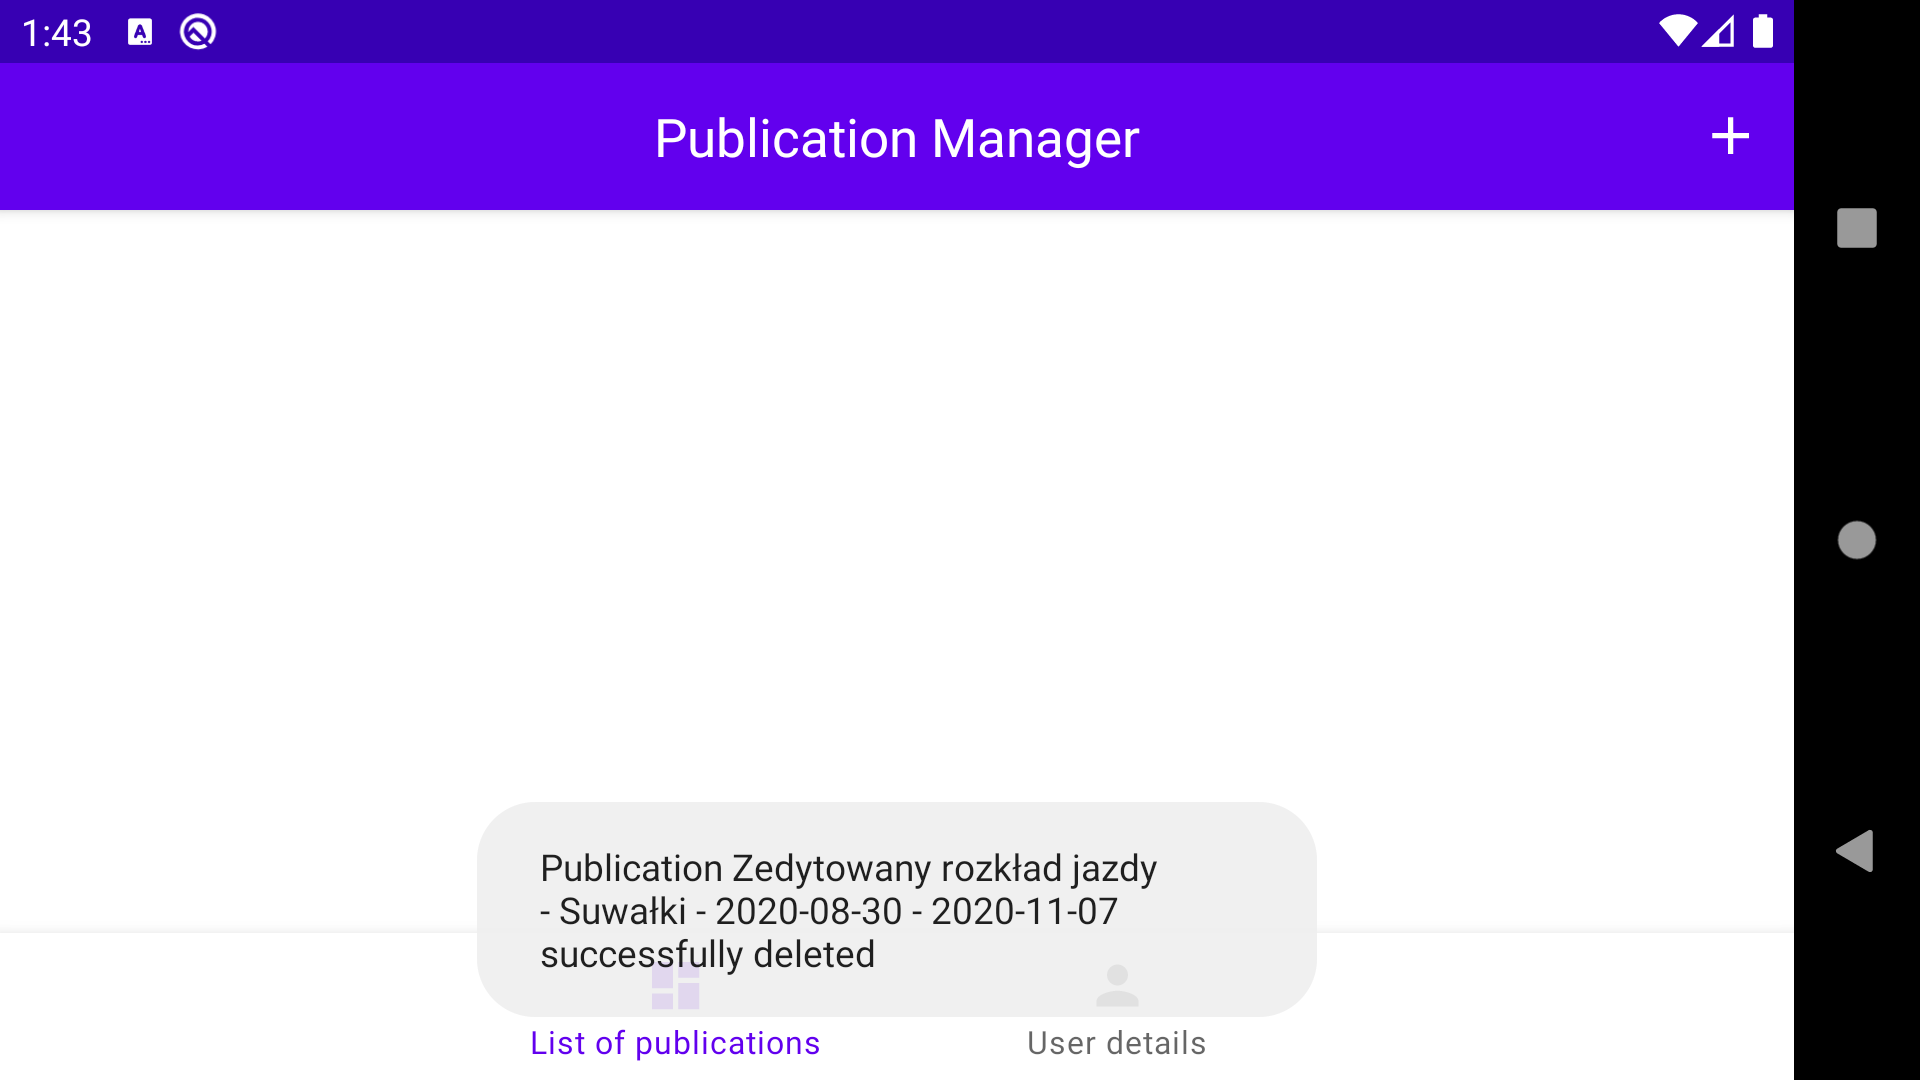
\includegraphics[scale=0.19]{\ImgPath/rys/screenshots/addEditDelete/after-delete.png}
	\end{center}
	\caption{Ekran z pustą listą publikacji użytkownika oraz komunikatem o pomyślnym usunięciu publikacji.}
	\label{zrzutUsuwanieLista}
\end{figure}



\chapter{Podsumowanie}
Celem projektu opisywanego w tej pracy było stworzenie systemu do zarządzania publikacjami naukowymi, którego główną funkcją będzie uzyskiwanie informacji dotyczących publikacji podczas procesu przetwarzania pliku. W tej pracy zaprezentowane zostały informacje dotyczące założeńm funkcji ale także szczegółów implementacyjnych aplikacji, która została wykonana. W pierwszym rozdziale tej pracy zostały zaprezentowane najważniejsze założenia całego systemu, które zostały w pełni spełnione:

\begin{enumerate}
	\item Aplikacja serwerowa została napisana przy użyciu Node.js oraz języka TypeScript;
	\item Baza danych wraz z aplikacją serwerową zostały skonteneryzowane w kontenery Dockera i są uruchamiane przy użyciu Docker--compose;
	\item Aplikacja kliencka uruchamiana jest na systemie Android i była testowana zarówno na urządzenia fizycznych, a także na emulatorze wbudowanym w środowisko Android Studio;
	\item Dla systemu został przygotowany autorski system rejestracji oraz logowania użytkowników;
	\item Podczas przetwarzania plików PDF, jeśli identyfikator DOI zostanie odnalezione, informacje dotyczące publikacji pobierane są z zewnętrznego API;
	\item Zarówno aplikacja serwerowa jaki i kliencka, zostały podzielone na moduły o jak największej niezależności, co pozwala na ich rozbudowę;
	\item W trakcie tworzenia aplikacji klienckiej, wykorzystywany był wzorzec Model--View--ViewModel(MVVM), który jest obecnie jedynym z najbardziej zalecanych w kontekście aplikacji mobilnych na system Android.
\end{enumerate}

\section{Wnioski}
W trakcie powstawania systemu udało się wykonać w pełni funkcjonalny system obsługi publikacji, pomimo jego kształt zmieniał się pod wpływem trudności napotykanych podczas implementacji. Bardzo ważnym etapem projektu, było dogłębne przeanalizowanie projektu oraz analiza i ocena funkcji, które powinny zostać zaimplementowane w systemie. Dzięki dogłębnemu przeanalizowaniu stuktury metadanych plików PDF, ale także ich treści udało się ustalić pewne wzorce, które pozwoliły odczytywanie istotnych informacji zawartych w plikach. Ważny był także dobry dobór technologii -- struktura publikacji przechowywanych w bazie danych ulegała wielokrotnym zmianom, co jednak nie okazało się być dużą przeszkodą w trakcie implementacji, dzięki zastosowaniu nierelacyjnej bazy danych, która pozwalała na łatwą modyfikację struktury przechowywanych dokumentów.

Niezwykle istotna i pomocna okazała się także bardzo dobra dokumentacja systemy Android, która w pełni wspierała wykorzystywany w projekcie język Kotlin. Ta obserwacja wskazała, że jednym z najistotniejszych kryteriów wyboru technologii, powinna być właśnie jakość dokumentacji. Równie ważna okazała się sama popularność systemy Android oraz platformy Node.js, ponieważ skutkuje to znacznie szerszym wsparciem społeczności internetowej w trakcie rozwiązywanie problemów implementacyjnych. 

Bardzo ważną rzeczą było także tworzenie komponentów w sposób by były od siebie jak najbardziej niezależne i jak najbardziej uniwersalne. Dzięki temu znacznie łatwiej udało wprowadzać się zmiany, ale także ograniczyć ilość kodu, jak miało to miejsce podczas tworzenia modułu autoryzacji użytkowników, dzięki wykorzystaniu interfejsu \textit{IOwnership}, który pozwolił na pisanie znacznie ogólniejszych i bardziej uniwersalnych funkcji nadzorujących dostęp użytkowników do zasobów aplikacji. 

\section{Plany na przyszłość}
W trakcie realizacji systemu, dzięki coraz lepszemu rozpoznaniu problemu, zaczęły pojawiać się nowe pomysły na funkcje, które mogłyby zostać udostępnione użytkownikom. Część z nich pomimo tego, że zostały częściowo zaimplementowane nie znalazły się w finalnej wersji systemu, ze względu na ograniczenia czasowe. Między innymi były to:
\begin{itemize}
	\item Wprowadzenie publikacji publicznych, które mogę być przeglądane przez wszystkich użytkowników systemu. Obecnie publikacje mogą być przeglądane jedynie przez właścicieli;
	\item Możliwość współdzielenia publikacji prywatnych z innymi użytkownikowi. Funkcja ta została w pełni przygotowana po stronie aplikacji serwerowej, lecz ze względu na ograniczenia czasowe, nie została obsłużona w aplikacji klienckiej;
	\item Komentowanie publikacji współdzielonych z innymi użytkownikami. Podobnie jak wyżej wymieniona funkcja została zaimplementowana jedynie po stronie aplikacji serwerowej;
	\item Obserwowanie innych użytkowników i otrzymywanie powiadomień na temat nowych publikacji dodanych przez obserwowanych użytkowników;
	\item Rozszerzenie przetwarzania plików PDF o próbę odczytu metadanych publikacji bezpośrednio z treści pliku PDF.
\end{itemize}


\begin{thebibliography}{99}
\addcontentsline{toc}{chapter}{Bibliografia}

\bibitem{Express}{Mozilla Developers, \textit{Wprowadzenie do Express/Node}, dostęp październik 2020 \url{https://developer.mozilla.org/pl/docs/Learn/Server-side/Express_Nodejs/Introduction}}

\bibitem{Middleware}{Expressjs Developers, \textit{Writing middleware for use in Express apps}, dostęp Listopad 2020 \url{https://expressjs.com/en/guide/writing-middleware.html}}

\bibitem{Crossref}{Crossref Developers, \textit{Retrieve-metadata}, dostęp Listopad 2020 \url{https://www.crossref.org/education/retrieve-metadata/}}

\bibitem{Regex}{Mozilla Developers, \textit{Regular expressions}, dostęp Listopad 2020 \url{https://developer.mozilla.org/en-US/docs/Web/JavaScript/Guide/Regular_Expressions}}


\bibitem{NOSQL}{Krzysztof Waszkiewicz, \textit{Bazy danych nosql -- czym są? Nierelacyjna baza danych – jak ją wykorzystać?}, dostęp Listopad 2020 \url{https://itwiz.pl/czym-jest-nosql-jak-wykorzystac-nierelacyjne-bazy-danych/}}

\bibitem{NOSQL}{TypeScript Developers, \textit{TypeScript for JavaScript Programmers?}, dostęp Październik 2020 \url{https://www.typescriptlang.org/docs/handbook/typescript-in-5-minutes.html}}



\bibitem{MongoDBQueryNested}{MongoDB Developers, \textit{Query on Embedded/Nested Documents}, dostęp Listopad 2020\newline \url{https://docs.mongodb.com/manual/tutorial/query-embedded-documents/}}

\bibitem{MoongooseSubDocs}{Moongoose Developers, \textit{Query on Embedded/Nested Documents}, dostęp Listopad 2020\newline \url{https://mongoosejs.com/docs/subdocs.html}}

\bibitem{RedisDocs}{Node.js Redis Developers, \textit{Redis for Node.js}, dostęp Listopad 2020\newline \url{https://www.npmjs.com/package/redis}}

\bibitem{DockerIntro}{Wojciech Paciorkowski, \textit{Docker dla programistów, co to jest?}, dostęp Styczeń 2021\newline \url{https://sii.pl/blog/docker-dla-programistow-co-to-jest/}}

\bibitem{DockerComposeDocs}{Docker Developers, \textit{Get started with Docker Compose}, dostęp Listopad 2020\newline \url{https://docs.docker.com/compose/gettingstarted/}}

\bibitem{Bcrypt}{Bcrypt for Node.js Developers, \textit{Bcrypt for Node.js}, dostęp Listopad 2020\newline \url{https://www.npmjs.com/package/bcrypt}}

\bibitem{TokenAuthJWT}{Macy Ngan, \textit{Modern Token Authentication in Node with Express}, dostęp Listopad 2020\newline \url{https://developer.okta.com/blog/2019/02/14/modern-token-authentication-in-node-with-express}}

\bibitem{KotlinForAndroid}{Kotlin Developers, \textit{Using Kotlin for Android Development}, dostęp Grudzień 2020\newline \url{https://kotlinlang.org/docs/reference/android-overview.html}}

\bibitem{MVVM}{Jerzy Piechowiak, \textit{MVVM — wprowadzenie do wzorca}, dostęp Styczeń 2021\newline \url{https://blog.helion.pl/mvvm-wprowadzenie-wzorca/}}

\bibitem{AndroidBasicsKotlin}{Android Developers, \textit{Android basics in kotlin}, dostęp Listopad 2020 \newline \url{https://developer.android.com/courses/android-basics-kotlin}}


\bibitem{ACTIVITY}{Android Developers, \textit{Activity}, dostęp Styczeń 2021\newline \url{https://developer.android.com/jetpack/guide}}


\bibitem{AndroidAppAcrchitecture}{Android Developers, \textit{Guide to app architecture}, dostęp Styczeń 2021\newline \url{https://developer.android.com/reference/android/app/Activity}}

\bibitem{INTENT}{Android Developers, \textit{Intent}, dostęp Grudzień 2020\newline \url{https://developer.android.com/reference/android/content/Intent}}

\bibitem{RecyclerMVVM}{Atif Mukhtiar, \textit{Recycler View With MVVM Livedata}, dostęp Grudzień 2020\newline \url{https://medium.com/@atifmukhtar/recycler-view-with-mvvm-livedata-a1fd062d2280}}

\bibitem{RecyclerView}{Florian Walther, \textit{Simple RecyclerView in Kotlin}, dostęp Grudzień 2020\newline \url{https://codinginflow.com/tutorials/android/simple-recyclerview-kotlin/part-1-layouts-model-class}}

\bibitem{RetrofitCallbacks}{Norman Peitek, \textit{Java Basics for Retrofit — Callbacks}, dostęp Grudzień 2020\newline \url{https://futurestud.io/tutorials/java-basics-for-retrofit-callbacks}}   


\bibitem{RetrofitUpload}{Marcus Pöhls, \textit{Retrofit 2 — How to Upload Files to Server}, dostęp Grudzień 2020\newline \url{https://futurestud.io/tutorials/retrofit-2-how-to-upload-files-to-server}}         
\bibitem{SharedPreferences}{Android Developers, \textit{Save key-value data}, dostęp Grudzień 2020\newline \url{https://developer.android.com/training/data-storage/shared-preferences}}  
 

\bibitem{ContentProvider}{Android Developers, \textit{Content provider basics}, dostęp Grudzień 2020\newline \url{https://developer.android.com/guide/topics/providers/content-provider-basics}}   

\bibitem{FilePicker}{Ivan Andrianto, \textit{Android File Picker Example}, dostęp Grudzień 2020\newline \url{https://www.woolha.com/tutorials/android-file-picker-example}}  


    


\end{thebibliography}

\zakonczenie  % wklejenie recenzji i opinii

\end{document}
%+++ END +++
